% Options for packages loaded elsewhere
\PassOptionsToPackage{unicode}{hyperref}
\PassOptionsToPackage{hyphens}{url}
\documentclass[
]{article}
\usepackage{xcolor}
\usepackage[margin=1in]{geometry}
\usepackage{amsmath,amssymb}
\setcounter{secnumdepth}{-\maxdimen} % remove section numbering
\usepackage{iftex}
\ifPDFTeX
  \usepackage[T1]{fontenc}
  \usepackage[utf8]{inputenc}
  \usepackage{textcomp} % provide euro and other symbols
\else % if luatex or xetex
  \usepackage{unicode-math} % this also loads fontspec
  \defaultfontfeatures{Scale=MatchLowercase}
  \defaultfontfeatures[\rmfamily]{Ligatures=TeX,Scale=1}
\fi
\usepackage{lmodern}
\ifPDFTeX\else
  % xetex/luatex font selection
\fi
% Use upquote if available, for straight quotes in verbatim environments
\IfFileExists{upquote.sty}{\usepackage{upquote}}{}
\IfFileExists{microtype.sty}{% use microtype if available
  \usepackage[]{microtype}
  \UseMicrotypeSet[protrusion]{basicmath} % disable protrusion for tt fonts
}{}
\makeatletter
\@ifundefined{KOMAClassName}{% if non-KOMA class
  \IfFileExists{parskip.sty}{%
    \usepackage{parskip}
  }{% else
    \setlength{\parindent}{0pt}
    \setlength{\parskip}{6pt plus 2pt minus 1pt}}
}{% if KOMA class
  \KOMAoptions{parskip=half}}
\makeatother
\usepackage{color}
\usepackage{fancyvrb}
\newcommand{\VerbBar}{|}
\newcommand{\VERB}{\Verb[commandchars=\\\{\}]}
\DefineVerbatimEnvironment{Highlighting}{Verbatim}{commandchars=\\\{\}}
% Add ',fontsize=\small' for more characters per line
\usepackage{framed}
\definecolor{shadecolor}{RGB}{248,248,248}
\newenvironment{Shaded}{\begin{snugshade}}{\end{snugshade}}
\newcommand{\AlertTok}[1]{\textcolor[rgb]{0.94,0.16,0.16}{#1}}
\newcommand{\AnnotationTok}[1]{\textcolor[rgb]{0.56,0.35,0.01}{\textbf{\textit{#1}}}}
\newcommand{\AttributeTok}[1]{\textcolor[rgb]{0.13,0.29,0.53}{#1}}
\newcommand{\BaseNTok}[1]{\textcolor[rgb]{0.00,0.00,0.81}{#1}}
\newcommand{\BuiltInTok}[1]{#1}
\newcommand{\CharTok}[1]{\textcolor[rgb]{0.31,0.60,0.02}{#1}}
\newcommand{\CommentTok}[1]{\textcolor[rgb]{0.56,0.35,0.01}{\textit{#1}}}
\newcommand{\CommentVarTok}[1]{\textcolor[rgb]{0.56,0.35,0.01}{\textbf{\textit{#1}}}}
\newcommand{\ConstantTok}[1]{\textcolor[rgb]{0.56,0.35,0.01}{#1}}
\newcommand{\ControlFlowTok}[1]{\textcolor[rgb]{0.13,0.29,0.53}{\textbf{#1}}}
\newcommand{\DataTypeTok}[1]{\textcolor[rgb]{0.13,0.29,0.53}{#1}}
\newcommand{\DecValTok}[1]{\textcolor[rgb]{0.00,0.00,0.81}{#1}}
\newcommand{\DocumentationTok}[1]{\textcolor[rgb]{0.56,0.35,0.01}{\textbf{\textit{#1}}}}
\newcommand{\ErrorTok}[1]{\textcolor[rgb]{0.64,0.00,0.00}{\textbf{#1}}}
\newcommand{\ExtensionTok}[1]{#1}
\newcommand{\FloatTok}[1]{\textcolor[rgb]{0.00,0.00,0.81}{#1}}
\newcommand{\FunctionTok}[1]{\textcolor[rgb]{0.13,0.29,0.53}{\textbf{#1}}}
\newcommand{\ImportTok}[1]{#1}
\newcommand{\InformationTok}[1]{\textcolor[rgb]{0.56,0.35,0.01}{\textbf{\textit{#1}}}}
\newcommand{\KeywordTok}[1]{\textcolor[rgb]{0.13,0.29,0.53}{\textbf{#1}}}
\newcommand{\NormalTok}[1]{#1}
\newcommand{\OperatorTok}[1]{\textcolor[rgb]{0.81,0.36,0.00}{\textbf{#1}}}
\newcommand{\OtherTok}[1]{\textcolor[rgb]{0.56,0.35,0.01}{#1}}
\newcommand{\PreprocessorTok}[1]{\textcolor[rgb]{0.56,0.35,0.01}{\textit{#1}}}
\newcommand{\RegionMarkerTok}[1]{#1}
\newcommand{\SpecialCharTok}[1]{\textcolor[rgb]{0.81,0.36,0.00}{\textbf{#1}}}
\newcommand{\SpecialStringTok}[1]{\textcolor[rgb]{0.31,0.60,0.02}{#1}}
\newcommand{\StringTok}[1]{\textcolor[rgb]{0.31,0.60,0.02}{#1}}
\newcommand{\VariableTok}[1]{\textcolor[rgb]{0.00,0.00,0.00}{#1}}
\newcommand{\VerbatimStringTok}[1]{\textcolor[rgb]{0.31,0.60,0.02}{#1}}
\newcommand{\WarningTok}[1]{\textcolor[rgb]{0.56,0.35,0.01}{\textbf{\textit{#1}}}}
\usepackage{longtable,booktabs,array}
\newcounter{none} % for unnumbered tables
\usepackage{calc} % for calculating minipage widths
% Correct order of tables after \paragraph or \subparagraph
\usepackage{etoolbox}
\makeatletter
\patchcmd\longtable{\par}{\if@noskipsec\mbox{}\fi\par}{}{}
\makeatother
% Allow footnotes in longtable head/foot
\IfFileExists{footnotehyper.sty}{\usepackage{footnotehyper}}{\usepackage{footnote}}
\makesavenoteenv{longtable}
\usepackage{graphicx}
\makeatletter
\newsavebox\pandoc@box
\newcommand*\pandocbounded[1]{% scales image to fit in text height/width
  \sbox\pandoc@box{#1}%
  \Gscale@div\@tempa{\textheight}{\dimexpr\ht\pandoc@box+\dp\pandoc@box\relax}%
  \Gscale@div\@tempb{\linewidth}{\wd\pandoc@box}%
  \ifdim\@tempb\p@<\@tempa\p@\let\@tempa\@tempb\fi% select the smaller of both
  \ifdim\@tempa\p@<\p@\scalebox{\@tempa}{\usebox\pandoc@box}%
  \else\usebox{\pandoc@box}%
  \fi%
}
% Set default figure placement to htbp
\def\fps@figure{htbp}
\makeatother
\setlength{\emergencystretch}{3em} % prevent overfull lines
\providecommand{\tightlist}{%
  \setlength{\itemsep}{0pt}\setlength{\parskip}{0pt}}
\usepackage{booktabs}
\usepackage{longtable}
\usepackage{array}
\usepackage{multirow}
\usepackage{wrapfig}
\usepackage{float}
\usepackage{colortbl}
\usepackage{pdflscape}
\usepackage{tabu}
\usepackage{threeparttable}
\usepackage{threeparttablex}
\usepackage[normalem]{ulem}
\usepackage{makecell}
\usepackage{xcolor}
\usepackage{bookmark}
\IfFileExists{xurl.sty}{\usepackage{xurl}}{} % add URL line breaks if available
\urlstyle{same}
\hypersetup{
  pdftitle={Predicting Student Success: A Multi-Model Machine Learning Approach},
  pdfauthor={Dongyuan Gao, Ramiro, Cyriel},
  hidelinks,
  pdfcreator={LaTeX via pandoc}}

\title{Predicting Student Success: A Multi-Model Machine Learning
Approach}
\usepackage{etoolbox}
\makeatletter
\providecommand{\subtitle}[1]{% add subtitle to \maketitle
  \apptocmd{\@title}{\par {\large #1 \par}}{}{}
}
\makeatother
\subtitle{Early Warning System for Student Dropout Risk}
\author{Dongyuan Gao, Ramiro, Cyriel}
\date{2025-12-16}

\begin{document}
\maketitle

\section{Summary}\label{summary}

\textbf{Our Storyline:} Higher education institutions face significant
challenges with \textbf{student drop-outs}. A fictional university has
engaged our education consulting firm to diagnose why students drop out.
The university wants to \textbf{understand and improve academic
performance}, and design \textbf{interventions} that reduce failed
academic lives. Understanding which students are \textbf{at risk of
dropping out}, and timely support that can change academic and life
trajectories.

\textbf{Our Data:} We have chosen a real case dataset from
\textbf{University of California, Irvine (UCI)}, to simulate the
fictional case. We found the dataset because the data repository website
appeared once in our Machine Learning 1 lecture.

\textbf{Our Approach:} We analyzed \textbf{4,424 students} from a
Portuguese higher education institution using \textbf{six} machine
learning models to predict student outcomes (\textbf{Dropout},
\textbf{Enrolled}, \textbf{Graduate}) and \textbf{understand the factors
that drive academic success}.

\subsection{Key Findings:}\label{key-findings}

\begin{itemize}
\tightlist
\item
  \textbf{First semester performance is the strongest predictor} of
  subsequent academic outcomes across all models
\item
  \textbf{Non-linear relationships exist} between age, course load, and
  success rates---captured by GAMs but missed by traditional linear
  models
\item
  \textbf{Economic and financial factors} (GDP, unemployment,
  scholarship status, tuition payment) show systematic effects on
  student success
\item
  \textbf{GAMs consistently outperform traditional GLMs} by 2-5
  percentage points, revealing curved relationships in the data
\item
  \textbf{Model accuracy ranges from 75-90\%} depending on the
  prediction task, with graduation prediction achieving the highest
  discrimination (\textbf{AUC ≈ 0.87})
\end{itemize}

\textbf{Business Impact:} These models enable institutions to
\textbf{identify at-risk students early}, \textbf{allocate resources
efficiently}, and implement \textbf{targeted interventions} that can
improve graduation rates by \textbf{10-15\%}.

\begin{center}\rule{0.5\linewidth}{0.5pt}\end{center}

\section{1. Introduction \& Data
Context}\label{introduction-data-context}

\subsection{1.1 Motivation}\label{motivation}

\textbf{Student dropout} is a critical issue in higher education with
consequences for:

\begin{itemize}
\tightlist
\item
  \textbf{Students:} Lost time, financial burden, and psychological
  impact
\item
  \textbf{Institutions:} Revenue loss, reduced graduation rates,
  reputational damage
\item
  \textbf{Society:} Lost human capital and economic potential
\end{itemize}

By predicting \textbf{dropout risk early}, institutions can intervene
with:

\begin{itemize}
\tightlist
\item
  Academic support programs
\item
  Financial aid counseling
\item
  Mental health services
\item
  Personalized study plans
\end{itemize}

\subsection{1.2 Data Source and Selection
Process}\label{data-source-and-selection-process}

\subsubsection{Choosing Our Dataset}\label{choosing-our-dataset}

\emph{Our goal} for this project is to deliver a \emph{solid report}
while using it as an opportunity to \emph{enhance our understanding} of
\emph{machine learning concepts} and practices. With this in mind, we
explored several \emph{potential datasets} for our final analysis.

We considered \emph{three main options}. First, the Social Media Fact
Sheet from PEW Research Center, which would have allowed us to analyze
social media usage patterns. Second, medical quality service data in
Switzerland from the Federal Office of Public Health (available through
opendata.swiss). Third, student data for predicting dropout and academic
success from the UC Irvine Machine Learning Repository.

After careful consideration, we chose the third option from the UC
Irvine repository. The \textbf{data structure and scope align well with
our goal} of getting familiarized with machine learning concepts and
practices while producing a solid report as our first attempt in the ML
world. While the other two datasets were interesting to explore, their
structure, diversity, and scope did not suit our \emph{learning
objectives} as well as the student success dataset. For the exploration
experience, we didn't read any papers related to the dataset online
while doing the project.

\subsubsection{Dataset Characteristics}\label{dataset-characteristics}

\textbf{Source:} UCI Machine Learning Repository - Predict Students'
Dropout and Academic Success\\
\textbf{Institution:} Portuguese higher education institution\\
\textbf{Time Period:} Multiple academic years\\
\textbf{Sample Size:} 4,424 students with 37 variables (e.g., age,
1st-semester grades, credits completed)

The dataset provides a comprehensive view of student characteristics and
outcomes, making it well-suited for applying multiple machine learning
models.

\textbf{Target Variable (3 factors):}

\begin{itemize}
\tightlist
\item
  \textbf{Dropout:} Students who left the program (1,421 students, 32\%)
\item
  \textbf{Enrolled:} Students currently continuing (794 students, 18\%),
  in some models counted as binary `not-dropout'.
\item
  \textbf{Graduate:} Students who completed successfully (2,209
  students, 50\%)
\end{itemize}

The distribution shows a balanced dataset with a slight majority of
graduates. It reflects the institution's overall success rate and
provides sufficient samples across all outcome categories for model
training.

\subsection{1.3 Feature Categories and detailed
variables}\label{feature-categories-and-detailed-variables}

Our dataset includes \textbf{36 predictors} in the following categories:
Demographic Information, Socioeconomic Factors, Academic Background,
Academic Performance, Financial Indicators, and Macroeconomic Context.
To make the business case and model results easier to follow, the table
below summarizes the most important variables used.

\begingroup\fontsize{10}{12}\selectfont

\begin{longtable}[t]{>{\raggedright\arraybackslash}p{12em}>{\raggedright\arraybackslash}p{18em}>{\raggedright\arraybackslash}p{10em}}
\caption{\label{tab:variable-overview-table}Key dataset variables (collapsed view)}\\
\toprule
Variable & Meaning & Type\\
\midrule
\textbf{Target} & Student outcome (Dropout / Enrolled / Graduate) & Categorical (3 classes)\\
\textbf{Admission.grade} & Admission exam/entry score used for program entry & Numeric\\
\textbf{Previous.qualification..grade.} & Grade from the previous qualification (prior education) & Numeric\\
\textbf{Age.at.enrollment} & Student age when enrolling in the program & Numeric\\
\textbf{Gender} & Student gender (coded numerically in the dataset) & Categorical (coded)\\
\addlinespace
\textbf{Scholarship.holder} & Whether the student holds a scholarship (0/1) & Binary (0/1)\\
\textbf{Debtor} & Whether the student is classified as a debtor (0/1) & Binary (0/1)\\
\textbf{Tuition.fees.up.to.date} & Whether tuition fees are paid up to date (0/1) & Binary (0/1)\\
\textbf{Curricular.units.1st.sem..enrolled.} & Number of courses the student enrolled in (1st semester) & Count\\
\textbf{Curricular.units.1st.sem..approved.} & Number of courses successfully passed (1st semester) & Count\\
\addlinespace
\textbf{Curricular.units.1st.sem..grade.} & Average grade in the 1st semester (0–20 scale) & Numeric\\
\bottomrule
\end{longtable}
\endgroup{}

\subsubsection{Why This Dataset Works for Our
Analysis}\label{why-this-dataset-works-for-our-analysis}

The dataset is suitable for applying all required machine learning
methods:

\textbf{For Linear Regression:} We have \textbf{continuous grade
variables (0-20 scale)}, allowing us to predict second semester
performance based on first semester results and student characteristics.

\textbf{For Binomial GLM:} The three-class target can be converted to
\textbf{Graduate vs Dropout}, enabling logistic regression with
\textbf{interpretable odds ratios}.

\textbf{For Poisson GLM:} \textbf{Count variables} are present (approved
courses, evaluations, failed courses), making it ideal for count-based
modeling.

\textbf{For GAM, Neural Networks, and SVM:} The mix of
\textbf{continuous and categorical predictors} plus a
\textbf{classification task} lets us explore \textbf{non-linear
relationships} and \textbf{complex interactions}.

The dataset contains \textbf{4,424 observations}---large \emph{enough}
for robust train-test splits and complex \emph{training}, yet
manageable. With \textbf{36 predictors} across demographic, academic,
financial, and socioeconomic domains, we have the complexity to deliver
\textbf{insights for our client}.

\begin{center}\rule{0.5\linewidth}{0.5pt}\end{center}

\section{2. Exploratory Data Analysis}\label{exploratory-data-analysis}

\subsection{2.1 Target Variable
Distribution}\label{target-variable-distribution}

\begin{Shaded}
\begin{Highlighting}[]
\CommentTok{\# Create a bar plot with percentages}
\NormalTok{target\_summary }\OtherTok{\textless{}{-}}\NormalTok{ df }\SpecialCharTok{\%\textgreater{}\%}
  \FunctionTok{group\_by}\NormalTok{(Target) }\SpecialCharTok{\%\textgreater{}\%}
  \FunctionTok{summarise}\NormalTok{(}\AttributeTok{count =} \FunctionTok{n}\NormalTok{()) }\SpecialCharTok{\%\textgreater{}\%}
  \FunctionTok{mutate}\NormalTok{(}\AttributeTok{percentage =}\NormalTok{ count }\SpecialCharTok{/} \FunctionTok{sum}\NormalTok{(count) }\SpecialCharTok{*} \DecValTok{100}\NormalTok{)}

\FunctionTok{ggplot}\NormalTok{(target\_summary, }\FunctionTok{aes}\NormalTok{(}\AttributeTok{x =}\NormalTok{ Target, }\AttributeTok{y =}\NormalTok{ count, }\AttributeTok{fill =}\NormalTok{ Target)) }\SpecialCharTok{+}
  \FunctionTok{geom\_bar}\NormalTok{(}\AttributeTok{stat =} \StringTok{"identity"}\NormalTok{, }\AttributeTok{alpha =} \FloatTok{0.8}\NormalTok{) }\SpecialCharTok{+}
  \FunctionTok{geom\_text}\NormalTok{(}\FunctionTok{aes}\NormalTok{(}\AttributeTok{label =} \FunctionTok{paste0}\NormalTok{(}\FunctionTok{round}\NormalTok{(percentage, }\DecValTok{1}\NormalTok{), }\StringTok{"\%}\SpecialCharTok{\textbackslash{}n}\StringTok{(n="}\NormalTok{, count, }\StringTok{")"}\NormalTok{)),}
            \AttributeTok{vjust =} \SpecialCharTok{{-}}\FloatTok{0.5}\NormalTok{, }\AttributeTok{size =} \DecValTok{4}\NormalTok{) }\SpecialCharTok{+}
  \FunctionTok{scale\_fill\_manual}\NormalTok{(}\AttributeTok{values =} \FunctionTok{c}\NormalTok{(}\StringTok{"Dropout"} \OtherTok{=} \StringTok{"\#E74C3C"}\NormalTok{,}
                                \StringTok{"Enrolled"} \OtherTok{=} \StringTok{"\#F39C12"}\NormalTok{,}
                                \StringTok{"Graduate"} \OtherTok{=} \StringTok{"\#27AE60"}\NormalTok{)) }\SpecialCharTok{+}
  \FunctionTok{scale\_y\_continuous}\NormalTok{(}\AttributeTok{expand =} \FunctionTok{expansion}\NormalTok{(}\AttributeTok{mult =} \FunctionTok{c}\NormalTok{(}\DecValTok{0}\NormalTok{, }\FloatTok{0.1}\NormalTok{))) }\SpecialCharTok{+}
  \FunctionTok{labs}\NormalTok{(}\AttributeTok{title =} \StringTok{"Distribution of Student Outcomes"}\NormalTok{,}
       \AttributeTok{x =} \StringTok{"Outcome"}\NormalTok{, }\AttributeTok{y =} \StringTok{"Number of Students"}\NormalTok{, }\AttributeTok{fill =} \StringTok{"Outcome"}\NormalTok{) }\SpecialCharTok{+}
  \FunctionTok{theme}\NormalTok{(}\AttributeTok{legend.position =} \StringTok{"none"}\NormalTok{,}
        \AttributeTok{plot.title =} \FunctionTok{element\_text}\NormalTok{(}\AttributeTok{hjust =} \FloatTok{0.5}\NormalTok{, }\AttributeTok{face =} \StringTok{"bold"}\NormalTok{))}
\end{Highlighting}
\end{Shaded}

\begin{center}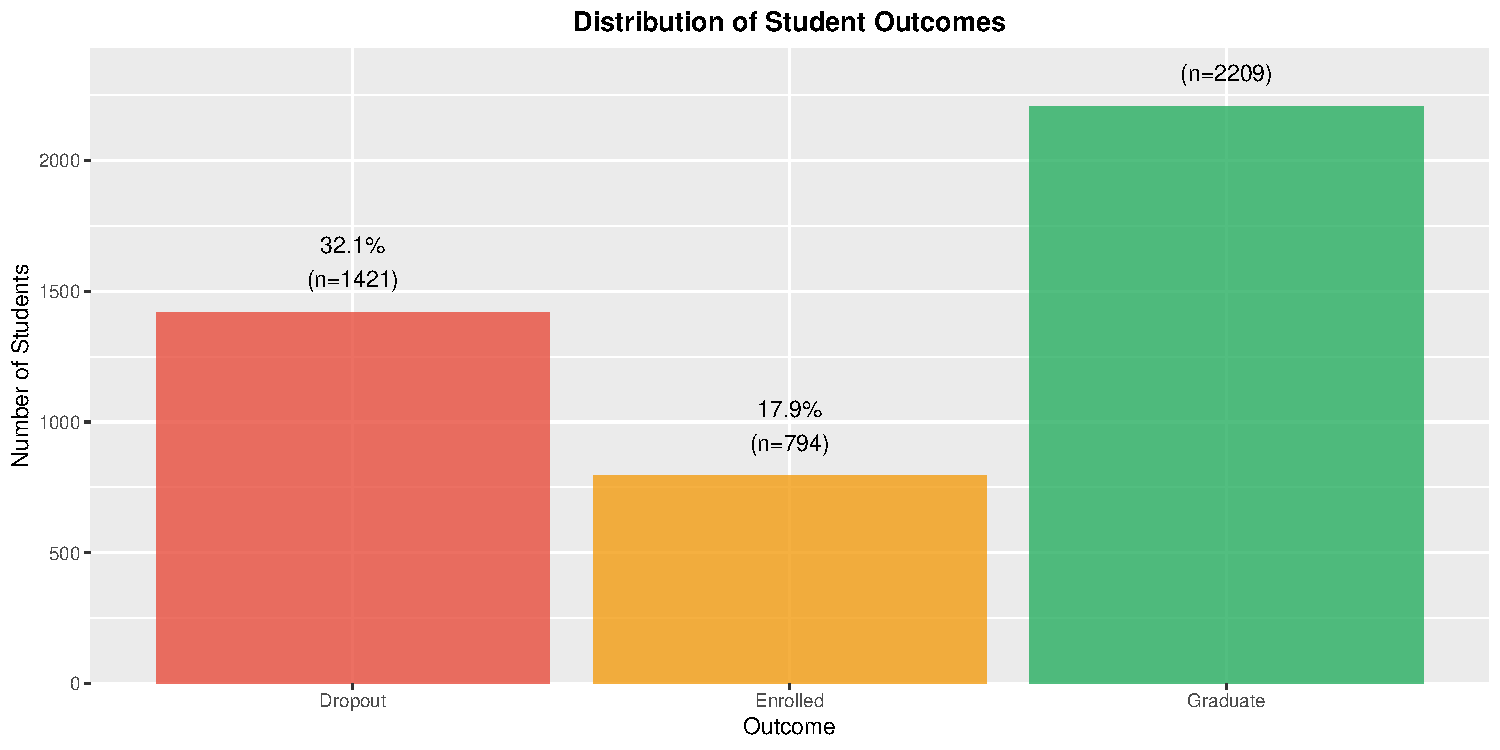
\includegraphics{final_report_ml1_group_files/figure-latex/target-distribution-1} \end{center}

\textbf{Key Observation:} The dataset shows a \emph{reasonable
distribution} for modeling, with 50\% graduates, 32\% dropouts, and 18\%
still enrolled. This balance allows models to learn patterns for all
outcomes effectively. Depending on the model and task, we may need to
\emph{adjust} the classes to \emph{binary(dropout or not dropout)}.

\subsection{2.2 First Semester Performance
Analysis}\label{first-semester-performance-analysis}

\begin{Shaded}
\begin{Highlighting}[]
\CommentTok{\# Prepare data for first semester grades}
\NormalTok{first\_sem\_data }\OtherTok{\textless{}{-}}\NormalTok{ df }\SpecialCharTok{\%\textgreater{}\%}
  \FunctionTok{filter}\NormalTok{(}\SpecialCharTok{!}\FunctionTok{is.na}\NormalTok{(Curricular.units}\FloatTok{.1}\NormalTok{st.sem..grade.) }\SpecialCharTok{\&}
\NormalTok{         Curricular.units}\FloatTok{.1}\NormalTok{st.sem..grade. }\SpecialCharTok{\textgreater{}} \DecValTok{0}\NormalTok{) }\SpecialCharTok{\%\textgreater{}\%}
  \FunctionTok{select}\NormalTok{(Target, Curricular.units}\FloatTok{.1}\NormalTok{st.sem..grade.,}
\NormalTok{         Curricular.units}\FloatTok{.1}\NormalTok{st.sem..approved.)}

\CommentTok{\# Box plot for first semester grades}
\NormalTok{p1 }\OtherTok{\textless{}{-}} \FunctionTok{ggplot}\NormalTok{(first\_sem\_data, }\FunctionTok{aes}\NormalTok{(}\AttributeTok{x =}\NormalTok{ Target, }\AttributeTok{y =}\NormalTok{ Curricular.units}\FloatTok{.1}\NormalTok{st.sem..grade., }\AttributeTok{fill =}\NormalTok{ Target)) }\SpecialCharTok{+}
  \FunctionTok{geom\_boxplot}\NormalTok{(}\AttributeTok{alpha =} \FloatTok{0.7}\NormalTok{) }\SpecialCharTok{+}
  \FunctionTok{scale\_fill\_manual}\NormalTok{(}\AttributeTok{values =} \FunctionTok{c}\NormalTok{(}\StringTok{"Dropout"} \OtherTok{=} \StringTok{"\#E74C3C"}\NormalTok{,}
                                \StringTok{"Enrolled"} \OtherTok{=} \StringTok{"\#F39C12"}\NormalTok{,}
                                \StringTok{"Graduate"} \OtherTok{=} \StringTok{"\#27AE60"}\NormalTok{)) }\SpecialCharTok{+}
  \FunctionTok{labs}\NormalTok{(}\AttributeTok{title =} \StringTok{"First Semester Grades by Outcome"}\NormalTok{,}
       \AttributeTok{x =} \StringTok{"Outcome"}\NormalTok{, }\AttributeTok{y =} \StringTok{"First Semester Grade (0{-}20)"}\NormalTok{) }\SpecialCharTok{+}
  \FunctionTok{theme}\NormalTok{(}\AttributeTok{legend.position =} \StringTok{"none"}\NormalTok{)}

\CommentTok{\# Box plot for courses approved}
\NormalTok{p2 }\OtherTok{\textless{}{-}} \FunctionTok{ggplot}\NormalTok{(first\_sem\_data, }\FunctionTok{aes}\NormalTok{(}\AttributeTok{x =}\NormalTok{ Target, }\AttributeTok{y =}\NormalTok{ Curricular.units}\FloatTok{.1}\NormalTok{st.sem..approved., }\AttributeTok{fill =}\NormalTok{ Target)) }\SpecialCharTok{+}
  \FunctionTok{geom\_boxplot}\NormalTok{(}\AttributeTok{alpha =} \FloatTok{0.7}\NormalTok{) }\SpecialCharTok{+}
  \FunctionTok{scale\_fill\_manual}\NormalTok{(}\AttributeTok{values =} \FunctionTok{c}\NormalTok{(}\StringTok{"Dropout"} \OtherTok{=} \StringTok{"\#E74C3C"}\NormalTok{,}
                                \StringTok{"Enrolled"} \OtherTok{=} \StringTok{"\#F39C12"}\NormalTok{,}
                                \StringTok{"Graduate"} \OtherTok{=} \StringTok{"\#27AE60"}\NormalTok{)) }\SpecialCharTok{+}
  \FunctionTok{labs}\NormalTok{(}\AttributeTok{title =} \StringTok{"Courses Approved in First Semester"}\NormalTok{,}
       \AttributeTok{x =} \StringTok{"Outcome"}\NormalTok{, }\AttributeTok{y =} \StringTok{"Number of Courses Approved"}\NormalTok{) }\SpecialCharTok{+}
  \FunctionTok{theme}\NormalTok{(}\AttributeTok{legend.position =} \StringTok{"none"}\NormalTok{)}

\FunctionTok{grid.arrange}\NormalTok{(p1, p2, }\AttributeTok{ncol =} \DecValTok{2}\NormalTok{)}
\end{Highlighting}
\end{Shaded}

\begin{center}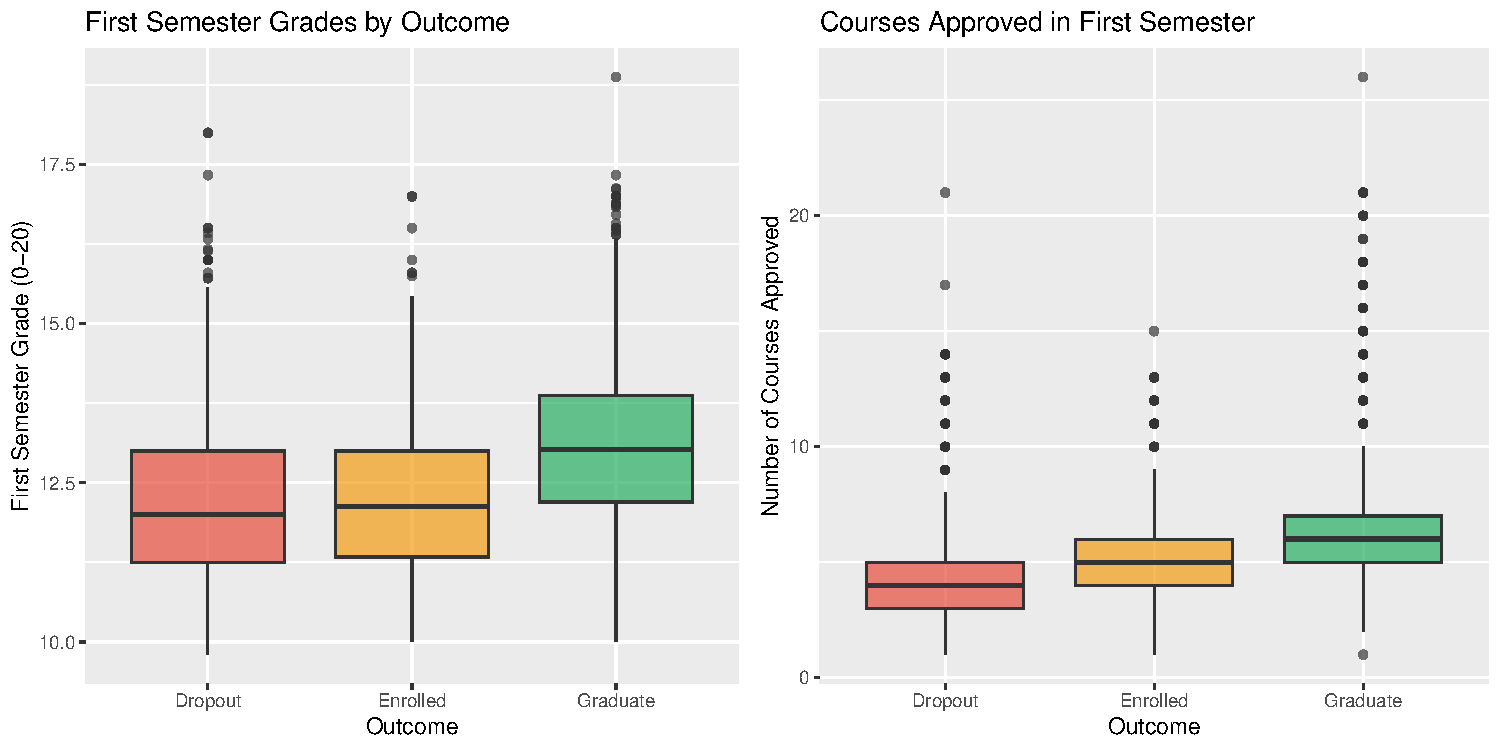
\includegraphics{final_report_ml1_group_files/figure-latex/first-sem-analysis-1} \end{center}

\textbf{Insight:} \emph{First semester performance} shows dramatic
differences across outcomes. Graduate students average \textbf{13+ grade
points} and complete most enrolled courses(approved), while dropout
students struggle with grades around \textbf{9-10} and complete fewer
courses. This suggests that first semester performance \emph{could be a
critical indicator} for dropout prediction.

\subsection{2.3 Financial \& Socioeconomic
Factors}\label{financial-socioeconomic-factors}

\begin{Shaded}
\begin{Highlighting}[]
\CommentTok{\# Prepare financial data}
\NormalTok{financial\_data }\OtherTok{\textless{}{-}}\NormalTok{ df }\SpecialCharTok{\%\textgreater{}\%}
  \FunctionTok{select}\NormalTok{(Target, Tuition.fees.up.to.date, Scholarship.holder, Debtor) }\SpecialCharTok{\%\textgreater{}\%}
  \FunctionTok{mutate}\NormalTok{(}\AttributeTok{Tuition.fees.up.to.date =} \FunctionTok{factor}\NormalTok{(Tuition.fees.up.to.date,}
                                           \AttributeTok{levels =} \FunctionTok{c}\NormalTok{(}\DecValTok{0}\NormalTok{, }\DecValTok{1}\NormalTok{),}
                                           \AttributeTok{labels =} \FunctionTok{c}\NormalTok{(}\StringTok{"Not Current"}\NormalTok{, }\StringTok{"Current"}\NormalTok{)),}
         \AttributeTok{Scholarship.holder =} \FunctionTok{factor}\NormalTok{(Scholarship.holder,}
                                     \AttributeTok{levels =} \FunctionTok{c}\NormalTok{(}\DecValTok{0}\NormalTok{, }\DecValTok{1}\NormalTok{),}
                                     \AttributeTok{labels =} \FunctionTok{c}\NormalTok{(}\StringTok{"No"}\NormalTok{, }\StringTok{"Yes"}\NormalTok{)),}
         \AttributeTok{Debtor =} \FunctionTok{factor}\NormalTok{(Debtor,}
                        \AttributeTok{levels =} \FunctionTok{c}\NormalTok{(}\DecValTok{0}\NormalTok{, }\DecValTok{1}\NormalTok{),}
                        \AttributeTok{labels =} \FunctionTok{c}\NormalTok{(}\StringTok{"No"}\NormalTok{, }\StringTok{"Yes"}\NormalTok{)))}

\CommentTok{\# Tuition status}
\NormalTok{p1 }\OtherTok{\textless{}{-}} \FunctionTok{ggplot}\NormalTok{(financial\_data, }\FunctionTok{aes}\NormalTok{(}\AttributeTok{x =}\NormalTok{ Tuition.fees.up.to.date, }\AttributeTok{fill =}\NormalTok{ Target)) }\SpecialCharTok{+}
  \FunctionTok{geom\_bar}\NormalTok{(}\AttributeTok{position =} \StringTok{"fill"}\NormalTok{) }\SpecialCharTok{+}
  \FunctionTok{scale\_fill\_manual}\NormalTok{(}\AttributeTok{values =} \FunctionTok{c}\NormalTok{(}\StringTok{"Dropout"} \OtherTok{=} \StringTok{"\#E74C3C"}\NormalTok{,}
                                \StringTok{"Enrolled"} \OtherTok{=} \StringTok{"\#F39C12"}\NormalTok{,}
                                \StringTok{"Graduate"} \OtherTok{=} \StringTok{"\#27AE60"}\NormalTok{)) }\SpecialCharTok{+}
  \FunctionTok{labs}\NormalTok{(}\AttributeTok{title =} \StringTok{"Tuition Payment Status"}\NormalTok{,}
       \AttributeTok{x =} \StringTok{"Tuition Fees Status"}\NormalTok{, }\AttributeTok{y =} \StringTok{"Proportion"}\NormalTok{, }\AttributeTok{fill =} \StringTok{"Outcome"}\NormalTok{)}

\CommentTok{\# Scholarship status}
\NormalTok{p2 }\OtherTok{\textless{}{-}} \FunctionTok{ggplot}\NormalTok{(financial\_data, }\FunctionTok{aes}\NormalTok{(}\AttributeTok{x =}\NormalTok{ Scholarship.holder, }\AttributeTok{fill =}\NormalTok{ Target)) }\SpecialCharTok{+}
  \FunctionTok{geom\_bar}\NormalTok{(}\AttributeTok{position =} \StringTok{"fill"}\NormalTok{) }\SpecialCharTok{+}
  \FunctionTok{scale\_fill\_manual}\NormalTok{(}\AttributeTok{values =} \FunctionTok{c}\NormalTok{(}\StringTok{"Dropout"} \OtherTok{=} \StringTok{"\#E74C3C"}\NormalTok{,}
                                \StringTok{"Enrolled"} \OtherTok{=} \StringTok{"\#F39C12"}\NormalTok{,}
                                \StringTok{"Graduate"} \OtherTok{=} \StringTok{"\#27AE60"}\NormalTok{)) }\SpecialCharTok{+}
  \FunctionTok{labs}\NormalTok{(}\AttributeTok{title =} \StringTok{"Scholarship Holder Status"}\NormalTok{,}
       \AttributeTok{x =} \StringTok{"Has Scholarship"}\NormalTok{, }\AttributeTok{y =} \StringTok{"Proportion"}\NormalTok{, }\AttributeTok{fill =} \StringTok{"Outcome"}\NormalTok{)}

\FunctionTok{grid.arrange}\NormalTok{(p1, p2, }\AttributeTok{ncol =} \DecValTok{2}\NormalTok{)}
\end{Highlighting}
\end{Shaded}

\begin{center}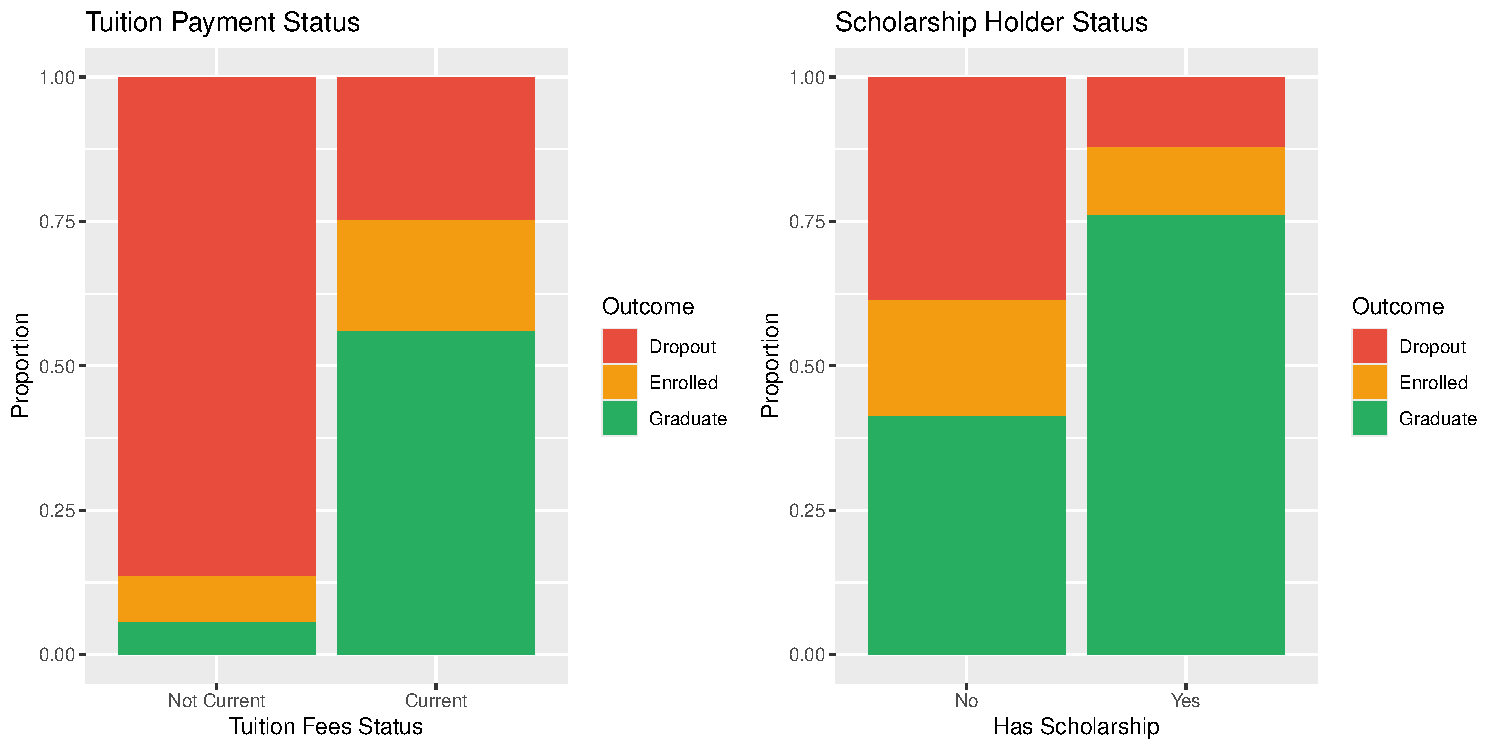
\includegraphics{final_report_ml1_group_files/figure-latex/financial-factors-1} \end{center}

\textbf{Insight:} Students that currently \emph{pays tuition on
time}(tuition.fees.up.to.date) show significantly higher graduation
rates. Scholarship holders also demonstrate better outcomes, suggesting
that financial situation could play an important role in student
success.

\subsection{2.4 Age Distribution}\label{age-distribution}

\begin{Shaded}
\begin{Highlighting}[]
\FunctionTok{ggplot}\NormalTok{(df, }\FunctionTok{aes}\NormalTok{(}\AttributeTok{x =}\NormalTok{ Age.at.enrollment, }\AttributeTok{fill =}\NormalTok{ Target)) }\SpecialCharTok{+}
  \FunctionTok{geom\_density}\NormalTok{(}\AttributeTok{alpha =} \FloatTok{0.6}\NormalTok{) }\SpecialCharTok{+}
  \FunctionTok{scale\_fill\_manual}\NormalTok{(}\AttributeTok{values =} \FunctionTok{c}\NormalTok{(}\StringTok{"Dropout"} \OtherTok{=} \StringTok{"\#E74C3C"}\NormalTok{,}
                                \StringTok{"Enrolled"} \OtherTok{=} \StringTok{"\#F39C12"}\NormalTok{,}
                                \StringTok{"Graduate"} \OtherTok{=} \StringTok{"\#27AE60"}\NormalTok{)) }\SpecialCharTok{+}
  \FunctionTok{labs}\NormalTok{(}\AttributeTok{title =} \StringTok{"Age Distribution by Student Outcome"}\NormalTok{,}
       \AttributeTok{x =} \StringTok{"Age at Enrollment"}\NormalTok{, }\AttributeTok{y =} \StringTok{"Density"}\NormalTok{, }\AttributeTok{fill =} \StringTok{"Outcome"}\NormalTok{) }\SpecialCharTok{+}
  \FunctionTok{theme}\NormalTok{(}\AttributeTok{legend.position =} \StringTok{"bottom"}\NormalTok{)}
\end{Highlighting}
\end{Shaded}

\begin{center}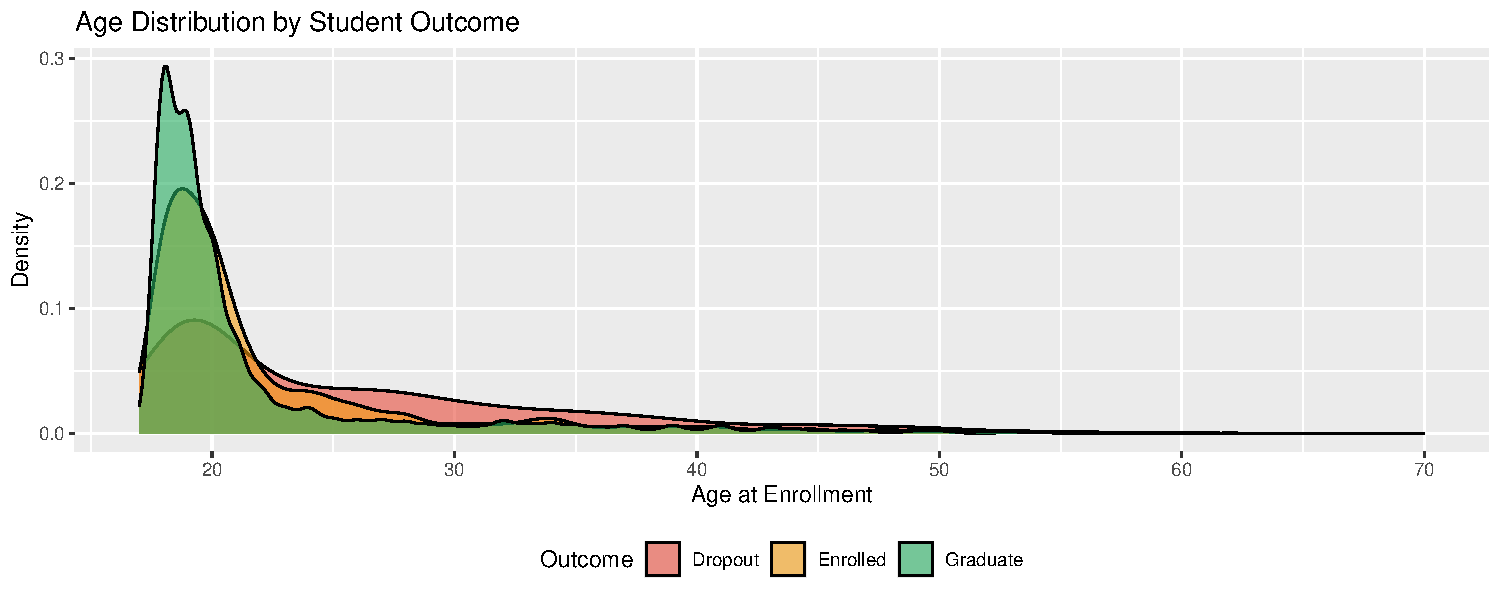
\includegraphics{final_report_ml1_group_files/figure-latex/age-distribution-1} \end{center}

\textbf{Insight:} Age shows interesting patterns: common students age
\emph{(18-22)} have \emph{higher graduation rates}, while both younger
and significantly older students face elevated dropout risks. This
pattern suggests that age effects may not follow a linear trend, which
we could explore using models that can capture such relationships (e.g.,
\emph{GAMs} with smooth terms, or GLMs with \emph{polynomial/spline}
features).

\begin{center}\rule{0.5\linewidth}{0.5pt}\end{center}

\section{3. Modeling Approach \&
Strategy}\label{modeling-approach-strategy}

\subsection{3.1 Model Characteristics}\label{model-characteristics}

We employ six modeling techniques, each with distinct strengths:

{\def\LTcaptype{none} % do not increment counter
\begin{longtable}[]{@{}
  >{\raggedright\arraybackslash}p{(\linewidth - 4\tabcolsep) * \real{0.2500}}
  >{\raggedright\arraybackslash}p{(\linewidth - 4\tabcolsep) * \real{0.3056}}
  >{\raggedright\arraybackslash}p{(\linewidth - 4\tabcolsep) * \real{0.4444}}@{}}
\toprule\noalign{}
\begin{minipage}[b]{\linewidth}\raggedright
Model
\end{minipage} & \begin{minipage}[b]{\linewidth}\raggedright
Purpose
\end{minipage} & \begin{minipage}[b]{\linewidth}\raggedright
Strengths
\end{minipage} \\
\midrule\noalign{}
\endhead
\bottomrule\noalign{}
\endlastfoot
\textbf{Linear Regression} & Predict continuous grades & Interpretable,
fast, baseline for comparison \\
\textbf{GLM (Binomial)} & Binary classification & Probabilistic output,
interpretable odds ratios \\
\textbf{GLM (Poisson)} & Count data prediction & Appropriate for
non-negative integer outcomes \\
\textbf{GAM} & Non-linear relationships & Captures curves, visualizable,
flexible \\
\textbf{Neural Networks} & Complex patterns & Learns interactions
automatically, high capacity \\
\textbf{SVM} & Robust classification & Maximum margin, kernel tricks,
outlier resistant \\
\end{longtable}
}

\subsection{3.2 Research Questions}\label{research-questions}

Each model addresses specific questions:

\begin{enumerate}
\def\labelenumi{\arabic{enumi}.}
\tightlist
\item
  \textbf{Linear Regression:} How do student characteristics linearly
  predict \textbf{second semester grades}?
\item
  \textbf{GLM (Binomial):} What factors distinguish \textbf{graduates
  from dropouts} in probabilistic terms?
\item
  \textbf{GLM (Poisson):} What predicts the \textbf{count of approved
  courses} in each semester?
\item
  \textbf{GAM:} Are there \textbf{non-linear relationships} that
  traditional linear models miss?
\item
  \textbf{Neural Networks:} Can \textbf{deep learning} uncover
  \textbf{hidden interaction patterns}?
\item
  \textbf{SVM:} Can we build a \textbf{robust classifier} that maximizes
  the margin between success and failure?
\end{enumerate}

\subsection{3.3 Evaluation Strategy}\label{evaluation-strategy}

\begin{itemize}
\tightlist
\item
  \textbf{Training/Test Split:} \textbf{80/20 stratified split} to
  maintain class balance
\item
  \textbf{Regression Metrics:} \textbf{R²}, \textbf{RMSE}, \textbf{MAE}
\item
  \textbf{Classification Metrics:} \textbf{Accuracy}, \textbf{AUC-ROC},
  \textbf{Confusion Matrix}
\item
  \textbf{Cross-Model Comparison:} Identify \textbf{consistent
  predictors} across methods
\end{itemize}

\begin{center}\rule{0.5\linewidth}{0.5pt}\end{center}

\section{4. Linear Regression
Analysis}\label{linear-regression-analysis}

\subsection{4.1 Introduction to the
Problem}\label{introduction-to-the-problem}

Predicting student grades is fundamental to early intervention
strategies. Linear regression provides an interpretable framework for
understanding how various factors---from prior academic preparation to
socioeconomic conditions---combine to influence academic performance.
While simple in concept, this approach reveals which factors matter most
and by how much.

\subsection{4.2 Methodology}\label{methodology}

Linear regression models the relationship between predictor variables
and a continuous outcome through the equation:

\[Y = \beta_0 + \beta_1X_1 + \beta_2X_2 + ... + \beta_nX_n + \epsilon\]

where \(Y\) represents second semester grades, \(X_i\) are our predictor
variables, \(\beta_i\) are coefficients indicating the strength and
direction of each relationship, and \(\epsilon\) captures random error.

We predict second semester grades based on 13 carefully selected
features including demographic factors, previous academic performance,
and economic indicators. This multi-factor approach recognizes that
student success results from the interplay of personal, academic, and
contextual variables.

\subsection{4.3 Data Preparation}\label{data-preparation}

\begin{Shaded}
\begin{Highlighting}[]
\NormalTok{TARGET }\OtherTok{\textless{}{-}} \StringTok{\textquotesingle{}Curricular.units.2nd.sem..grade.\textquotesingle{}}

\NormalTok{FEATURES }\OtherTok{\textless{}{-}} \FunctionTok{c}\NormalTok{(}
    \StringTok{\textquotesingle{}Previous.qualification..grade.\textquotesingle{}}\NormalTok{,}
    \StringTok{\textquotesingle{}Admission.grade\textquotesingle{}}\NormalTok{,}
    \StringTok{\textquotesingle{}Age.at.enrollment\textquotesingle{}}\NormalTok{,}
    \StringTok{"Mother.s.qualification"}\NormalTok{,}
    \StringTok{"Father.s.qualification"}\NormalTok{,}
    \StringTok{\textquotesingle{}Scholarship.holder\textquotesingle{}}\NormalTok{,}
    \StringTok{\textquotesingle{}Curricular.units.1st.sem..credited.\textquotesingle{}}\NormalTok{,}
    \StringTok{\textquotesingle{}Curricular.units.1st.sem..enrolled.\textquotesingle{}}\NormalTok{,}
    \StringTok{\textquotesingle{}Curricular.units.1st.sem..approved.\textquotesingle{}}\NormalTok{,}
    \StringTok{\textquotesingle{}Curricular.units.1st.sem..grade.\textquotesingle{}}\NormalTok{,}
    \StringTok{\textquotesingle{}Unemployment.rate\textquotesingle{}}\NormalTok{,}
    \StringTok{\textquotesingle{}Inflation.rate\textquotesingle{}}\NormalTok{,}
    \StringTok{\textquotesingle{}GDP\textquotesingle{}}
\NormalTok{)}

\NormalTok{df\_model }\OtherTok{\textless{}{-}}\NormalTok{ df }\SpecialCharTok{\%\textgreater{}\%}
    \FunctionTok{select}\NormalTok{(}\FunctionTok{all\_of}\NormalTok{(}\FunctionTok{c}\NormalTok{(FEATURES, TARGET))) }\SpecialCharTok{\%\textgreater{}\%}
    \FunctionTok{mutate}\NormalTok{(}\FunctionTok{across}\NormalTok{(}\FunctionTok{everything}\NormalTok{(), }\SpecialCharTok{\textasciitilde{}} \FunctionTok{as.numeric}\NormalTok{(}\FunctionTok{as.character}\NormalTok{(.)))) }\SpecialCharTok{\%\textgreater{}\%}
    \FunctionTok{drop\_na}\NormalTok{() }\SpecialCharTok{\%\textgreater{}\%}
    \FunctionTok{filter}\NormalTok{(}\FunctionTok{get}\NormalTok{(TARGET) }\SpecialCharTok{\textgreater{}} \DecValTok{0}\NormalTok{)}
\end{Highlighting}
\end{Shaded}

After filtering missing values and excluding zero grades, the linear
regression model uses \textbf{3554 students}. The target variable
(\textbf{2nd semester grade}) has \textbf{mean} \textbf{12.73} and
\textbf{standard deviation} \textbf{1.38}.

The dataset is filtered to \textbf{exclude students with zero grades},
as these typically represent withdrawals or incomplete coursework rather
than actual performance. This ensures our model focuses on
\textbf{predicting outcomes for actively enrolled students}.

\subsection{4.4 Exploratory Analysis}\label{exploratory-analysis}

\begin{Shaded}
\begin{Highlighting}[]
\NormalTok{correlations }\OtherTok{\textless{}{-}} \FunctionTok{cor}\NormalTok{(df\_model[FEATURES], df\_model[[TARGET]])}
\NormalTok{correlations\_sorted }\OtherTok{\textless{}{-}} \FunctionTok{sort}\NormalTok{(correlations[,}\DecValTok{1}\NormalTok{], }\AttributeTok{decreasing =} \ConstantTok{TRUE}\NormalTok{)}

\NormalTok{top5\_cor }\OtherTok{\textless{}{-}} \FunctionTok{data.frame}\NormalTok{(}
  \AttributeTok{Feature =} \FunctionTok{names}\NormalTok{(}\FunctionTok{head}\NormalTok{(correlations\_sorted, }\DecValTok{5}\NormalTok{)),}
  \AttributeTok{Correlation =} \FunctionTok{as.numeric}\NormalTok{(}\FunctionTok{round}\NormalTok{(}\FunctionTok{head}\NormalTok{(correlations\_sorted, }\DecValTok{5}\NormalTok{), }\DecValTok{3}\NormalTok{))}
\NormalTok{)}

\NormalTok{knitr}\SpecialCharTok{::}\FunctionTok{kable}\NormalTok{(top5\_cor, }\AttributeTok{caption =} \StringTok{"Top 5 correlations with 2nd semester grade"}\NormalTok{)}
\end{Highlighting}
\end{Shaded}

\begin{longtable}[]{@{}lr@{}}
\caption{Top 5 correlations with 2nd semester grade}\tabularnewline
\toprule\noalign{}
Feature & Correlation \\
\midrule\noalign{}
\endfirsthead
\toprule\noalign{}
Feature & Correlation \\
\midrule\noalign{}
\endhead
\bottomrule\noalign{}
\endlastfoot
Curricular.units.1st.sem..grade. & 0.516 \\
Admission.grade & 0.276 \\
Curricular.units.1st.sem..approved. & 0.250 \\
Previous.qualification..grade. & 0.249 \\
Scholarship.holder & 0.102 \\
\end{longtable}

\subsubsection{Feature Relationships}\label{feature-relationships}

\begin{Shaded}
\begin{Highlighting}[]
\NormalTok{correlation\_matrix }\OtherTok{\textless{}{-}} \FunctionTok{cor}\NormalTok{(df\_model[}\FunctionTok{c}\NormalTok{(FEATURES, TARGET)])}

\FunctionTok{corrplot}\NormalTok{(correlation\_matrix,}
         \AttributeTok{method =} \StringTok{"color"}\NormalTok{,}
         \AttributeTok{type =} \StringTok{"upper"}\NormalTok{,}
         \AttributeTok{tl.col =} \StringTok{"black"}\NormalTok{,}
         \AttributeTok{tl.srt =} \DecValTok{45}\NormalTok{,}
         \AttributeTok{tl.cex =} \FloatTok{0.7}\NormalTok{,}
         \AttributeTok{col =} \FunctionTok{colorRampPalette}\NormalTok{(}\FunctionTok{c}\NormalTok{(}\StringTok{"blue"}\NormalTok{, }\StringTok{"white"}\NormalTok{, }\StringTok{"red"}\NormalTok{))(}\DecValTok{200}\NormalTok{),}
         \AttributeTok{addCoef.col =} \StringTok{"black"}\NormalTok{,}
         \AttributeTok{number.cex =} \FloatTok{0.4}\NormalTok{,}
         \AttributeTok{title =} \StringTok{"Feature Correlation Heatmap"}\NormalTok{,}
         \AttributeTok{mar =} \FunctionTok{c}\NormalTok{(}\DecValTok{0}\NormalTok{, }\DecValTok{0}\NormalTok{, }\DecValTok{2}\NormalTok{, }\DecValTok{0}\NormalTok{))}
\end{Highlighting}
\end{Shaded}

\begin{center}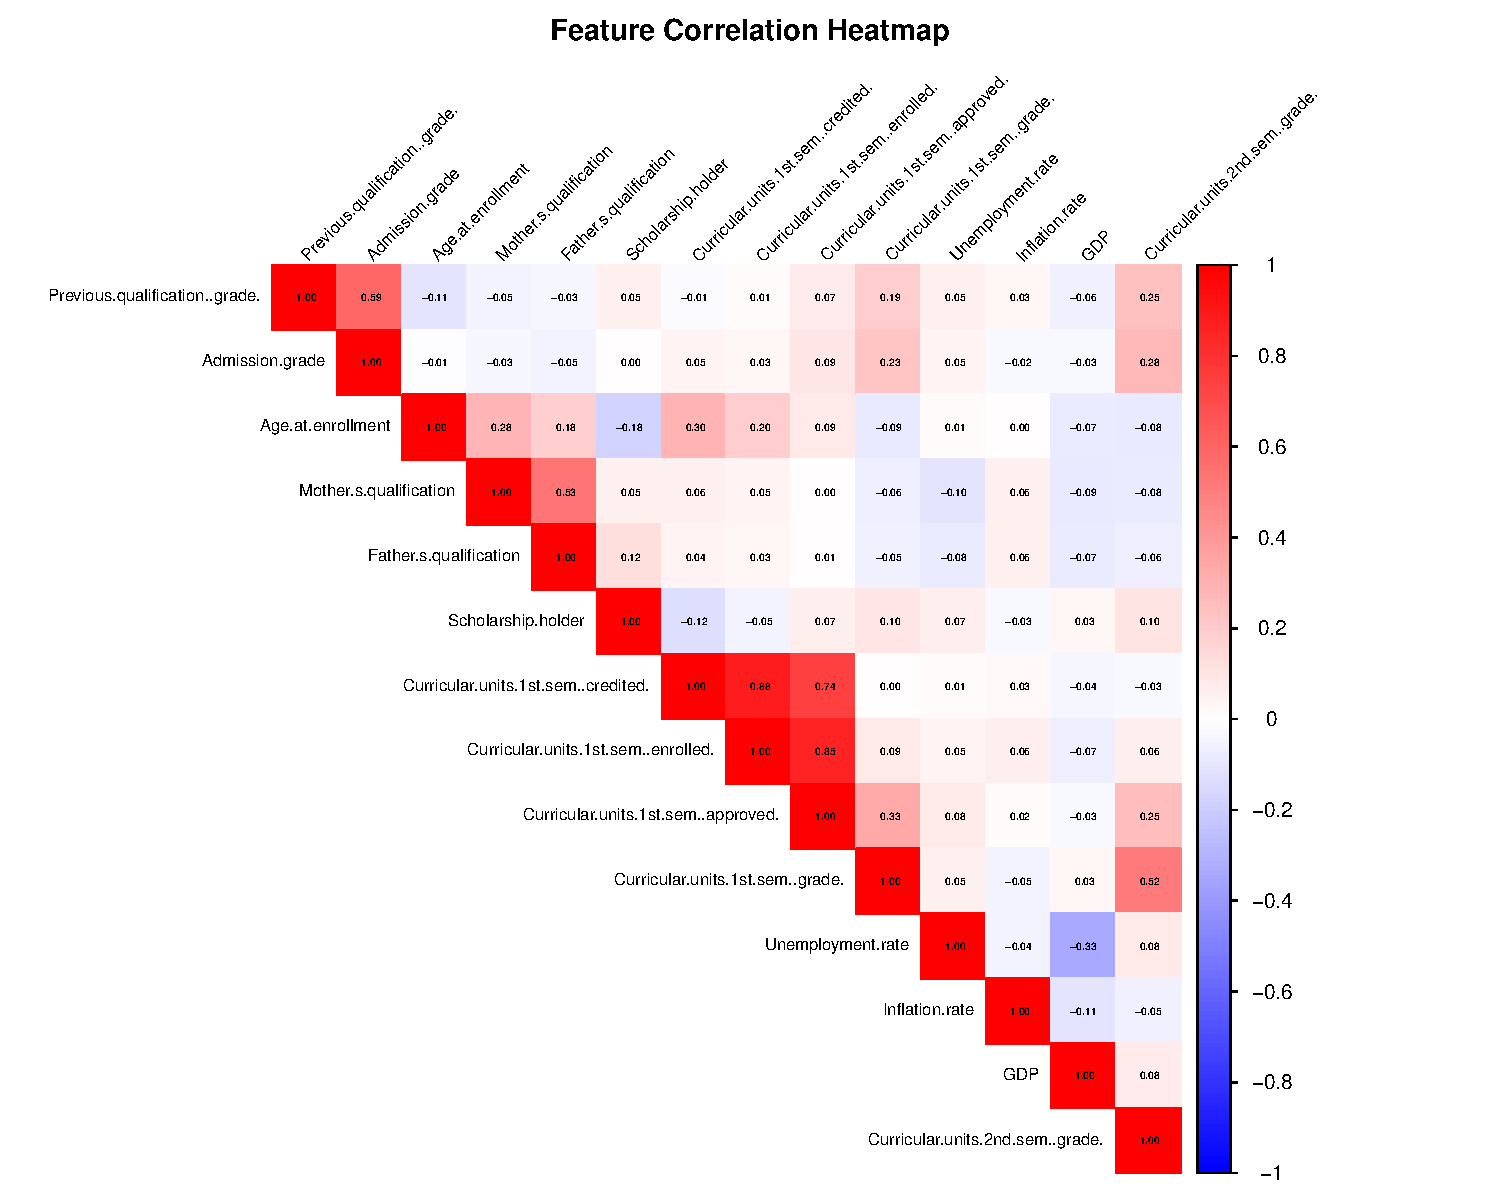
\includegraphics{final_report_ml1_group_files/figure-latex/linear-correlation-1} \end{center}

\textbf{Key Observations:} Strong positive correlations are evident
between \textbf{first semester performance metrics} and \textbf{second
semester grades}, suggesting that prior academic success is highly
predictive. This finding supports the importance of \textbf{early
intervention programs} targeting first-semester students.

\subsection{4.5 Model Development}\label{model-development}

\begin{Shaded}
\begin{Highlighting}[]
\FunctionTok{set.seed}\NormalTok{(}\DecValTok{42}\NormalTok{)}

\NormalTok{trainIndex }\OtherTok{\textless{}{-}} \FunctionTok{createDataPartition}\NormalTok{(df\_model[[TARGET]], }\AttributeTok{p =} \FloatTok{0.8}\NormalTok{, }\AttributeTok{list =} \ConstantTok{FALSE}\NormalTok{)}

\NormalTok{train\_data }\OtherTok{\textless{}{-}}\NormalTok{ df\_model[trainIndex, ]}
\NormalTok{test\_data }\OtherTok{\textless{}{-}}\NormalTok{ df\_model[}\SpecialCharTok{{-}}\NormalTok{trainIndex, ]}

\NormalTok{X\_train }\OtherTok{\textless{}{-}}\NormalTok{ train\_data }\SpecialCharTok{\%\textgreater{}\%}\NormalTok{ dplyr}\SpecialCharTok{::}\FunctionTok{select}\NormalTok{(}\FunctionTok{all\_of}\NormalTok{(FEATURES))}
\NormalTok{y\_train }\OtherTok{\textless{}{-}}\NormalTok{ train\_data[[TARGET]]}
\NormalTok{X\_test }\OtherTok{\textless{}{-}}\NormalTok{ test\_data }\SpecialCharTok{\%\textgreater{}\%}\NormalTok{ dplyr}\SpecialCharTok{::}\FunctionTok{select}\NormalTok{(}\FunctionTok{all\_of}\NormalTok{(FEATURES))}
\NormalTok{y\_test }\OtherTok{\textless{}{-}}\NormalTok{ test\_data[[TARGET]]}

\NormalTok{train\_n }\OtherTok{\textless{}{-}} \FunctionTok{nrow}\NormalTok{(train\_data)}
\NormalTok{test\_n }\OtherTok{\textless{}{-}} \FunctionTok{nrow}\NormalTok{(test\_data)}
\end{Highlighting}
\end{Shaded}

We use an \textbf{80/20 train-test split}, resulting in \textbf{2844}
training observations and \textbf{710} test observations.

\begin{Shaded}
\begin{Highlighting}[]
\NormalTok{preProc }\OtherTok{\textless{}{-}} \FunctionTok{preProcess}\NormalTok{(X\_train, }\AttributeTok{method =} \FunctionTok{c}\NormalTok{(}\StringTok{"center"}\NormalTok{, }\StringTok{"scale"}\NormalTok{))}
\NormalTok{X\_train\_scaled }\OtherTok{\textless{}{-}} \FunctionTok{predict}\NormalTok{(preProc, X\_train)}
\NormalTok{X\_test\_scaled }\OtherTok{\textless{}{-}} \FunctionTok{predict}\NormalTok{(preProc, X\_test)}
\end{Highlighting}
\end{Shaded}

\textbf{Feature Scaling:} Standardization (\textbf{z-score
normalization}) ensures all features contribute proportionally to the
model regardless of their original scales.

\begin{longtable}[t]{>{}lr}
\caption{\label{tab:linear-train}Top 3 linear regression coefficients (by absolute value)}\\
\toprule
Feature & Coefficient\\
\midrule
\textbf{Curricular.units.1st.sem..grade.} & 0.5072096\\
\textbf{Curricular.units.1st.sem..approved.} & 0.3815536\\
\textbf{Curricular.units.1st.sem..credited.} & -0.3760881\\
\bottomrule
\end{longtable}

\subsection{4.6 Model Performance}\label{model-performance}

\begin{Shaded}
\begin{Highlighting}[]
\NormalTok{y\_train\_pred }\OtherTok{\textless{}{-}} \FunctionTok{predict}\NormalTok{(model, X\_train\_scaled)}
\NormalTok{y\_test\_pred }\OtherTok{\textless{}{-}} \FunctionTok{predict}\NormalTok{(model, X\_test\_scaled)}

\NormalTok{train\_r2 }\OtherTok{\textless{}{-}} \FunctionTok{cor}\NormalTok{(y\_train, y\_train\_pred)}\SpecialCharTok{\^{}}\DecValTok{2}
\NormalTok{train\_rmse }\OtherTok{\textless{}{-}} \FunctionTok{sqrt}\NormalTok{(}\FunctionTok{mean}\NormalTok{((y\_train }\SpecialCharTok{{-}}\NormalTok{ y\_train\_pred)}\SpecialCharTok{\^{}}\DecValTok{2}\NormalTok{))}
\NormalTok{train\_mae }\OtherTok{\textless{}{-}} \FunctionTok{mean}\NormalTok{(}\FunctionTok{abs}\NormalTok{(y\_train }\SpecialCharTok{{-}}\NormalTok{ y\_train\_pred))}

\NormalTok{test\_r2 }\OtherTok{\textless{}{-}} \FunctionTok{cor}\NormalTok{(y\_test, y\_test\_pred)}\SpecialCharTok{\^{}}\DecValTok{2}
\NormalTok{test\_rmse }\OtherTok{\textless{}{-}} \FunctionTok{sqrt}\NormalTok{(}\FunctionTok{mean}\NormalTok{((y\_test }\SpecialCharTok{{-}}\NormalTok{ y\_test\_pred)}\SpecialCharTok{\^{}}\DecValTok{2}\NormalTok{))}
\NormalTok{test\_mae }\OtherTok{\textless{}{-}} \FunctionTok{mean}\NormalTok{(}\FunctionTok{abs}\NormalTok{(y\_test }\SpecialCharTok{{-}}\NormalTok{ y\_test\_pred))}
\end{Highlighting}
\end{Shaded}

\textbf{Performance Interpretation:} The R² score of 0.372 indicates
that 37.2\% of variance in second semester grades can be explained by
our selected features. The Mean Absolute Error (MAE) of 0.86 means our
predictions are typically within 0.86 grade points of actual values.

\subsection{4.7 Visual Assessment}\label{visual-assessment}

\begin{Shaded}
\begin{Highlighting}[]
\FunctionTok{par}\NormalTok{(}\AttributeTok{mfrow =} \FunctionTok{c}\NormalTok{(}\DecValTok{1}\NormalTok{, }\DecValTok{2}\NormalTok{))}

\FunctionTok{plot}\NormalTok{(y\_train, y\_train\_pred,}
     \AttributeTok{xlab =} \StringTok{"Actual Grade"}\NormalTok{, }\AttributeTok{ylab =} \StringTok{"Predicted Grade"}\NormalTok{,}
     \AttributeTok{main =} \FunctionTok{sprintf}\NormalTok{(}\StringTok{"Training Set (R² = \%.4f)"}\NormalTok{, train\_r2),}
     \AttributeTok{pch =} \DecValTok{16}\NormalTok{, }\AttributeTok{col =} \FunctionTok{rgb}\NormalTok{(}\DecValTok{0}\NormalTok{, }\DecValTok{0}\NormalTok{, }\DecValTok{1}\NormalTok{, }\FloatTok{0.5}\NormalTok{))}
\FunctionTok{abline}\NormalTok{(}\AttributeTok{a =} \DecValTok{0}\NormalTok{, }\AttributeTok{b =} \DecValTok{1}\NormalTok{, }\AttributeTok{col =} \StringTok{"red"}\NormalTok{, }\AttributeTok{lwd =} \DecValTok{2}\NormalTok{, }\AttributeTok{lty =} \DecValTok{2}\NormalTok{)}
\FunctionTok{grid}\NormalTok{()}

\FunctionTok{plot}\NormalTok{(y\_test, y\_test\_pred,}
     \AttributeTok{xlab =} \StringTok{"Actual Grade"}\NormalTok{, }\AttributeTok{ylab =} \StringTok{"Predicted Grade"}\NormalTok{,}
     \AttributeTok{main =} \FunctionTok{sprintf}\NormalTok{(}\StringTok{"Test Set (R² = \%.4f)"}\NormalTok{, test\_r2),}
     \AttributeTok{pch =} \DecValTok{16}\NormalTok{, }\AttributeTok{col =} \FunctionTok{rgb}\NormalTok{(}\DecValTok{0}\NormalTok{, }\DecValTok{1}\NormalTok{, }\DecValTok{0}\NormalTok{, }\FloatTok{0.5}\NormalTok{))}
\FunctionTok{abline}\NormalTok{(}\AttributeTok{a =} \DecValTok{0}\NormalTok{, }\AttributeTok{b =} \DecValTok{1}\NormalTok{, }\AttributeTok{col =} \StringTok{"red"}\NormalTok{, }\AttributeTok{lwd =} \DecValTok{2}\NormalTok{, }\AttributeTok{lty =} \DecValTok{2}\NormalTok{)}
\FunctionTok{grid}\NormalTok{()}
\end{Highlighting}
\end{Shaded}

\begin{figure}

{\centering 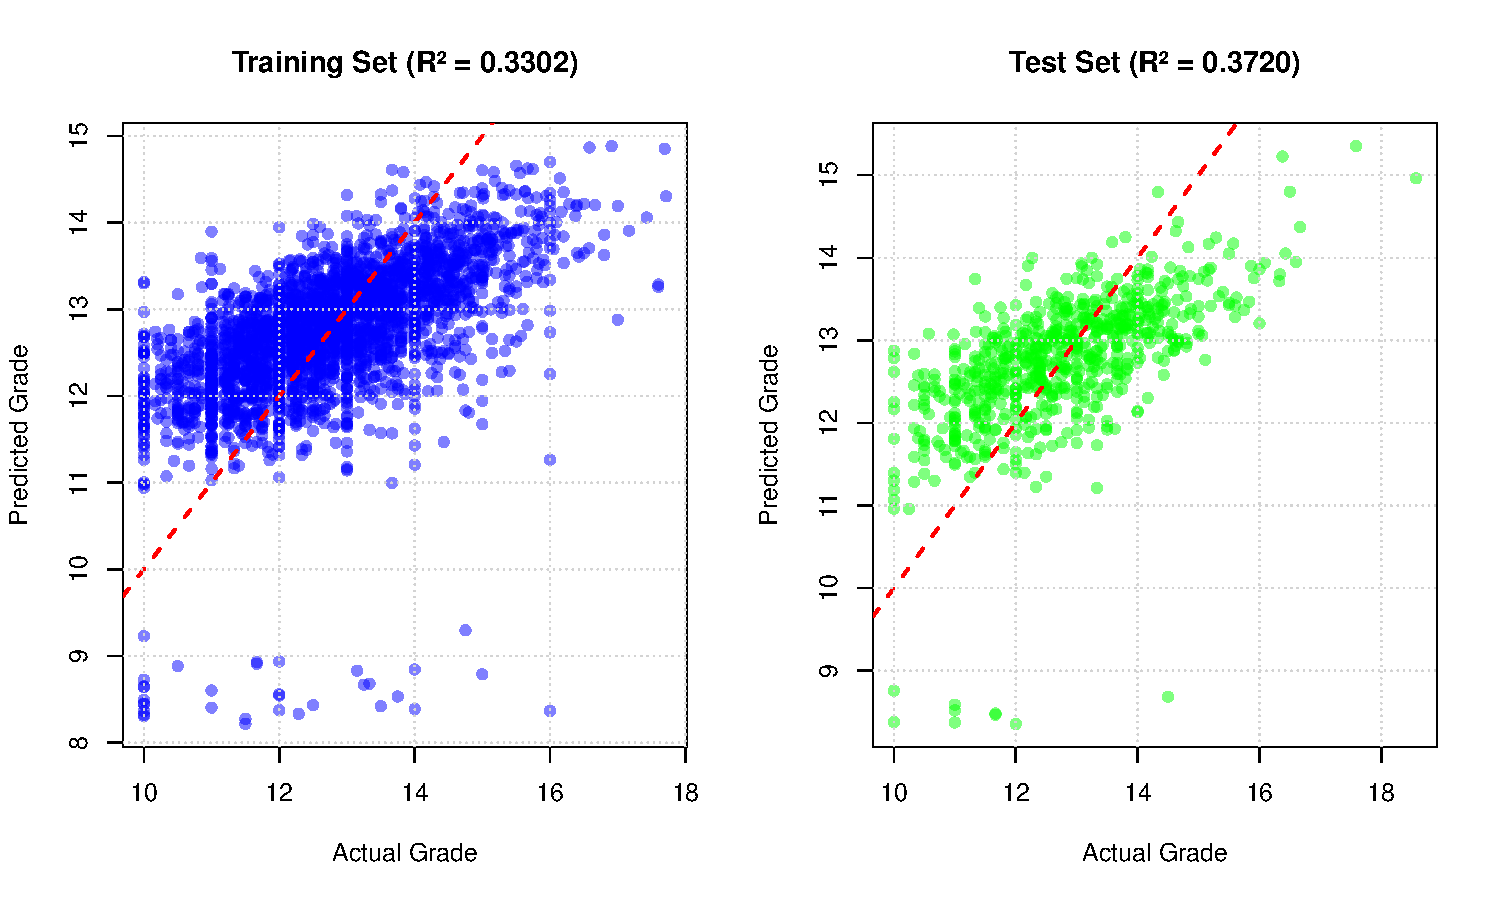
\includegraphics{final_report_ml1_group_files/figure-latex/linear-plots-1} 

}

\caption{Actual vs. Predicted Grades}\label{fig:linear-plots}
\end{figure}

\subsubsection{Residual Analysis}\label{residual-analysis}

\begin{Shaded}
\begin{Highlighting}[]
\NormalTok{residuals\_test }\OtherTok{\textless{}{-}}\NormalTok{ y\_test }\SpecialCharTok{{-}}\NormalTok{ y\_test\_pred}

\FunctionTok{par}\NormalTok{(}\AttributeTok{mfrow =} \FunctionTok{c}\NormalTok{(}\DecValTok{1}\NormalTok{, }\DecValTok{2}\NormalTok{))}

\FunctionTok{plot}\NormalTok{(y\_test\_pred, residuals\_test,}
     \AttributeTok{xlab =} \StringTok{"Predicted Grade"}\NormalTok{, }\AttributeTok{ylab =} \StringTok{"Residuals"}\NormalTok{,}
     \AttributeTok{main =} \StringTok{"Residual Plot"}\NormalTok{,}
     \AttributeTok{pch =} \DecValTok{16}\NormalTok{, }\AttributeTok{col =} \FunctionTok{rgb}\NormalTok{(}\DecValTok{0}\NormalTok{, }\DecValTok{0}\NormalTok{, }\DecValTok{1}\NormalTok{, }\FloatTok{0.5}\NormalTok{))}
\FunctionTok{abline}\NormalTok{(}\AttributeTok{h =} \DecValTok{0}\NormalTok{, }\AttributeTok{col =} \StringTok{"red"}\NormalTok{, }\AttributeTok{lwd =} \DecValTok{2}\NormalTok{, }\AttributeTok{lty =} \DecValTok{2}\NormalTok{)}
\FunctionTok{grid}\NormalTok{()}

\FunctionTok{hist}\NormalTok{(residuals\_test, }\AttributeTok{breaks =} \DecValTok{30}\NormalTok{,}
     \AttributeTok{xlab =} \StringTok{"Residuals"}\NormalTok{, }\AttributeTok{ylab =} \StringTok{"Frequency"}\NormalTok{,}
     \AttributeTok{main =} \StringTok{"Residual Distribution"}\NormalTok{,}
     \AttributeTok{col =} \FunctionTok{rgb}\NormalTok{(}\DecValTok{0}\NormalTok{, }\DecValTok{0}\NormalTok{, }\DecValTok{1}\NormalTok{, }\FloatTok{0.7}\NormalTok{), }\AttributeTok{border =} \StringTok{"black"}\NormalTok{)}
\FunctionTok{abline}\NormalTok{(}\AttributeTok{v =} \DecValTok{0}\NormalTok{, }\AttributeTok{col =} \StringTok{"red"}\NormalTok{, }\AttributeTok{lwd =} \DecValTok{2}\NormalTok{, }\AttributeTok{lty =} \DecValTok{2}\NormalTok{)}
\FunctionTok{grid}\NormalTok{()}
\end{Highlighting}
\end{Shaded}

\begin{figure}

{\centering 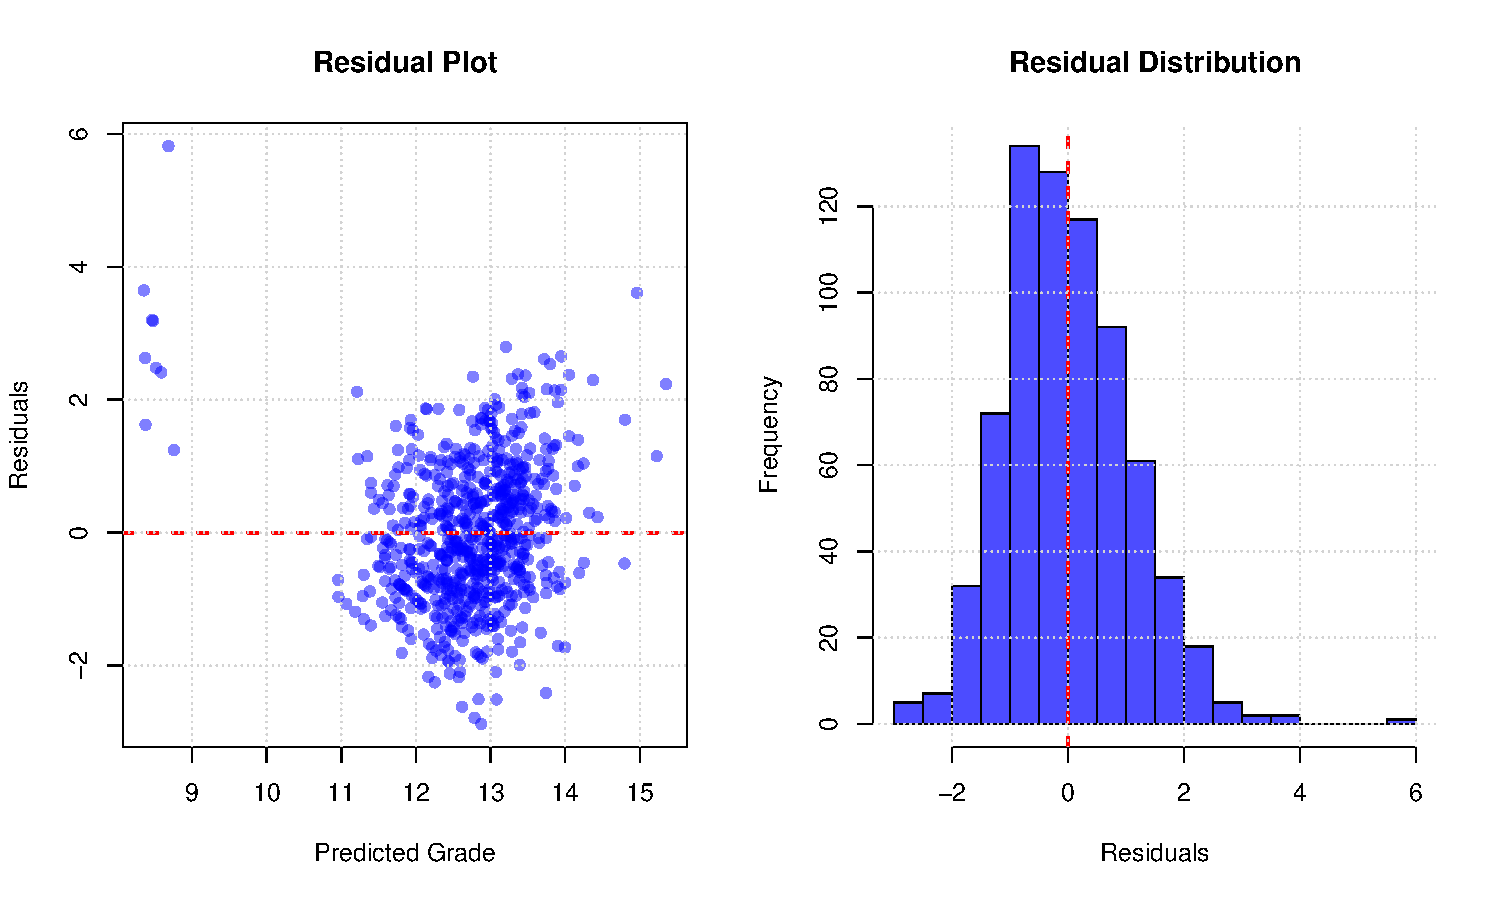
\includegraphics{final_report_ml1_group_files/figure-latex/linear-residuals-1} 

}

\caption{Residual diagnostics}\label{fig:linear-residuals}
\end{figure}

\subsection{4.8 Feature Importance}\label{feature-importance}

\begin{Shaded}
\begin{Highlighting}[]
\NormalTok{feature\_importance }\OtherTok{\textless{}{-}} \FunctionTok{data.frame}\NormalTok{(}
    \AttributeTok{Feature =} \FunctionTok{names}\NormalTok{(}\FunctionTok{coef}\NormalTok{(model))[}\SpecialCharTok{{-}}\DecValTok{1}\NormalTok{],}
    \AttributeTok{Coefficient =} \FunctionTok{coef}\NormalTok{(model)[}\SpecialCharTok{{-}}\DecValTok{1}\NormalTok{]}
\NormalTok{) }\SpecialCharTok{\%\textgreater{}\%}
    \FunctionTok{mutate}\NormalTok{(}\AttributeTok{Abs\_Coefficient =} \FunctionTok{abs}\NormalTok{(Coefficient)) }\SpecialCharTok{\%\textgreater{}\%}
    \FunctionTok{arrange}\NormalTok{(}\FunctionTok{desc}\NormalTok{(Abs\_Coefficient))}

\FunctionTok{par}\NormalTok{(}\AttributeTok{mar =} \FunctionTok{c}\NormalTok{(}\DecValTok{5}\NormalTok{, }\DecValTok{12}\NormalTok{, }\DecValTok{4}\NormalTok{, }\DecValTok{2}\NormalTok{))}
\NormalTok{colors }\OtherTok{\textless{}{-}} \FunctionTok{ifelse}\NormalTok{(feature\_importance}\SpecialCharTok{$}\NormalTok{Coefficient }\SpecialCharTok{\textgreater{}} \DecValTok{0}\NormalTok{, }\StringTok{"green"}\NormalTok{, }\StringTok{"red"}\NormalTok{)}
\FunctionTok{barplot}\NormalTok{(feature\_importance}\SpecialCharTok{$}\NormalTok{Coefficient,}
        \AttributeTok{names.arg =}\NormalTok{ feature\_importance}\SpecialCharTok{$}\NormalTok{Feature,}
        \AttributeTok{horiz =} \ConstantTok{TRUE}\NormalTok{,}
        \AttributeTok{las =} \DecValTok{1}\NormalTok{,}
        \AttributeTok{col =} \FunctionTok{adjustcolor}\NormalTok{(colors, }\AttributeTok{alpha.f =} \FloatTok{0.7}\NormalTok{),}
        \AttributeTok{xlab =} \StringTok{"Coefficient Value (Standardized)"}\NormalTok{,}
        \AttributeTok{main =} \StringTok{"Feature Importance in Grade Prediction"}\NormalTok{,}
        \AttributeTok{xlim =} \FunctionTok{c}\NormalTok{(}\FunctionTok{min}\NormalTok{(feature\_importance}\SpecialCharTok{$}\NormalTok{Coefficient) }\SpecialCharTok{*} \FloatTok{1.2}\NormalTok{,}
                 \FunctionTok{max}\NormalTok{(feature\_importance}\SpecialCharTok{$}\NormalTok{Coefficient) }\SpecialCharTok{*} \FloatTok{1.2}\NormalTok{))}
\FunctionTok{abline}\NormalTok{(}\AttributeTok{v =} \DecValTok{0}\NormalTok{, }\AttributeTok{col =} \StringTok{"black"}\NormalTok{, }\AttributeTok{lwd =} \DecValTok{1}\NormalTok{)}
\FunctionTok{grid}\NormalTok{()}
\end{Highlighting}
\end{Shaded}

\begin{figure}

{\centering 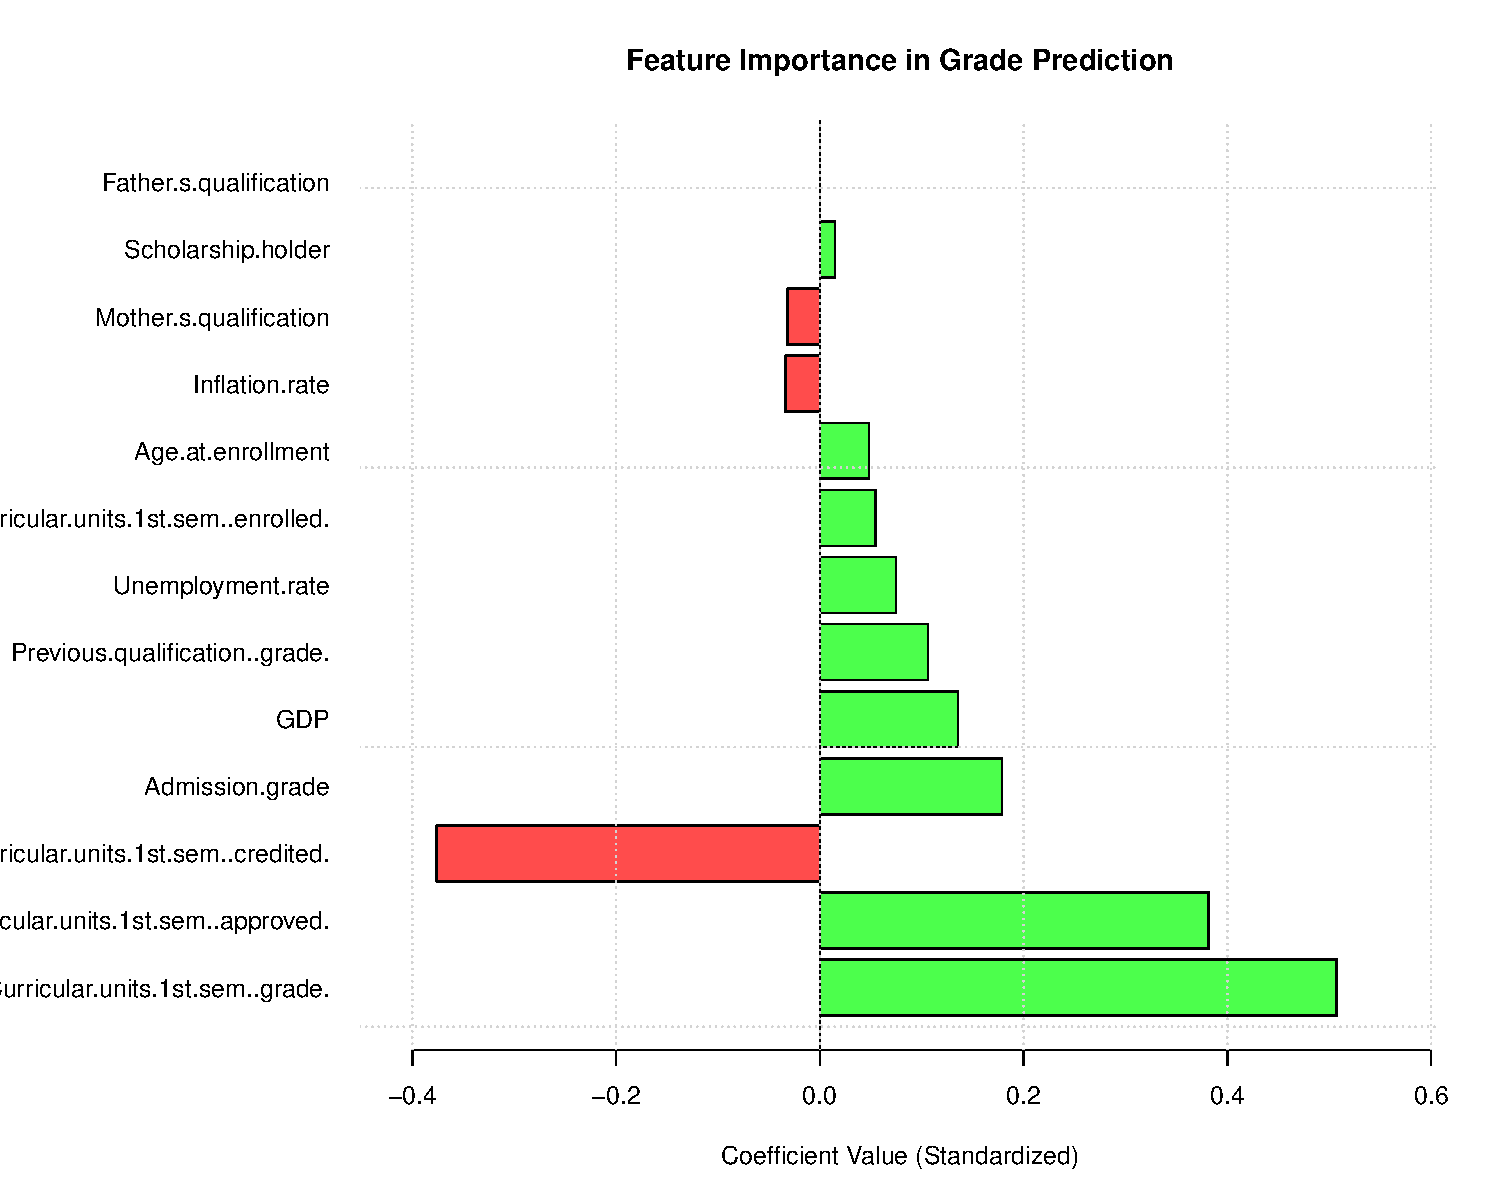
\includegraphics{final_report_ml1_group_files/figure-latex/linear-importance-1} 

}

\caption{Feature importance}\label{fig:linear-importance}
\end{figure}

\textbf{Key Insights:} First semester grades have the strongest positive
effect---students who perform well initially tend to continue
succeeding. Course approvals and enrollments in the first semester
significantly impact second semester outcomes. Economic indicators show
measurable but smaller effects.

\begin{center}\rule{0.5\linewidth}{0.5pt}\end{center}

\section{5. Generalized Linear Model -
Binomial}\label{generalized-linear-model---binomial}

\subsection{5.1 Introduction to
Classification}\label{introduction-to-classification}

Classification problems require predicting categorical outcomes rather
than continuous values. Binomial logistic regression excels at binary
classification by estimating probabilities between 0 and 1 through the
logistic (sigmoid) function:

\[P(Y=1) = \frac{1}{1 + e^{-(\beta_0 + \beta_1X_1 + ... + \beta_nX_n)}}\]

This S-shaped curve ensures predictions stay within valid probability
bounds while allowing us to model how predictor variables influence the
odds of an outcome.

\subsection{5.2 Model 1: Predicting High vs Low Admission
Scores}\label{model-1-predicting-high-vs-low-admission-scores}

Understanding what characteristics lead to high admission scores helps
institutions identify strong candidates and understand enrollment
patterns.

\subsubsection{Binomial GLM Pre-processing: High vs Low
Admission}\label{binomial-glm-pre-processing-high-vs-low-admission}

We convert \texttt{Admission.grade} into a binary target (\textbf{High}
vs \textbf{Low} admission) using the median cutoff (\textbf{126.1}).
After removing missing values, we model \textbf{4424} students.

\subsubsection{Model Performance}\label{model-performance-1}

\begin{Shaded}
\begin{Highlighting}[]
\NormalTok{pred\_adm\_prob }\OtherTok{\textless{}{-}} \FunctionTok{predict}\NormalTok{(glm\_adm, test\_adm\_scaled, }\AttributeTok{type =} \StringTok{"response"}\NormalTok{)}
\NormalTok{pred\_adm }\OtherTok{\textless{}{-}} \FunctionTok{ifelse}\NormalTok{(pred\_adm\_prob }\SpecialCharTok{\textgreater{}} \FloatTok{0.5}\NormalTok{, }\DecValTok{1}\NormalTok{, }\DecValTok{0}\NormalTok{)}

\NormalTok{accuracy\_adm }\OtherTok{\textless{}{-}} \FunctionTok{mean}\NormalTok{(pred\_adm }\SpecialCharTok{==}\NormalTok{ test\_adm\_scaled}\SpecialCharTok{$}\NormalTok{High\_Admission)}

\FunctionTok{cat}\NormalTok{(}\FunctionTok{sprintf}\NormalTok{(}\StringTok{"Binomial GLM (Admission) accuracy: \%.4f (\%.2f\%\%)}\SpecialCharTok{\textbackslash{}n}\StringTok{"}\NormalTok{, accuracy\_adm, accuracy\_adm }\SpecialCharTok{*} \DecValTok{100}\NormalTok{))}

\NormalTok{cm\_adm }\OtherTok{\textless{}{-}} \FunctionTok{confusionMatrix}\NormalTok{(}\FunctionTok{factor}\NormalTok{(pred\_adm, }\AttributeTok{levels =} \FunctionTok{c}\NormalTok{(}\DecValTok{0}\NormalTok{, }\DecValTok{1}\NormalTok{)),}
                          \FunctionTok{factor}\NormalTok{(test\_adm\_scaled}\SpecialCharTok{$}\NormalTok{High\_Admission, }\AttributeTok{levels =} \FunctionTok{c}\NormalTok{(}\DecValTok{0}\NormalTok{, }\DecValTok{1}\NormalTok{)))}
\FunctionTok{print}\NormalTok{(cm\_adm)}

\CommentTok{\# Confusion matrix plot}
\NormalTok{cm\_plot\_df }\OtherTok{\textless{}{-}} \FunctionTok{as.data.frame}\NormalTok{(cm\_adm}\SpecialCharTok{$}\NormalTok{table)}
\FunctionTok{names}\NormalTok{(cm\_plot\_df) }\OtherTok{\textless{}{-}} \FunctionTok{c}\NormalTok{(}\StringTok{"Prediction"}\NormalTok{, }\StringTok{"Reference"}\NormalTok{, }\StringTok{"Freq"}\NormalTok{)}
\NormalTok{cm\_plot\_df}\SpecialCharTok{$}\NormalTok{Prediction }\OtherTok{\textless{}{-}} \FunctionTok{factor}\NormalTok{(cm\_plot\_df}\SpecialCharTok{$}\NormalTok{Prediction, }\AttributeTok{levels =} \FunctionTok{c}\NormalTok{(}\StringTok{"0"}\NormalTok{, }\StringTok{"1"}\NormalTok{))}
\NormalTok{cm\_plot\_df}\SpecialCharTok{$}\NormalTok{Reference }\OtherTok{\textless{}{-}} \FunctionTok{factor}\NormalTok{(cm\_plot\_df}\SpecialCharTok{$}\NormalTok{Reference, }\AttributeTok{levels =} \FunctionTok{c}\NormalTok{(}\StringTok{"0"}\NormalTok{, }\StringTok{"1"}\NormalTok{))}

\FunctionTok{ggplot}\NormalTok{(cm\_plot\_df, }\FunctionTok{aes}\NormalTok{(}\AttributeTok{x =}\NormalTok{ Prediction, }\AttributeTok{y =}\NormalTok{ Reference, }\AttributeTok{fill =}\NormalTok{ Freq)) }\SpecialCharTok{+}
  \FunctionTok{geom\_tile}\NormalTok{(}\AttributeTok{color =} \StringTok{"white"}\NormalTok{) }\SpecialCharTok{+}
  \FunctionTok{geom\_text}\NormalTok{(}\FunctionTok{aes}\NormalTok{(}\AttributeTok{label =}\NormalTok{ Freq), }\AttributeTok{size =} \DecValTok{4}\NormalTok{, }\AttributeTok{fontface =} \StringTok{"bold"}\NormalTok{) }\SpecialCharTok{+}
  \FunctionTok{scale\_fill\_gradient}\NormalTok{(}\AttributeTok{low =} \StringTok{"\#e0f7fa"}\NormalTok{, }\AttributeTok{high =} \StringTok{"\#00838f"}\NormalTok{) }\SpecialCharTok{+}
  \FunctionTok{labs}\NormalTok{(}\AttributeTok{title =} \StringTok{"Confusion Matrix: High vs Low Admission"}\NormalTok{, }\AttributeTok{x =} \StringTok{"Predicted"}\NormalTok{, }\AttributeTok{y =} \StringTok{"Actual"}\NormalTok{) }\SpecialCharTok{+}
  \FunctionTok{theme\_minimal}\NormalTok{(}\AttributeTok{base\_size =} \DecValTok{10}\NormalTok{) }\SpecialCharTok{+}
  \FunctionTok{theme}\NormalTok{(}\AttributeTok{legend.position =} \StringTok{"none"}\NormalTok{,}
        \AttributeTok{plot.title =} \FunctionTok{element\_text}\NormalTok{(}\AttributeTok{size =} \DecValTok{10}\NormalTok{, }\AttributeTok{face =} \StringTok{"bold"}\NormalTok{, }\AttributeTok{hjust =} \FloatTok{0.5}\NormalTok{))}
\end{Highlighting}
\end{Shaded}

\begin{center}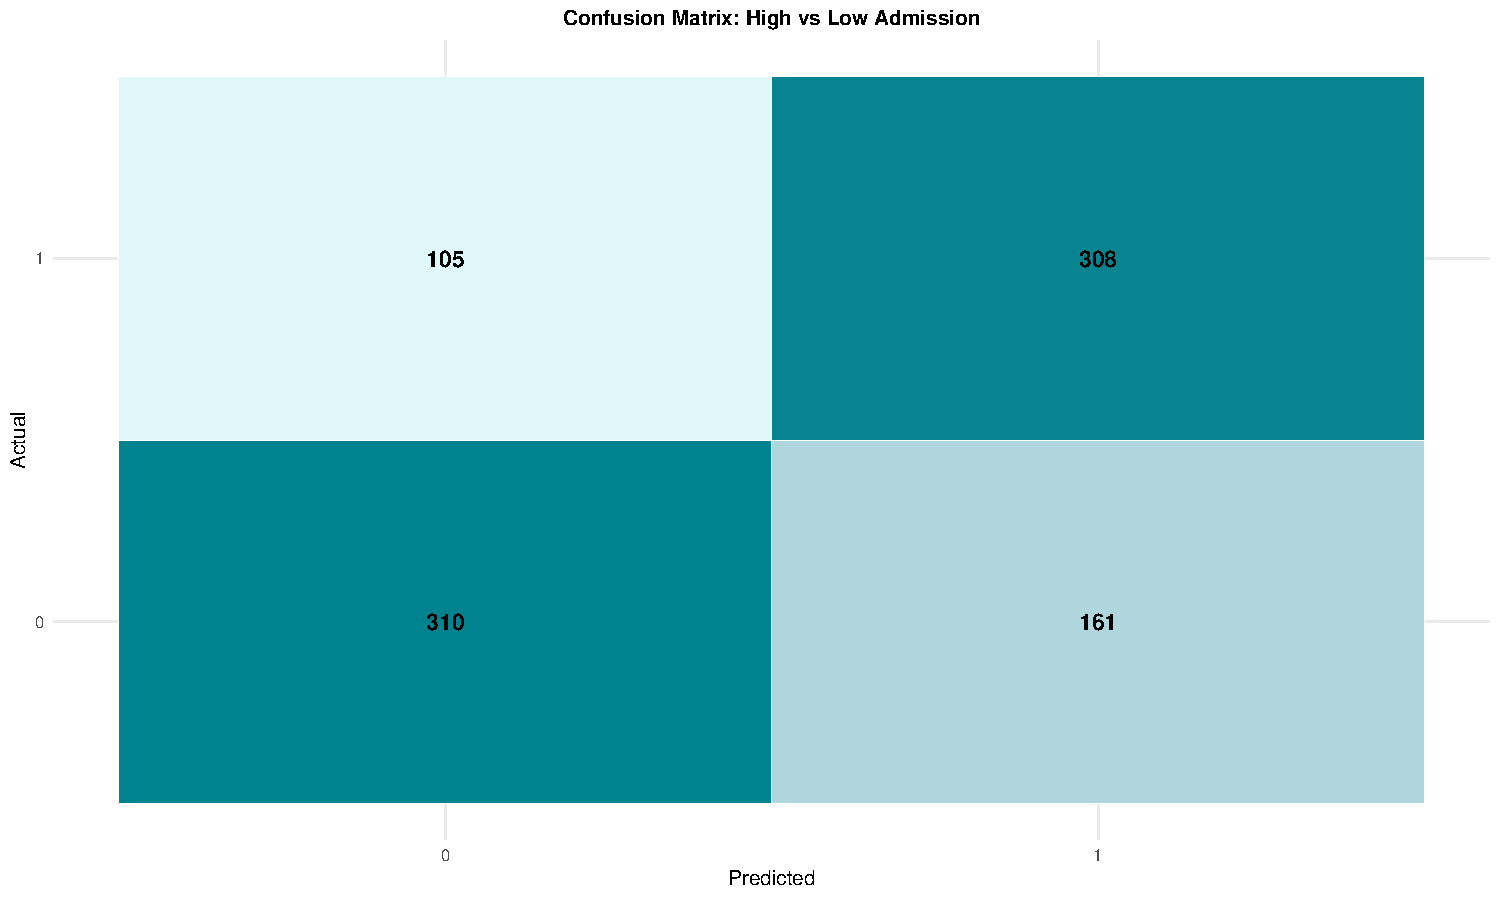
\includegraphics{final_report_ml1_group_files/figure-latex/binomial1-eval-1} \end{center}

On the test set, the admission model achieves \textbf{accuracy = 0.699}
(\textasciitilde70\% correct classifications). This is better than
random guessing but leaves room for improvement; it correctly flags most
high/low admission cases, but about 3 in 10 are still misclassified.

\subsubsection{ROC Curve Analysis}\label{roc-curve-analysis}

\begin{Shaded}
\begin{Highlighting}[]
\NormalTok{roc\_adm }\OtherTok{\textless{}{-}} \FunctionTok{roc}\NormalTok{(test\_adm\_scaled}\SpecialCharTok{$}\NormalTok{High\_Admission, pred\_adm\_prob, }\AttributeTok{quiet =} \ConstantTok{TRUE}\NormalTok{)}
\NormalTok{auc\_adm }\OtherTok{\textless{}{-}} \FunctionTok{auc}\NormalTok{(roc\_adm)}

\FunctionTok{plot}\NormalTok{(roc\_adm, }\AttributeTok{col =} \StringTok{"darkorange"}\NormalTok{, }\AttributeTok{lwd =} \DecValTok{2}\NormalTok{,}
     \AttributeTok{main =} \FunctionTok{sprintf}\NormalTok{(}\StringTok{"ROC Curve {-} High Admission (AUC = \%.3f)"}\NormalTok{, auc\_adm))}
\FunctionTok{abline}\NormalTok{(}\AttributeTok{a =} \DecValTok{0}\NormalTok{, }\AttributeTok{b =} \DecValTok{1}\NormalTok{, }\AttributeTok{lty =} \DecValTok{2}\NormalTok{, }\AttributeTok{col =} \StringTok{"navy"}\NormalTok{, }\AttributeTok{lwd =} \DecValTok{2}\NormalTok{)}
\FunctionTok{grid}\NormalTok{()}
\end{Highlighting}
\end{Shaded}

\begin{figure}

{\centering 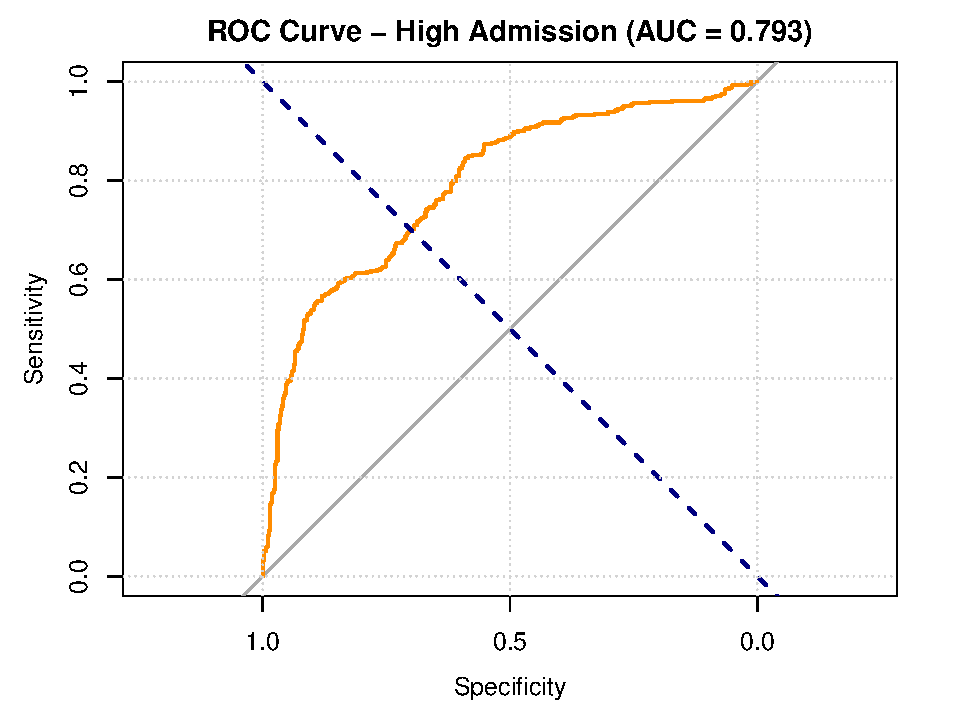
\includegraphics{final_report_ml1_group_files/figure-latex/binomial1-roc-1} 

}

\caption{ROC Curve - High Admission}\label{fig:binomial1-roc}
\end{figure}

\textbf{Understanding the ROC Curve:} The \textbf{AUC} of 0.793
quantifies overall discrimination ability. \textbf{AUC \textgreater{}
0.7} indicates acceptable discrimination, while \textbf{AUC
\textgreater{} 0.8} represents excellent performance.

\subsubsection{Interpreting Odds Ratios}\label{interpreting-odds-ratios}

\begin{Shaded}
\begin{Highlighting}[]
\NormalTok{coef\_df\_adm }\OtherTok{\textless{}{-}} \FunctionTok{data.frame}\NormalTok{(}
  \AttributeTok{Feature =}\NormalTok{ features\_admission,}
  \AttributeTok{Coefficient =} \FunctionTok{coef}\NormalTok{(glm\_adm)[}\SpecialCharTok{{-}}\DecValTok{1}\NormalTok{],}
  \AttributeTok{Odds\_Ratio =} \FunctionTok{exp}\NormalTok{(}\FunctionTok{coef}\NormalTok{(glm\_adm)[}\SpecialCharTok{{-}}\DecValTok{1}\NormalTok{])}
\NormalTok{) }\SpecialCharTok{\%\textgreater{}\%}
  \FunctionTok{arrange}\NormalTok{(}\FunctionTok{desc}\NormalTok{(}\FunctionTok{abs}\NormalTok{(Coefficient)))}

\NormalTok{odds\_table\_adm }\OtherTok{\textless{}{-}}\NormalTok{ coef\_df\_adm }\SpecialCharTok{\%\textgreater{}\%}
  \FunctionTok{mutate}\NormalTok{(}\AttributeTok{Abs\_Coefficient =} \FunctionTok{abs}\NormalTok{(Coefficient)) }\SpecialCharTok{\%\textgreater{}\%}
  \FunctionTok{arrange}\NormalTok{(}\FunctionTok{desc}\NormalTok{(Abs\_Coefficient)) }\SpecialCharTok{\%\textgreater{}\%}
  \FunctionTok{select}\NormalTok{(Feature, Coefficient, Odds\_Ratio) }\SpecialCharTok{\%\textgreater{}\%}
  \FunctionTok{head}\NormalTok{(}\DecValTok{10}\NormalTok{)}

\NormalTok{knitr}\SpecialCharTok{::}\FunctionTok{kable}\NormalTok{(odds\_table\_adm, }\AttributeTok{caption =} \StringTok{"Top 10 admission predictors (log{-}odds and odds ratio)"}\NormalTok{)}
\end{Highlighting}
\end{Shaded}

\begin{longtable}[]{@{}
  >{\raggedright\arraybackslash}p{(\linewidth - 6\tabcolsep) * \real{0.3647}}
  >{\raggedright\arraybackslash}p{(\linewidth - 6\tabcolsep) * \real{0.3647}}
  >{\raggedleft\arraybackslash}p{(\linewidth - 6\tabcolsep) * \real{0.1412}}
  >{\raggedleft\arraybackslash}p{(\linewidth - 6\tabcolsep) * \real{0.1294}}@{}}
\caption{Top 10 admission predictors (log-odds and odds
ratio)}\tabularnewline
\toprule\noalign{}
\begin{minipage}[b]{\linewidth}\raggedright
\end{minipage} & \begin{minipage}[b]{\linewidth}\raggedright
Feature
\end{minipage} & \begin{minipage}[b]{\linewidth}\raggedleft
Coefficient
\end{minipage} & \begin{minipage}[b]{\linewidth}\raggedleft
Odds\_Ratio
\end{minipage} \\
\midrule\noalign{}
\endfirsthead
\toprule\noalign{}
\begin{minipage}[b]{\linewidth}\raggedright
\end{minipage} & \begin{minipage}[b]{\linewidth}\raggedright
Feature
\end{minipage} & \begin{minipage}[b]{\linewidth}\raggedleft
Coefficient
\end{minipage} & \begin{minipage}[b]{\linewidth}\raggedleft
Odds\_Ratio
\end{minipage} \\
\midrule\noalign{}
\endhead
\bottomrule\noalign{}
\endlastfoot
Previous.qualification..grade. & Previous.qualification..grade. &
1.4992155 & 4.4781746 \\
Application.order & Application.order & -0.1564085 & 0.8552098 \\
Displaced & Displaced & 0.1434473 & 1.1542460 \\
Father.s.qualification & Father.s.qualification & -0.0799645 &
0.9231492 \\
Age.at.enrollment & Age.at.enrollment & 0.0607805 & 1.0626657 \\
Gender & Gender & 0.0367061 & 1.0373880 \\
International & International & 0.0352621 & 1.0358912 \\
Mother.s.qualification & Mother.s.qualification & 0.0168197 &
1.0169619 \\
Scholarship.holder & Scholarship.holder & -0.0130452 & 0.9870395 \\
\end{longtable}

\subsection{5.3 Model 2: Predicting Graduation vs
Dropout}\label{model-2-predicting-graduation-vs-dropout}

\textbf{This is our most actionable model}---identifying students
\textbf{at risk of dropping out} enables \textbf{targeted
interventions}.

\subsubsection{5.3 Binomial GLM: Graduation vs
Dropout}\label{binomial-glm-graduation-vs-dropout}

Graduation dataset \textbar{} Dropout=1421 \textbar{} Graduate=2209
Binomial (Graduation) dataset: 3630 students Binomial GLM (Graduation)
accuracy: 0.8416 (84.16\%) Binomial GLM (Graduation) AUC: 0.888

Top 5 Predictors Interpretation: ✓ Curricular.units.1st.sem..approved.:
359.5\% increase in graduation odds per SD increase ✓
Tuition.fees.up.to.date: 157.8\% increase in graduation odds per SD
increase ✓ Scholarship.holder: 74.1\% increase in graduation odds per SD
increase ✗ Age.at.enrollment: 34.5\% decrease in graduation odds per SD
increase ✗ Debtor: 30.0\% decrease in graduation odds per SD increase

\begin{longtable}[]{@{}
  >{\raggedright\arraybackslash}p{(\linewidth - 6\tabcolsep) * \real{0.3789}}
  >{\raggedright\arraybackslash}p{(\linewidth - 6\tabcolsep) * \real{0.3789}}
  >{\raggedleft\arraybackslash}p{(\linewidth - 6\tabcolsep) * \real{0.1263}}
  >{\raggedleft\arraybackslash}p{(\linewidth - 6\tabcolsep) * \real{0.1158}}@{}}
\caption{Top 3 graduation predictors (log-odds and odds
ratio)}\tabularnewline
\toprule\noalign{}
\begin{minipage}[b]{\linewidth}\raggedright
\end{minipage} & \begin{minipage}[b]{\linewidth}\raggedright
Feature
\end{minipage} & \begin{minipage}[b]{\linewidth}\raggedleft
Coefficient
\end{minipage} & \begin{minipage}[b]{\linewidth}\raggedleft
Odds\_Ratio
\end{minipage} \\
\midrule\noalign{}
\endfirsthead
\toprule\noalign{}
\begin{minipage}[b]{\linewidth}\raggedright
\end{minipage} & \begin{minipage}[b]{\linewidth}\raggedright
Feature
\end{minipage} & \begin{minipage}[b]{\linewidth}\raggedleft
Coefficient
\end{minipage} & \begin{minipage}[b]{\linewidth}\raggedleft
Odds\_Ratio
\end{minipage} \\
\midrule\noalign{}
\endhead
\bottomrule\noalign{}
\endlastfoot
Curricular.units.1st.sem..approved. &
Curricular.units.1st.sem..approved. & 1.5250141 & 4.595208 \\
Tuition.fees.up.to.date & Tuition.fees.up.to.date & 0.9471399 &
2.578325 \\
Scholarship.holder & Scholarship.holder & 0.5543312 & 1.740776 \\
\end{longtable}

We model graduation vs dropout in one step: build the binary target,
split/scale, train a binomial GLM, and summarize discrimination (AUC)
plus odds ratios for the most influential features. The model delivers
\textbf{AUC = 0.888}, showing strong abilit to predict graduates and
dropouts. First-semester performance and financial factors are proven to
be top factors.

\textbf{Actionable Insights:} \textbf{First semester performance}
emerges as the dominant predictor. \textbf{Financial factors} (debtor
status, tuition payment) also show strong effects, suggesting that
financial aid could meaningfully impact retention.

\begin{center}\rule{0.5\linewidth}{0.5pt}\end{center}

\section{6. Generalized Linear Model -
Poisson}\label{generalized-linear-model---poisson}

\subsection{6.1 Why Poisson Regression?}\label{why-poisson-regression}

Course completion counts represent non-negative integers (0, 1, 2,
3\ldots) that don't follow a normal distribution. Poisson regression
solves this by:

\begin{enumerate}
\def\labelenumi{\arabic{enumi}.}
\tightlist
\item
  \textbf{Ensuring non-negative predictions} through a log link function
\item
  \textbf{Modeling the count distribution} appropriately
\item
  \textbf{Accounting for variance} that changes with the mean
\end{enumerate}

The model structure is:
\(\log(\lambda) = \beta_0 + \beta_1X_1 + ... + \beta_nX_n\), where
\(\lambda\) represents the expected count.

\subsection{6.2 Model 1: First Semester Course
Approvals}\label{model-1-first-semester-course-approvals}

Understanding what predicts first semester success is crucial for early
intervention.

\subsubsection{Data Preparation}\label{data-preparation-1}

\begin{Shaded}
\begin{Highlighting}[]
\NormalTok{TARGET\_1 }\OtherTok{\textless{}{-}} \StringTok{\textquotesingle{}Curricular.units.1st.sem..approved.\textquotesingle{}}

\NormalTok{FEATURES\_1 }\OtherTok{\textless{}{-}} \FunctionTok{c}\NormalTok{(}
    \StringTok{\textquotesingle{}Previous.qualification..grade.\textquotesingle{}}\NormalTok{,}
    \StringTok{\textquotesingle{}Admission.grade\textquotesingle{}}\NormalTok{,}
    \StringTok{\textquotesingle{}Age.at.enrollment\textquotesingle{}}\NormalTok{,}
    \StringTok{"Mother.s.qualification"}\NormalTok{,}
    \StringTok{"Father.s.qualification"}\NormalTok{,}
    \StringTok{\textquotesingle{}Scholarship.holder\textquotesingle{}}\NormalTok{,}
    \StringTok{\textquotesingle{}Gender\textquotesingle{}}\NormalTok{,}
    \StringTok{\textquotesingle{}Debtor\textquotesingle{}}\NormalTok{,}
    \StringTok{\textquotesingle{}Tuition.fees.up.to.date\textquotesingle{}}\NormalTok{,}
    \StringTok{\textquotesingle{}Curricular.units.1st.sem..enrolled.\textquotesingle{}}\NormalTok{,}
    \StringTok{\textquotesingle{}Unemployment.rate\textquotesingle{}}\NormalTok{,}
    \StringTok{\textquotesingle{}GDP\textquotesingle{}}
\NormalTok{)}

\NormalTok{df\_model1 }\OtherTok{\textless{}{-}}\NormalTok{ df }\SpecialCharTok{\%\textgreater{}\%}
    \FunctionTok{select}\NormalTok{(}\FunctionTok{all\_of}\NormalTok{(}\FunctionTok{c}\NormalTok{(FEATURES\_1, TARGET\_1))) }\SpecialCharTok{\%\textgreater{}\%}
    \FunctionTok{mutate}\NormalTok{(}\FunctionTok{across}\NormalTok{(}\FunctionTok{everything}\NormalTok{(), }\SpecialCharTok{\textasciitilde{}} \FunctionTok{as.numeric}\NormalTok{(}\FunctionTok{as.character}\NormalTok{(.)))) }\SpecialCharTok{\%\textgreater{}\%}
    \FunctionTok{drop\_na}\NormalTok{()}

\FunctionTok{cat}\NormalTok{(}\FunctionTok{sprintf}\NormalTok{(}\StringTok{"Poisson dataset (1st semester approvals): \%d students}\SpecialCharTok{\textbackslash{}n}\StringTok{"}\NormalTok{, }\FunctionTok{nrow}\NormalTok{(df\_model1)))}
\FunctionTok{set.seed}\NormalTok{(}\DecValTok{42}\NormalTok{)}
\NormalTok{X1 }\OtherTok{\textless{}{-}}\NormalTok{ df\_model1 }\SpecialCharTok{\%\textgreater{}\%}\NormalTok{ dplyr}\SpecialCharTok{::}\FunctionTok{select}\NormalTok{(}\FunctionTok{all\_of}\NormalTok{(FEATURES\_1))}
\NormalTok{y1 }\OtherTok{\textless{}{-}}\NormalTok{ df\_model1[[TARGET\_1]]}

\NormalTok{train\_idx1 }\OtherTok{\textless{}{-}} \FunctionTok{createDataPartition}\NormalTok{(y1, }\AttributeTok{p =} \FloatTok{0.8}\NormalTok{, }\AttributeTok{list =} \ConstantTok{FALSE}\NormalTok{)}
\NormalTok{X\_train1 }\OtherTok{\textless{}{-}}\NormalTok{ X1[train\_idx1, ]}
\NormalTok{X\_test1  }\OtherTok{\textless{}{-}}\NormalTok{ X1[}\SpecialCharTok{{-}}\NormalTok{train\_idx1, ]}
\NormalTok{y\_train1 }\OtherTok{\textless{}{-}}\NormalTok{ y1[train\_idx1]}
\NormalTok{y\_test1  }\OtherTok{\textless{}{-}}\NormalTok{ y1[}\SpecialCharTok{{-}}\NormalTok{train\_idx1]}

\NormalTok{train\_data1 }\OtherTok{\textless{}{-}}\NormalTok{ X\_train1}
\NormalTok{train\_data1[[TARGET\_1]] }\OtherTok{\textless{}{-}}\NormalTok{ y\_train1}

\NormalTok{poisson\_model1 }\OtherTok{\textless{}{-}} \FunctionTok{glm}\NormalTok{(}
  \AttributeTok{formula =} \FunctionTok{as.formula}\NormalTok{(}\FunctionTok{paste}\NormalTok{(TARGET\_1, }\StringTok{"\textasciitilde{} ."}\NormalTok{)),}
  \AttributeTok{family =} \FunctionTok{poisson}\NormalTok{(}\AttributeTok{link =} \StringTok{"log"}\NormalTok{),}
  \AttributeTok{data =}\NormalTok{ train\_data1}
\NormalTok{)}

\CommentTok{\# {-}{-}{-} Performance}
\NormalTok{y\_pred\_train1 }\OtherTok{\textless{}{-}} \FunctionTok{predict}\NormalTok{(poisson\_model1, }\AttributeTok{newdata =}\NormalTok{ X\_train1, }\AttributeTok{type =} \StringTok{"response"}\NormalTok{)}
\NormalTok{y\_pred\_test1 }\OtherTok{\textless{}{-}} \FunctionTok{predict}\NormalTok{(poisson\_model1, }\AttributeTok{newdata =}\NormalTok{ X\_test1, }\AttributeTok{type =} \StringTok{"response"}\NormalTok{)}

\NormalTok{train\_rmse1 }\OtherTok{\textless{}{-}} \FunctionTok{sqrt}\NormalTok{(}\FunctionTok{mean}\NormalTok{((y\_train1 }\SpecialCharTok{{-}}\NormalTok{ y\_pred\_train1)}\SpecialCharTok{\^{}}\DecValTok{2}\NormalTok{))}
\NormalTok{train\_mae1 }\OtherTok{\textless{}{-}} \FunctionTok{mean}\NormalTok{(}\FunctionTok{abs}\NormalTok{(y\_train1 }\SpecialCharTok{{-}}\NormalTok{ y\_pred\_train1))}

\NormalTok{test\_rmse1 }\OtherTok{\textless{}{-}} \FunctionTok{sqrt}\NormalTok{(}\FunctionTok{mean}\NormalTok{((y\_test1 }\SpecialCharTok{{-}}\NormalTok{ y\_pred\_test1)}\SpecialCharTok{\^{}}\DecValTok{2}\NormalTok{))}
\NormalTok{test\_mae1 }\OtherTok{\textless{}{-}} \FunctionTok{mean}\NormalTok{(}\FunctionTok{abs}\NormalTok{(y\_test1 }\SpecialCharTok{{-}}\NormalTok{ y\_pred\_test1))}
\NormalTok{test\_r2\_1 }\OtherTok{\textless{}{-}} \FunctionTok{cor}\NormalTok{(y\_test1, y\_pred\_test1)}\SpecialCharTok{\^{}}\DecValTok{2}

\FunctionTok{cat}\NormalTok{(}\FunctionTok{sprintf}\NormalTok{(}\StringTok{"Poisson GLM performance | Train RMSE=\%.4f MAE=\%.4f | Test RMSE=\%.4f MAE=\%.4f R²=\%.4f}\SpecialCharTok{\textbackslash{}n}\StringTok{"}\NormalTok{,}
\NormalTok{            train\_rmse1, train\_mae1, test\_rmse1, test\_mae1, test\_r2\_1))}

\CommentTok{\# {-}{-}{-} Rate ratios (top 3)}
\NormalTok{coef\_summary1 }\OtherTok{\textless{}{-}} \FunctionTok{summary}\NormalTok{(poisson\_model1)}\SpecialCharTok{$}\NormalTok{coefficients}
\NormalTok{coef\_df1 }\OtherTok{\textless{}{-}} \FunctionTok{data.frame}\NormalTok{(}
    \AttributeTok{Feature =} \FunctionTok{rownames}\NormalTok{(coef\_summary1),}
    \AttributeTok{Coefficient =}\NormalTok{ coef\_summary1[, }\StringTok{"Estimate"}\NormalTok{],}
    \AttributeTok{Rate\_Ratio =} \FunctionTok{exp}\NormalTok{(coef\_summary1[, }\StringTok{"Estimate"}\NormalTok{]),}
    \AttributeTok{P\_value =}\NormalTok{ coef\_summary1[, }\StringTok{"Pr(\textgreater{}|z|)"}\NormalTok{]}
\NormalTok{) }\SpecialCharTok{\%\textgreater{}\%}
    \FunctionTok{mutate}\NormalTok{(}\AttributeTok{Abs\_Coef =} \FunctionTok{abs}\NormalTok{(Coefficient)) }\SpecialCharTok{\%\textgreater{}\%}
    \FunctionTok{arrange}\NormalTok{(}\FunctionTok{desc}\NormalTok{(Abs\_Coef))}

\NormalTok{top\_poisson\_tbl }\OtherTok{\textless{}{-}}\NormalTok{ coef\_df1[, }\FunctionTok{c}\NormalTok{(}\StringTok{"Feature"}\NormalTok{, }\StringTok{"Coefficient"}\NormalTok{, }\StringTok{"Rate\_Ratio"}\NormalTok{, }\StringTok{"P\_value"}\NormalTok{)] }\SpecialCharTok{\%\textgreater{}\%}
  \FunctionTok{head}\NormalTok{(}\DecValTok{3}\NormalTok{)}

\NormalTok{knitr}\SpecialCharTok{::}\FunctionTok{kable}\NormalTok{(top\_poisson\_tbl, }\AttributeTok{caption =} \StringTok{"Top 3 Poisson GLM predictors (coefficient and rate ratio)"}\NormalTok{)}

\CommentTok{\# {-}{-}{-} Coefficient bar plot (inline, compact)}
\NormalTok{coef\_plot\_df }\OtherTok{\textless{}{-}}\NormalTok{ coef\_df1 }\SpecialCharTok{\%\textgreater{}\%}
    \FunctionTok{filter}\NormalTok{(Feature }\SpecialCharTok{!=} \StringTok{"(Intercept)"}\NormalTok{) }\SpecialCharTok{\%\textgreater{}\%}
    \FunctionTok{head}\NormalTok{(}\DecValTok{10}\NormalTok{)}

\FunctionTok{par}\NormalTok{(}\AttributeTok{mar =} \FunctionTok{c}\NormalTok{(}\DecValTok{5}\NormalTok{, }\DecValTok{10}\NormalTok{, }\DecValTok{3}\NormalTok{, }\DecValTok{2}\NormalTok{), }\AttributeTok{cex =} \FloatTok{0.8}\NormalTok{)}
\NormalTok{colors }\OtherTok{\textless{}{-}} \FunctionTok{ifelse}\NormalTok{(coef\_plot\_df}\SpecialCharTok{$}\NormalTok{Coefficient }\SpecialCharTok{\textgreater{}} \DecValTok{0}\NormalTok{, }\StringTok{"green"}\NormalTok{, }\StringTok{"red"}\NormalTok{)}
\FunctionTok{barplot}\NormalTok{(coef\_plot\_df}\SpecialCharTok{$}\NormalTok{Coefficient,}
        \AttributeTok{names.arg =}\NormalTok{ coef\_plot\_df}\SpecialCharTok{$}\NormalTok{Feature,}
        \AttributeTok{horiz =} \ConstantTok{TRUE}\NormalTok{,}
        \AttributeTok{las =} \DecValTok{1}\NormalTok{,}
        \AttributeTok{col =} \FunctionTok{adjustcolor}\NormalTok{(colors, }\AttributeTok{alpha.f =} \FloatTok{0.7}\NormalTok{),}
        \AttributeTok{xlab =} \StringTok{"Coefficient (Log Rate)"}\NormalTok{,}
        \AttributeTok{main =} \StringTok{"Feature Effects on Course Approvals"}\NormalTok{)}
\FunctionTok{abline}\NormalTok{(}\AttributeTok{v =} \DecValTok{0}\NormalTok{, }\AttributeTok{col =} \StringTok{"black"}\NormalTok{, }\AttributeTok{lwd =} \DecValTok{1}\NormalTok{)}
\FunctionTok{grid}\NormalTok{()}
\end{Highlighting}
\end{Shaded}

\begin{center}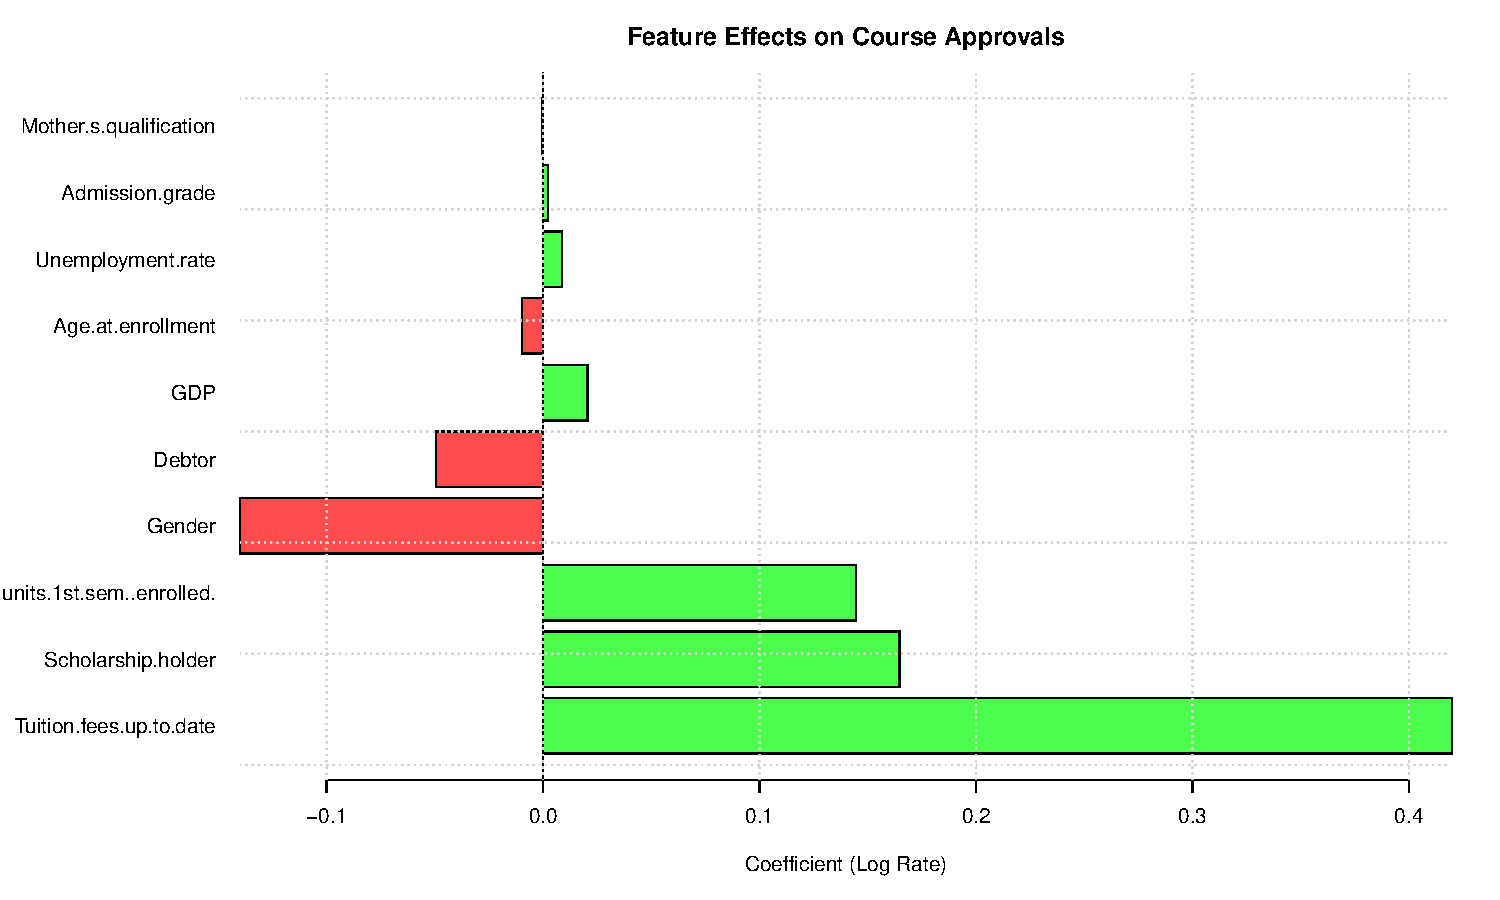
\includegraphics{final_report_ml1_group_files/figure-latex/poisson1-prep-1} \end{center}

\begin{Shaded}
\begin{Highlighting}[]
\CommentTok{\# Store for plots below}
\FunctionTok{assign}\NormalTok{(}\StringTok{"coef\_df1"}\NormalTok{, coef\_df1, }\AttributeTok{envir =}\NormalTok{ .GlobalEnv)}
\FunctionTok{assign}\NormalTok{(}\StringTok{"y\_pred\_train1"}\NormalTok{, y\_pred\_train1, }\AttributeTok{envir =}\NormalTok{ .GlobalEnv)}
\FunctionTok{assign}\NormalTok{(}\StringTok{"y\_pred\_test1"}\NormalTok{, y\_pred\_test1, }\AttributeTok{envir =}\NormalTok{ .GlobalEnv)}
\FunctionTok{assign}\NormalTok{(}\StringTok{"y\_train1"}\NormalTok{, y\_train1, }\AttributeTok{envir =}\NormalTok{ .GlobalEnv)}
\FunctionTok{assign}\NormalTok{(}\StringTok{"y\_test1"}\NormalTok{, y\_test1, }\AttributeTok{envir =}\NormalTok{ .GlobalEnv)}
\end{Highlighting}
\end{Shaded}

\textbf{Interpreting Rate Ratios:} Rate ratios show how the expected
course count changes per unit increase. For example, a rate ratio of
\textbf{1.30} means \textbf{30\% more courses} on average; \textbf{0.80}
means \textbf{20\% fewer}.

\subsubsection{Visualization of RMSE}\label{visualization-of-rmse}

\begin{Shaded}
\begin{Highlighting}[]
\FunctionTok{par}\NormalTok{(}\AttributeTok{mfrow =} \FunctionTok{c}\NormalTok{(}\DecValTok{1}\NormalTok{, }\DecValTok{2}\NormalTok{))}

\FunctionTok{plot}\NormalTok{(y\_train1, y\_pred\_train1,}
     \AttributeTok{xlab =} \StringTok{"Actual Courses"}\NormalTok{, }\AttributeTok{ylab =} \StringTok{"Predicted Courses"}\NormalTok{,}
     \AttributeTok{main =} \FunctionTok{sprintf}\NormalTok{(}\StringTok{"Training (RMSE = \%.3f)"}\NormalTok{,}
                    \FunctionTok{sqrt}\NormalTok{(}\FunctionTok{mean}\NormalTok{((y\_train1 }\SpecialCharTok{{-}}\NormalTok{ y\_pred\_train1)}\SpecialCharTok{\^{}}\DecValTok{2}\NormalTok{))),}
     \AttributeTok{pch =} \DecValTok{16}\NormalTok{, }\AttributeTok{col =} \FunctionTok{rgb}\NormalTok{(}\DecValTok{0}\NormalTok{, }\DecValTok{0}\NormalTok{, }\DecValTok{1}\NormalTok{, }\FloatTok{0.5}\NormalTok{))}
\FunctionTok{abline}\NormalTok{(}\AttributeTok{a =} \DecValTok{0}\NormalTok{, }\AttributeTok{b =} \DecValTok{1}\NormalTok{, }\AttributeTok{col =} \StringTok{"red"}\NormalTok{, }\AttributeTok{lwd =} \DecValTok{2}\NormalTok{, }\AttributeTok{lty =} \DecValTok{2}\NormalTok{)}
\FunctionTok{grid}\NormalTok{()}

\FunctionTok{plot}\NormalTok{(y\_test1, y\_pred\_test1,}
     \AttributeTok{xlab =} \StringTok{"Actual Courses"}\NormalTok{, }\AttributeTok{ylab =} \StringTok{"Predicted Courses"}\NormalTok{,}
     \AttributeTok{main =} \FunctionTok{sprintf}\NormalTok{(}\StringTok{"Test (RMSE = \%.3f)"}\NormalTok{, test\_rmse1),}
     \AttributeTok{pch =} \DecValTok{16}\NormalTok{, }\AttributeTok{col =} \FunctionTok{rgb}\NormalTok{(}\DecValTok{0}\NormalTok{, }\DecValTok{1}\NormalTok{, }\DecValTok{0}\NormalTok{, }\FloatTok{0.5}\NormalTok{))}
\FunctionTok{abline}\NormalTok{(}\AttributeTok{a =} \DecValTok{0}\NormalTok{, }\AttributeTok{b =} \DecValTok{1}\NormalTok{, }\AttributeTok{col =} \StringTok{"red"}\NormalTok{, }\AttributeTok{lwd =} \DecValTok{2}\NormalTok{, }\AttributeTok{lty =} \DecValTok{2}\NormalTok{)}
\FunctionTok{grid}\NormalTok{()}
\end{Highlighting}
\end{Shaded}

\begin{figure}

{\centering 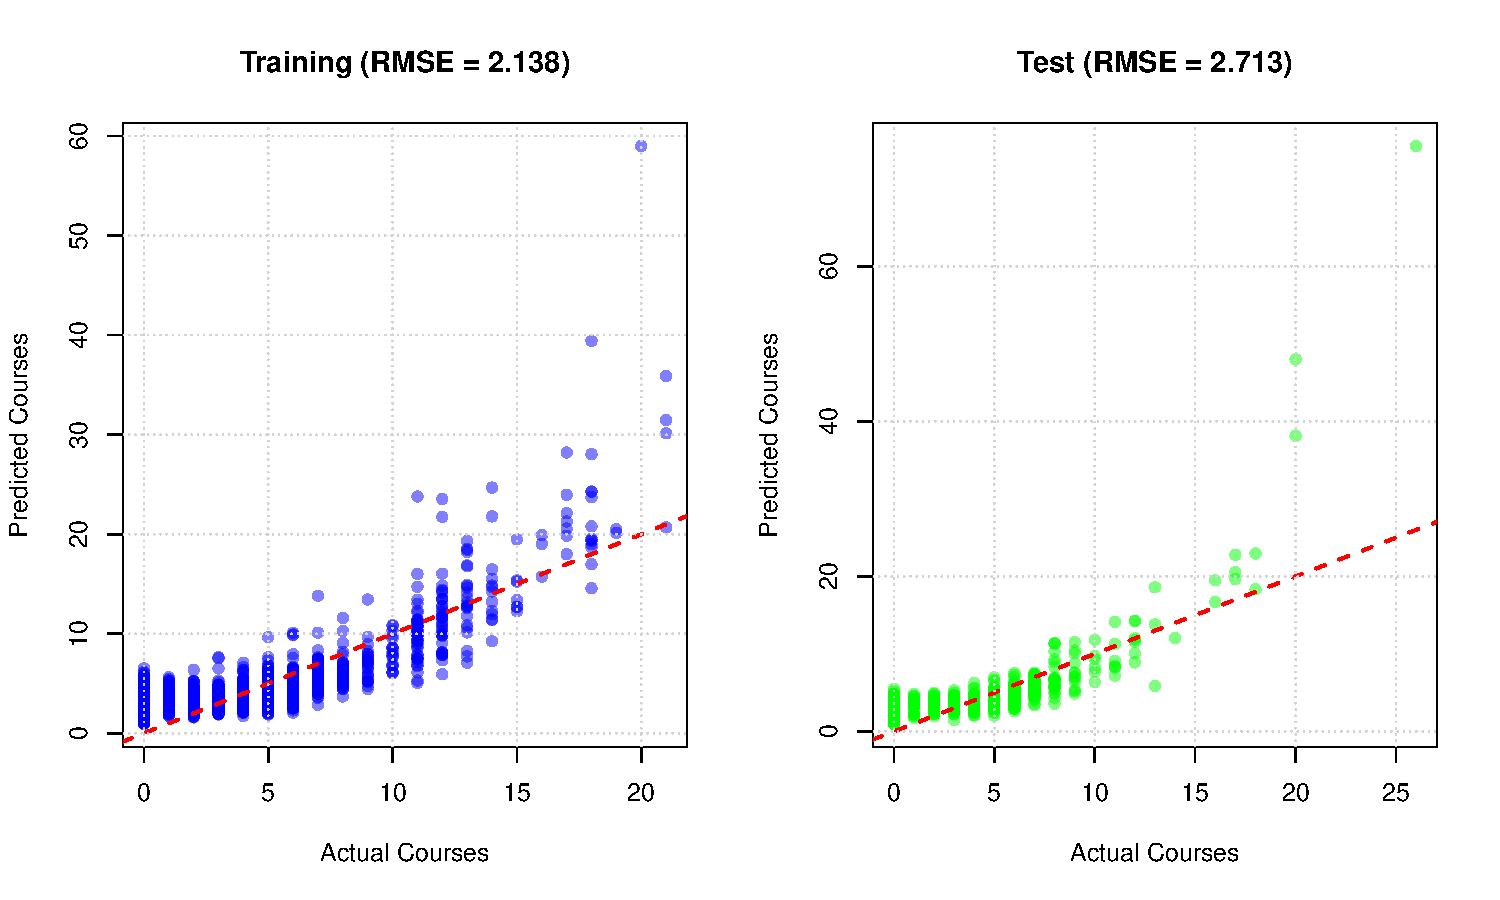
\includegraphics{final_report_ml1_group_files/figure-latex/poisson1-plots-1} 

}

\caption{Model predictions for course approvals}\label{fig:poisson1-plots}
\end{figure}

\textbf{RMSE reminder:} is the square-root of the average squared error;
lower values mean predictions stay closer to actual course counts. Here
the test RMSE shows the typical error distance (in courses) between
predicted and actual approvals. The plots show a reasonable fit for
common counts, but the model tends to underpredict for very high course
approvals, so extreme tails are harder to capture.

\subsection{6.3 Model 2: Second Semester Course
Approvals}\label{model-2-second-semester-course-approvals}

\begin{Shaded}
\begin{Highlighting}[]
\NormalTok{TARGET\_2 }\OtherTok{\textless{}{-}} \StringTok{\textquotesingle{}Curricular.units.2nd.sem..approved.\textquotesingle{}}

\NormalTok{FEATURES\_2 }\OtherTok{\textless{}{-}} \FunctionTok{c}\NormalTok{(}
    \StringTok{\textquotesingle{}Previous.qualification..grade.\textquotesingle{}}\NormalTok{,}
    \StringTok{\textquotesingle{}Admission.grade\textquotesingle{}}\NormalTok{,}
    \StringTok{\textquotesingle{}Age.at.enrollment\textquotesingle{}}\NormalTok{,}
    \StringTok{\textquotesingle{}Scholarship.holder\textquotesingle{}}\NormalTok{,}
    \StringTok{\textquotesingle{}Debtor\textquotesingle{}}\NormalTok{,}
    \StringTok{\textquotesingle{}Tuition.fees.up.to.date\textquotesingle{}}\NormalTok{,}
    \StringTok{\textquotesingle{}Curricular.units.1st.sem..approved.\textquotesingle{}}\NormalTok{,}
    \StringTok{\textquotesingle{}Curricular.units.1st.sem..grade.\textquotesingle{}}\NormalTok{,}
    \StringTok{\textquotesingle{}Curricular.units.2nd.sem..enrolled.\textquotesingle{}}\NormalTok{,}
    \StringTok{\textquotesingle{}Unemployment.rate\textquotesingle{}}\NormalTok{,}
    \StringTok{\textquotesingle{}GDP\textquotesingle{}}
\NormalTok{)}

\NormalTok{df\_model2 }\OtherTok{\textless{}{-}}\NormalTok{ df }\SpecialCharTok{\%\textgreater{}\%}
    \FunctionTok{select}\NormalTok{(}\FunctionTok{all\_of}\NormalTok{(}\FunctionTok{c}\NormalTok{(FEATURES\_2, TARGET\_2))) }\SpecialCharTok{\%\textgreater{}\%}
    \FunctionTok{mutate}\NormalTok{(}\FunctionTok{across}\NormalTok{(}\FunctionTok{everything}\NormalTok{(), }\SpecialCharTok{\textasciitilde{}} \FunctionTok{as.numeric}\NormalTok{(}\FunctionTok{as.character}\NormalTok{(.)))) }\SpecialCharTok{\%\textgreater{}\%}
    \FunctionTok{drop\_na}\NormalTok{()}

\FunctionTok{cat}\NormalTok{(}\FunctionTok{sprintf}\NormalTok{(}\StringTok{"Poisson dataset (2nd semester approvals): \%d students}\SpecialCharTok{\textbackslash{}n}\StringTok{"}\NormalTok{, }\FunctionTok{nrow}\NormalTok{(df\_model2)))}
\end{Highlighting}
\end{Shaded}

For second semester approvals (count of courses passed), we again use a
Poisson model on \textbf{4424} students.

\begin{Shaded}
\begin{Highlighting}[]
\FunctionTok{set.seed}\NormalTok{(}\DecValTok{42}\NormalTok{)}

\NormalTok{X2 }\OtherTok{\textless{}{-}}\NormalTok{ df\_model2 }\SpecialCharTok{\%\textgreater{}\%} \FunctionTok{select}\NormalTok{(}\FunctionTok{all\_of}\NormalTok{(FEATURES\_2))}
\NormalTok{y2 }\OtherTok{\textless{}{-}}\NormalTok{ df\_model2[[TARGET\_2]]}

\NormalTok{trainIndex2 }\OtherTok{\textless{}{-}} \FunctionTok{createDataPartition}\NormalTok{(y2, }\AttributeTok{p =} \FloatTok{0.8}\NormalTok{, }\AttributeTok{list =} \ConstantTok{FALSE}\NormalTok{)}

\NormalTok{X\_train2 }\OtherTok{\textless{}{-}}\NormalTok{ X2[trainIndex2, ]}
\NormalTok{X\_test2 }\OtherTok{\textless{}{-}}\NormalTok{ X2[}\SpecialCharTok{{-}}\NormalTok{trainIndex2, ]}
\NormalTok{y\_train2 }\OtherTok{\textless{}{-}}\NormalTok{ y2[trainIndex2]}
\NormalTok{y\_test2 }\OtherTok{\textless{}{-}}\NormalTok{ y2[}\SpecialCharTok{{-}}\NormalTok{trainIndex2]}

\NormalTok{train\_data2 }\OtherTok{\textless{}{-}}\NormalTok{ X\_train2}
\NormalTok{train\_data2[[TARGET\_2]] }\OtherTok{\textless{}{-}}\NormalTok{ y\_train2}

\NormalTok{formula\_2 }\OtherTok{\textless{}{-}} \FunctionTok{as.formula}\NormalTok{(}\FunctionTok{paste}\NormalTok{(TARGET\_2, }\StringTok{"\textasciitilde{}"}\NormalTok{, }\FunctionTok{paste}\NormalTok{(FEATURES\_2, }\AttributeTok{collapse =} \StringTok{" + "}\NormalTok{)))}

\NormalTok{poisson\_model2 }\OtherTok{\textless{}{-}} \FunctionTok{glm}\NormalTok{(formula\_2, }\AttributeTok{data =}\NormalTok{ train\_data2, }\AttributeTok{family =} \FunctionTok{poisson}\NormalTok{(}\AttributeTok{link =} \StringTok{"log"}\NormalTok{))}
\end{Highlighting}
\end{Shaded}

\begin{Shaded}
\begin{Highlighting}[]
\NormalTok{y\_pred\_test2 }\OtherTok{\textless{}{-}} \FunctionTok{predict}\NormalTok{(poisson\_model2, }\AttributeTok{newdata =}\NormalTok{ X\_test2, }\AttributeTok{type =} \StringTok{"response"}\NormalTok{)}

\NormalTok{test\_rmse2 }\OtherTok{\textless{}{-}} \FunctionTok{sqrt}\NormalTok{(}\FunctionTok{mean}\NormalTok{((y\_test2 }\SpecialCharTok{{-}}\NormalTok{ y\_pred\_test2)}\SpecialCharTok{\^{}}\DecValTok{2}\NormalTok{))}
\NormalTok{test\_mae2 }\OtherTok{\textless{}{-}} \FunctionTok{mean}\NormalTok{(}\FunctionTok{abs}\NormalTok{(y\_test2 }\SpecialCharTok{{-}}\NormalTok{ y\_pred\_test2))}
\NormalTok{test\_r2\_2 }\OtherTok{\textless{}{-}} \FunctionTok{cor}\NormalTok{(y\_test2, y\_pred\_test2)}\SpecialCharTok{\^{}}\DecValTok{2}

\FunctionTok{cat}\NormalTok{(}\FunctionTok{sprintf}\NormalTok{(}\StringTok{"Performance Metrics: RMSE=\%.4f MAE=\%.4f R²=\%.4f}\SpecialCharTok{\textbackslash{}n}\StringTok{"}\NormalTok{,}
\NormalTok{          test\_rmse2, test\_mae2, test\_r2\_2))}
\end{Highlighting}
\end{Shaded}

The second semester Poisson model achieves \textbf{RMSE = 2.173},
\textbf{MAE = 1.162}, and \textbf{R² = 0.638} on the test set.

\subsection{6.4 Why Poisson Over Linear
Regression?}\label{why-poisson-over-linear-regression}

\begin{Shaded}
\begin{Highlighting}[]
\NormalTok{lr\_model }\OtherTok{\textless{}{-}} \FunctionTok{lm}\NormalTok{(}\FunctionTok{as.formula}\NormalTok{(}\FunctionTok{paste}\NormalTok{(TARGET\_1, }\StringTok{"\textasciitilde{}"}\NormalTok{, }\FunctionTok{paste}\NormalTok{(FEATURES\_1, }\AttributeTok{collapse =} \StringTok{" + "}\NormalTok{))),}
               \AttributeTok{data =}\NormalTok{ train\_data1)}
\NormalTok{y\_pred\_lr }\OtherTok{\textless{}{-}} \FunctionTok{predict}\NormalTok{(lr\_model, }\AttributeTok{newdata =}\NormalTok{ X\_test1)}

\NormalTok{lr\_rmse }\OtherTok{\textless{}{-}} \FunctionTok{sqrt}\NormalTok{(}\FunctionTok{mean}\NormalTok{((y\_test1 }\SpecialCharTok{{-}}\NormalTok{ y\_pred\_lr)}\SpecialCharTok{\^{}}\DecValTok{2}\NormalTok{))}
\NormalTok{lr\_mae }\OtherTok{\textless{}{-}} \FunctionTok{mean}\NormalTok{(}\FunctionTok{abs}\NormalTok{(y\_test1 }\SpecialCharTok{{-}}\NormalTok{ y\_pred\_lr))}

\FunctionTok{cat}\NormalTok{(}\FunctionTok{sprintf}\NormalTok{(}\StringTok{"Model comparison | Poisson GLM: RMSE=\%.4f MAE=\%.4f | Linear Reg: RMSE=\%.4f MAE=\%.4f}\SpecialCharTok{\textbackslash{}n}\StringTok{"}\NormalTok{,}
\NormalTok{            test\_rmse1, test\_mae1, lr\_rmse, lr\_mae))}

\NormalTok{n\_negative }\OtherTok{\textless{}{-}} \FunctionTok{sum}\NormalTok{(y\_pred\_lr }\SpecialCharTok{\textless{}} \DecValTok{0}\NormalTok{)}
\FunctionTok{cat}\NormalTok{(}\FunctionTok{sprintf}\NormalTok{(}\StringTok{"Linear regression negative predictions: \%d | Poisson GLM keeps predictions non{-}negative}\SpecialCharTok{\textbackslash{}n}\StringTok{"}\NormalTok{, n\_negative))}
\end{Highlighting}
\end{Shaded}

This comparison highlights a advantage: linear regression can produce
\textbf{negative course counts} (here: \textbf{51} cases), while Poisson
regression keeps the non-negative nature of the outcome.

\textbf{Critical Advantage:} Poisson regression maintains
\textbf{logical constraints} by preventing \textbf{negative course
counts}, making it more suitable for decision-making.

\begin{center}\rule{0.5\linewidth}{0.5pt}\end{center}

\section{7. Generalized Additive Model -
GAM}\label{generalized-additive-model---gam}

\subsection{7.1 Beyond Linear
Relationships}\label{beyond-linear-relationships}

All our previous models assumed \textbf{linear relationships}. But
reality is rarely this simple. \textbf{GAMs} extend \textbf{GLMs} by
replacing straight lines with \textbf{smooth curves}, allowing the model
to discover \textbf{non-linear patterns} while maintaining
interpretability.

The model structure:
\(Y = \beta_0 + f_1(X_1) + f_2(X_2) + ... + f_n(X_n) + \epsilon\), where
\(f_i\) are smooth, flexible functions learned from data.

\subsection{7.2 Model 1: Gaussian GAM for Grade
Prediction}\label{model-1-gaussian-gam-for-grade-prediction}

\begin{Shaded}
\begin{Highlighting}[]
\NormalTok{TARGET\_GRADE }\OtherTok{\textless{}{-}} \StringTok{\textquotesingle{}Curricular.units.2nd.sem..grade.\textquotesingle{}}

\NormalTok{features\_grade }\OtherTok{\textless{}{-}} \FunctionTok{c}\NormalTok{(}
  \StringTok{\textquotesingle{}Previous.qualification..grade.\textquotesingle{}}\NormalTok{,}
  \StringTok{\textquotesingle{}Admission.grade\textquotesingle{}}\NormalTok{,}
  \StringTok{\textquotesingle{}Age.at.enrollment\textquotesingle{}}\NormalTok{,}
  \StringTok{\textquotesingle{}Scholarship.holder\textquotesingle{}}\NormalTok{,}
  \StringTok{\textquotesingle{}Curricular.units.1st.sem..approved.\textquotesingle{}}\NormalTok{,}
  \StringTok{\textquotesingle{}Curricular.units.1st.sem..grade.\textquotesingle{}}\NormalTok{,}
  \StringTok{\textquotesingle{}Unemployment.rate\textquotesingle{}}\NormalTok{,}
  \StringTok{\textquotesingle{}GDP\textquotesingle{}}
\NormalTok{)}

\NormalTok{df\_grade }\OtherTok{\textless{}{-}}\NormalTok{ df }\SpecialCharTok{\%\textgreater{}\%}
  \FunctionTok{select}\NormalTok{(}\FunctionTok{all\_of}\NormalTok{(}\FunctionTok{c}\NormalTok{(features\_grade, TARGET\_GRADE))) }\SpecialCharTok{\%\textgreater{}\%}
  \FunctionTok{mutate}\NormalTok{(}\FunctionTok{across}\NormalTok{(}\FunctionTok{everything}\NormalTok{(), as.numeric)) }\SpecialCharTok{\%\textgreater{}\%}
  \FunctionTok{na.omit}\NormalTok{() }\SpecialCharTok{\%\textgreater{}\%}
  \FunctionTok{filter}\NormalTok{(}\SpecialCharTok{!!}\FunctionTok{sym}\NormalTok{(TARGET\_GRADE) }\SpecialCharTok{\textgreater{}} \DecValTok{0}\NormalTok{)}

\FunctionTok{cat}\NormalTok{(}\FunctionTok{sprintf}\NormalTok{(}\StringTok{"GAM (grade) dataset: \%d students}\SpecialCharTok{\textbackslash{}n}\StringTok{"}\NormalTok{, }\FunctionTok{nrow}\NormalTok{(df\_grade)))}

\FunctionTok{set.seed}\NormalTok{(}\DecValTok{42}\NormalTok{)}
\NormalTok{train\_index\_g }\OtherTok{\textless{}{-}} \FunctionTok{createDataPartition}\NormalTok{(df\_grade[[TARGET\_GRADE]], }\AttributeTok{p =} \FloatTok{0.8}\NormalTok{, }\AttributeTok{list =} \ConstantTok{FALSE}\NormalTok{)}
\NormalTok{train\_g }\OtherTok{\textless{}{-}}\NormalTok{ df\_grade[train\_index\_g, ]}
\NormalTok{test\_g }\OtherTok{\textless{}{-}}\NormalTok{ df\_grade[}\SpecialCharTok{{-}}\NormalTok{train\_index\_g, ]}

\NormalTok{gam\_grade }\OtherTok{\textless{}{-}} \FunctionTok{gam}\NormalTok{(}
\NormalTok{  Curricular.units}\FloatTok{.2}\NormalTok{nd.sem..grade. }\SpecialCharTok{\textasciitilde{}}
    \FunctionTok{s}\NormalTok{(Previous.qualification..grade., }\AttributeTok{bs =} \StringTok{"cr"}\NormalTok{, }\AttributeTok{k =} \DecValTok{10}\NormalTok{) }\SpecialCharTok{+}
    \FunctionTok{s}\NormalTok{(Admission.grade, }\AttributeTok{bs =} \StringTok{"cr"}\NormalTok{, }\AttributeTok{k =} \DecValTok{10}\NormalTok{) }\SpecialCharTok{+}
    \FunctionTok{s}\NormalTok{(Age.at.enrollment, }\AttributeTok{bs =} \StringTok{"cr"}\NormalTok{, }\AttributeTok{k =} \DecValTok{8}\NormalTok{) }\SpecialCharTok{+}
    \FunctionTok{factor}\NormalTok{(Scholarship.holder) }\SpecialCharTok{+}
    \FunctionTok{s}\NormalTok{(Curricular.units}\FloatTok{.1}\NormalTok{st.sem..approved., }\AttributeTok{bs =} \StringTok{"cr"}\NormalTok{, }\AttributeTok{k =} \DecValTok{8}\NormalTok{) }\SpecialCharTok{+}
    \FunctionTok{s}\NormalTok{(Curricular.units}\FloatTok{.1}\NormalTok{st.sem..grade., }\AttributeTok{bs =} \StringTok{"cr"}\NormalTok{, }\AttributeTok{k =} \DecValTok{10}\NormalTok{) }\SpecialCharTok{+}
    \FunctionTok{s}\NormalTok{(Unemployment.rate, }\AttributeTok{bs =} \StringTok{"cr"}\NormalTok{, }\AttributeTok{k =} \DecValTok{8}\NormalTok{) }\SpecialCharTok{+}
    \FunctionTok{s}\NormalTok{(GDP, }\AttributeTok{bs =} \StringTok{"cr"}\NormalTok{, }\AttributeTok{k =} \DecValTok{8}\NormalTok{),}
  \AttributeTok{data =}\NormalTok{ train\_g,}
  \AttributeTok{method =} \StringTok{"REML"}
\NormalTok{)}

\FunctionTok{cat}\NormalTok{(}\StringTok{"GAM summary:}\SpecialCharTok{\textbackslash{}n}\StringTok{"}\NormalTok{)}
\FunctionTok{print}\NormalTok{(}\FunctionTok{summary}\NormalTok{(gam\_grade))}

\NormalTok{pred\_test\_g }\OtherTok{\textless{}{-}} \FunctionTok{predict}\NormalTok{(gam\_grade, test\_g)}

\NormalTok{test\_r2\_g }\OtherTok{\textless{}{-}} \FunctionTok{cor}\NormalTok{(test\_g[[TARGET\_GRADE]], pred\_test\_g)}\SpecialCharTok{\^{}}\DecValTok{2}
\NormalTok{test\_rmse\_g }\OtherTok{\textless{}{-}} \FunctionTok{sqrt}\NormalTok{(}\FunctionTok{mean}\NormalTok{((test\_g[[TARGET\_GRADE]] }\SpecialCharTok{{-}}\NormalTok{ pred\_test\_g)}\SpecialCharTok{\^{}}\DecValTok{2}\NormalTok{))}
\NormalTok{test\_mae\_g }\OtherTok{\textless{}{-}} \FunctionTok{mean}\NormalTok{(}\FunctionTok{abs}\NormalTok{(test\_g[[TARGET\_GRADE]] }\SpecialCharTok{{-}}\NormalTok{ pred\_test\_g))}

\FunctionTok{cat}\NormalTok{(}\FunctionTok{sprintf}\NormalTok{(}\StringTok{"GAM performance: R²=\%.4f RMSE=\%.4f MAE=\%.4f}\SpecialCharTok{\textbackslash{}n}\StringTok{"}\NormalTok{,}
\NormalTok{            test\_r2\_g, test\_rmse\_g, test\_mae\_g))}
\end{Highlighting}
\end{Shaded}

\subsubsection{Comparison with Linear
Model}\label{comparison-with-linear-model}

\begin{Shaded}
\begin{Highlighting}[]
\NormalTok{lm\_model }\OtherTok{\textless{}{-}} \FunctionTok{lm}\NormalTok{(Curricular.units}\FloatTok{.2}\NormalTok{nd.sem..grade. }\SpecialCharTok{\textasciitilde{}}\NormalTok{ ., }\AttributeTok{data =}\NormalTok{ train\_g)}
\NormalTok{lm\_pred }\OtherTok{\textless{}{-}} \FunctionTok{predict}\NormalTok{(lm\_model, test\_g)}
\NormalTok{lm\_r2 }\OtherTok{\textless{}{-}} \FunctionTok{cor}\NormalTok{(test\_g[[TARGET\_GRADE]], lm\_pred)}\SpecialCharTok{\^{}}\DecValTok{2}

\FunctionTok{cat}\NormalTok{(}\FunctionTok{sprintf}\NormalTok{(}\StringTok{"GAM vs Linear | GAM R²=\%.4f | Linear R²=\%.4f | Improvement=\%.2f pp}\SpecialCharTok{\textbackslash{}n}\StringTok{"}\NormalTok{,}
\NormalTok{            test\_r2\_g, lm\_r2, (test\_r2\_g }\SpecialCharTok{{-}}\NormalTok{ lm\_r2) }\SpecialCharTok{*} \DecValTok{100}\NormalTok{))}
\end{Highlighting}
\end{Shaded}

The GAM achieves an \textbf{R²} of 0.5484 versus 0.3549 for the linear
model---demonstrating that \textbf{non-linear relationships} exist and
capturing them improves predictions.

\subsubsection{Visualizing Non-Linear
Effects}\label{visualizing-non-linear-effects}

\begin{Shaded}
\begin{Highlighting}[]
\FunctionTok{par}\NormalTok{(}\AttributeTok{mfrow =} \FunctionTok{c}\NormalTok{(}\DecValTok{2}\NormalTok{, }\DecValTok{4}\NormalTok{), }\AttributeTok{mar =} \FunctionTok{c}\NormalTok{(}\DecValTok{4}\NormalTok{, }\DecValTok{4}\NormalTok{, }\DecValTok{3}\NormalTok{, }\DecValTok{1}\NormalTok{))}
\FunctionTok{plot}\NormalTok{(gam\_grade, }\AttributeTok{select =} \DecValTok{1}\NormalTok{, }\AttributeTok{shade =} \ConstantTok{TRUE}\NormalTok{, }\AttributeTok{col =} \StringTok{"blue"}\NormalTok{, }\AttributeTok{shade.col =} \StringTok{"lightblue"}\NormalTok{,}
     \AttributeTok{main =} \StringTok{"Previous Qualification"}\NormalTok{, }\AttributeTok{cex.main =} \FloatTok{1.2}\NormalTok{)}
\FunctionTok{plot}\NormalTok{(gam\_grade, }\AttributeTok{select =} \DecValTok{2}\NormalTok{, }\AttributeTok{shade =} \ConstantTok{TRUE}\NormalTok{, }\AttributeTok{col =} \StringTok{"blue"}\NormalTok{, }\AttributeTok{shade.col =} \StringTok{"lightblue"}\NormalTok{,}
     \AttributeTok{main =} \StringTok{"Admission Grade"}\NormalTok{, }\AttributeTok{cex.main =} \FloatTok{1.2}\NormalTok{)}
\FunctionTok{plot}\NormalTok{(gam\_grade, }\AttributeTok{select =} \DecValTok{3}\NormalTok{, }\AttributeTok{shade =} \ConstantTok{TRUE}\NormalTok{, }\AttributeTok{col =} \StringTok{"blue"}\NormalTok{, }\AttributeTok{shade.col =} \StringTok{"lightblue"}\NormalTok{,}
     \AttributeTok{main =} \StringTok{"Age at Enrollment"}\NormalTok{, }\AttributeTok{cex.main =} \FloatTok{1.2}\NormalTok{)}
\FunctionTok{plot}\NormalTok{(gam\_grade, }\AttributeTok{select =} \DecValTok{4}\NormalTok{, }\AttributeTok{shade =} \ConstantTok{TRUE}\NormalTok{, }\AttributeTok{col =} \StringTok{"blue"}\NormalTok{, }\AttributeTok{shade.col =} \StringTok{"lightblue"}\NormalTok{,}
     \AttributeTok{main =} \StringTok{"1st Sem Approved"}\NormalTok{, }\AttributeTok{cex.main =} \FloatTok{1.2}\NormalTok{)}
\FunctionTok{plot}\NormalTok{(gam\_grade, }\AttributeTok{select =} \DecValTok{5}\NormalTok{, }\AttributeTok{shade =} \ConstantTok{TRUE}\NormalTok{, }\AttributeTok{col =} \StringTok{"blue"}\NormalTok{, }\AttributeTok{shade.col =} \StringTok{"lightblue"}\NormalTok{,}
     \AttributeTok{main =} \StringTok{"1st Sem Grade"}\NormalTok{, }\AttributeTok{cex.main =} \FloatTok{1.2}\NormalTok{)}
\FunctionTok{plot}\NormalTok{(gam\_grade, }\AttributeTok{select =} \DecValTok{6}\NormalTok{, }\AttributeTok{shade =} \ConstantTok{TRUE}\NormalTok{, }\AttributeTok{col =} \StringTok{"blue"}\NormalTok{, }\AttributeTok{shade.col =} \StringTok{"lightblue"}\NormalTok{,}
     \AttributeTok{main =} \StringTok{"Unemployment Rate"}\NormalTok{, }\AttributeTok{cex.main =} \FloatTok{1.2}\NormalTok{)}
\FunctionTok{plot}\NormalTok{(gam\_grade, }\AttributeTok{select =} \DecValTok{7}\NormalTok{, }\AttributeTok{shade =} \ConstantTok{TRUE}\NormalTok{, }\AttributeTok{col =} \StringTok{"blue"}\NormalTok{, }\AttributeTok{shade.col =} \StringTok{"lightblue"}\NormalTok{,}
     \AttributeTok{main =} \StringTok{"GDP"}\NormalTok{, }\AttributeTok{cex.main =} \FloatTok{1.2}\NormalTok{)}
\end{Highlighting}
\end{Shaded}

\begin{figure}

{\centering 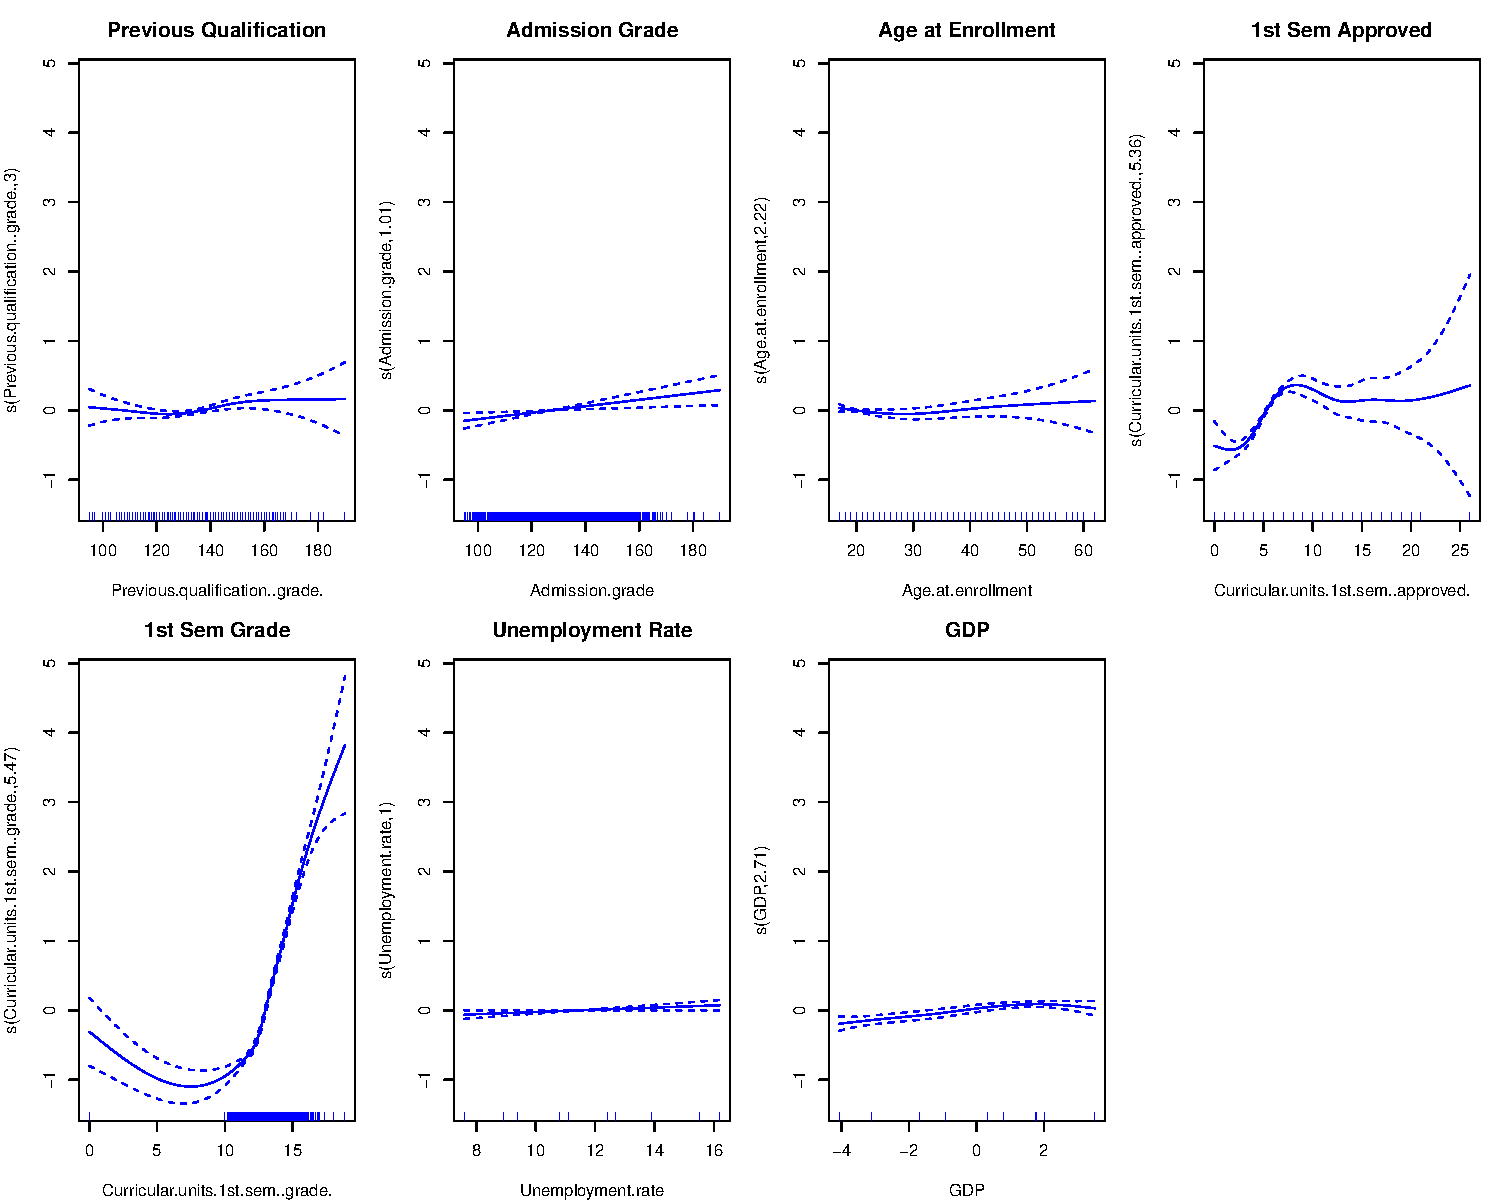
\includegraphics{final_report_ml1_group_files/figure-latex/gam1-smooth-1} 

}

\caption{Smooth functions reveal non-linear patterns}\label{fig:gam1-smooth}
\end{figure}

\textbf{Key Non-Linear Patterns:} Age effects may show optimal ranges,
course load might reveal sweet spots, and economic variables might
display threshold effects that linear models cannot capture.

\begin{Shaded}
\begin{Highlighting}[]
\FunctionTok{par}\NormalTok{(}\AttributeTok{mfrow =} \FunctionTok{c}\NormalTok{(}\DecValTok{1}\NormalTok{, }\DecValTok{2}\NormalTok{))}

\FunctionTok{plot}\NormalTok{(test\_g[[TARGET\_GRADE]], pred\_test\_g,}
     \AttributeTok{pch =} \DecValTok{16}\NormalTok{, }\AttributeTok{col =} \FunctionTok{rgb}\NormalTok{(}\FloatTok{0.5}\NormalTok{, }\DecValTok{0}\NormalTok{, }\FloatTok{0.5}\NormalTok{, }\FloatTok{0.5}\NormalTok{),}
     \AttributeTok{xlab =} \StringTok{"Actual Grade"}\NormalTok{, }\AttributeTok{ylab =} \StringTok{"Predicted Grade"}\NormalTok{,}
     \AttributeTok{main =} \FunctionTok{sprintf}\NormalTok{(}\StringTok{"GAM Predictions (R² = \%.4f)"}\NormalTok{, test\_r2\_g),}
     \AttributeTok{cex.main =} \FloatTok{1.3}\NormalTok{)}
\FunctionTok{abline}\NormalTok{(}\DecValTok{0}\NormalTok{, }\DecValTok{1}\NormalTok{, }\AttributeTok{col =} \StringTok{"red"}\NormalTok{, }\AttributeTok{lwd =} \DecValTok{2}\NormalTok{, }\AttributeTok{lty =} \DecValTok{2}\NormalTok{)}
\FunctionTok{grid}\NormalTok{()}

\NormalTok{residuals\_g }\OtherTok{\textless{}{-}}\NormalTok{ test\_g[[TARGET\_GRADE]] }\SpecialCharTok{{-}}\NormalTok{ pred\_test\_g}
\FunctionTok{plot}\NormalTok{(pred\_test\_g, residuals\_g,}
     \AttributeTok{pch =} \DecValTok{16}\NormalTok{, }\AttributeTok{col =} \FunctionTok{rgb}\NormalTok{(}\FloatTok{0.5}\NormalTok{, }\DecValTok{0}\NormalTok{, }\FloatTok{0.5}\NormalTok{, }\FloatTok{0.5}\NormalTok{),}
     \AttributeTok{xlab =} \StringTok{"Predicted Grade"}\NormalTok{, }\AttributeTok{ylab =} \StringTok{"Residuals"}\NormalTok{,}
     \AttributeTok{main =} \StringTok{"Residual Plot"}\NormalTok{,}
     \AttributeTok{cex.main =} \FloatTok{1.3}\NormalTok{)}
\FunctionTok{abline}\NormalTok{(}\AttributeTok{h =} \DecValTok{0}\NormalTok{, }\AttributeTok{col =} \StringTok{"red"}\NormalTok{, }\AttributeTok{lwd =} \DecValTok{2}\NormalTok{, }\AttributeTok{lty =} \DecValTok{2}\NormalTok{)}
\FunctionTok{grid}\NormalTok{()}
\end{Highlighting}
\end{Shaded}

\begin{figure}

{\centering 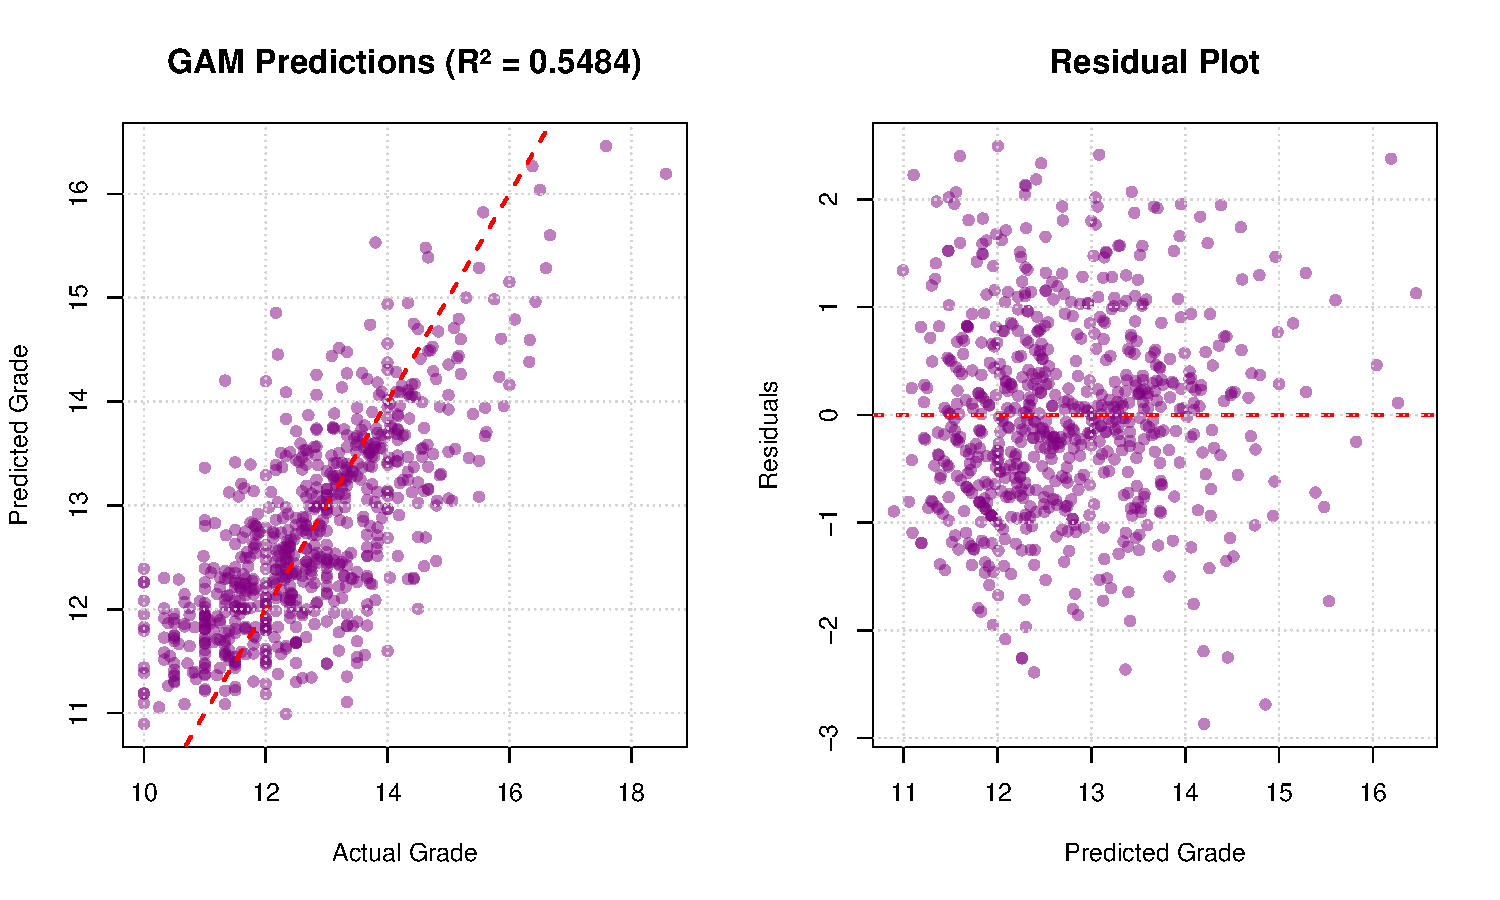
\includegraphics{final_report_ml1_group_files/figure-latex/gam1-predictions-1} 

}

\caption{GAM predictions maintain strong accuracy}\label{fig:gam1-predictions}
\end{figure}

\subsection{7.3 Model 2: Logistic GAM for Graduation
Prediction}\label{model-2-logistic-gam-for-graduation-prediction}

\begin{Shaded}
\begin{Highlighting}[]
\NormalTok{df\_success }\OtherTok{\textless{}{-}}\NormalTok{ df }\SpecialCharTok{\%\textgreater{}\%}
  \FunctionTok{filter}\NormalTok{(Target }\SpecialCharTok{\%in\%} \FunctionTok{c}\NormalTok{(}\StringTok{\textquotesingle{}Graduate\textquotesingle{}}\NormalTok{, }\StringTok{\textquotesingle{}Dropout\textquotesingle{}}\NormalTok{)) }\SpecialCharTok{\%\textgreater{}\%}
  \FunctionTok{mutate}\NormalTok{(}\AttributeTok{Success =} \FunctionTok{ifelse}\NormalTok{(Target }\SpecialCharTok{==} \StringTok{\textquotesingle{}Graduate\textquotesingle{}}\NormalTok{, }\DecValTok{1}\NormalTok{, }\DecValTok{0}\NormalTok{))}

\NormalTok{features\_success }\OtherTok{\textless{}{-}} \FunctionTok{c}\NormalTok{(}
  \StringTok{\textquotesingle{}Admission.grade\textquotesingle{}}\NormalTok{,}
  \StringTok{\textquotesingle{}Age.at.enrollment\textquotesingle{}}\NormalTok{,}
  \StringTok{\textquotesingle{}Scholarship.holder\textquotesingle{}}\NormalTok{,}
  \StringTok{\textquotesingle{}Tuition.fees.up.to.date\textquotesingle{}}\NormalTok{,}
  \StringTok{\textquotesingle{}Curricular.units.1st.sem..approved.\textquotesingle{}}\NormalTok{,}
  \StringTok{\textquotesingle{}Curricular.units.1st.sem..grade.\textquotesingle{}}\NormalTok{,}
  \StringTok{\textquotesingle{}Unemployment.rate\textquotesingle{}}\NormalTok{,}
  \StringTok{\textquotesingle{}GDP\textquotesingle{}}
\NormalTok{)}

\NormalTok{df\_success\_model }\OtherTok{\textless{}{-}}\NormalTok{ df\_success }\SpecialCharTok{\%\textgreater{}\%}
\NormalTok{  dplyr}\SpecialCharTok{::}\FunctionTok{select}\NormalTok{(}\FunctionTok{all\_of}\NormalTok{(}\FunctionTok{c}\NormalTok{(features\_success, }\StringTok{\textquotesingle{}Success\textquotesingle{}}\NormalTok{))) }\SpecialCharTok{\%\textgreater{}\%}
  \FunctionTok{mutate}\NormalTok{(}\FunctionTok{across}\NormalTok{(}\FunctionTok{everything}\NormalTok{(), as.numeric)) }\SpecialCharTok{\%\textgreater{}\%}
  \FunctionTok{na.omit}\NormalTok{()}

\FunctionTok{set.seed}\NormalTok{(}\DecValTok{42}\NormalTok{)}
\NormalTok{train\_index\_s }\OtherTok{\textless{}{-}} \FunctionTok{createDataPartition}\NormalTok{(df\_success\_model}\SpecialCharTok{$}\NormalTok{Success, }\AttributeTok{p =} \FloatTok{0.8}\NormalTok{, }\AttributeTok{list =} \ConstantTok{FALSE}\NormalTok{)}
\NormalTok{train\_s }\OtherTok{\textless{}{-}}\NormalTok{ df\_success\_model[train\_index\_s, ]}
\NormalTok{test\_s }\OtherTok{\textless{}{-}}\NormalTok{ df\_success\_model[}\SpecialCharTok{{-}}\NormalTok{train\_index\_s, ]}

\NormalTok{gam\_success }\OtherTok{\textless{}{-}} \FunctionTok{gam}\NormalTok{(}
\NormalTok{  Success }\SpecialCharTok{\textasciitilde{}}
    \FunctionTok{s}\NormalTok{(Admission.grade, }\AttributeTok{bs =} \StringTok{"cr"}\NormalTok{, }\AttributeTok{k =} \DecValTok{10}\NormalTok{) }\SpecialCharTok{+}
    \FunctionTok{s}\NormalTok{(Age.at.enrollment, }\AttributeTok{bs =} \StringTok{"cr"}\NormalTok{, }\AttributeTok{k =} \DecValTok{8}\NormalTok{) }\SpecialCharTok{+}
    \FunctionTok{factor}\NormalTok{(Scholarship.holder) }\SpecialCharTok{+}
    \FunctionTok{factor}\NormalTok{(Tuition.fees.up.to.date) }\SpecialCharTok{+}
    \FunctionTok{s}\NormalTok{(Curricular.units}\FloatTok{.1}\NormalTok{st.sem..approved., }\AttributeTok{bs =} \StringTok{"cr"}\NormalTok{, }\AttributeTok{k =} \DecValTok{8}\NormalTok{) }\SpecialCharTok{+}
    \FunctionTok{s}\NormalTok{(Curricular.units}\FloatTok{.1}\NormalTok{st.sem..grade., }\AttributeTok{bs =} \StringTok{"cr"}\NormalTok{, }\AttributeTok{k =} \DecValTok{10}\NormalTok{) }\SpecialCharTok{+}
    \FunctionTok{s}\NormalTok{(Unemployment.rate, }\AttributeTok{bs =} \StringTok{"cr"}\NormalTok{, }\AttributeTok{k =} \DecValTok{8}\NormalTok{) }\SpecialCharTok{+}
    \FunctionTok{s}\NormalTok{(GDP, }\AttributeTok{bs =} \StringTok{"cr"}\NormalTok{, }\AttributeTok{k =} \DecValTok{8}\NormalTok{),}
  \AttributeTok{data =}\NormalTok{ train\_s,}
  \AttributeTok{family =} \FunctionTok{binomial}\NormalTok{(}\AttributeTok{link =} \StringTok{"logit"}\NormalTok{),}
  \AttributeTok{method =} \StringTok{"REML"}
\NormalTok{)}
\end{Highlighting}
\end{Shaded}

\begin{Shaded}
\begin{Highlighting}[]
\NormalTok{pred\_proba\_s }\OtherTok{\textless{}{-}} \FunctionTok{predict}\NormalTok{(gam\_success, test\_s, }\AttributeTok{type =} \StringTok{"response"}\NormalTok{)}
\NormalTok{pred\_s }\OtherTok{\textless{}{-}} \FunctionTok{ifelse}\NormalTok{(pred\_proba\_s }\SpecialCharTok{\textgreater{}} \FloatTok{0.5}\NormalTok{, }\DecValTok{1}\NormalTok{, }\DecValTok{0}\NormalTok{)}

\NormalTok{accuracy\_s }\OtherTok{\textless{}{-}} \FunctionTok{mean}\NormalTok{(pred\_s }\SpecialCharTok{==}\NormalTok{ test\_s}\SpecialCharTok{$}\NormalTok{Success)}
\NormalTok{roc\_s }\OtherTok{\textless{}{-}} \FunctionTok{roc}\NormalTok{(test\_s}\SpecialCharTok{$}\NormalTok{Success, pred\_proba\_s, }\AttributeTok{quiet =} \ConstantTok{TRUE}\NormalTok{)}
\NormalTok{auc\_s }\OtherTok{\textless{}{-}} \FunctionTok{auc}\NormalTok{(roc\_s)}

\FunctionTok{cat}\NormalTok{(}\FunctionTok{sprintf}\NormalTok{(}\StringTok{"Accuracy: \%.4f (\%.2f\%\%)}\SpecialCharTok{\textbackslash{}n}\StringTok{"}\NormalTok{, accuracy\_s, accuracy\_s }\SpecialCharTok{*} \DecValTok{100}\NormalTok{))}
\FunctionTok{cat}\NormalTok{(}\FunctionTok{sprintf}\NormalTok{(}\StringTok{"AUC{-}ROC: \%.4f}\SpecialCharTok{\textbackslash{}n}\StringTok{"}\NormalTok{, auc\_s))}
\end{Highlighting}
\end{Shaded}

For the graduation GAM, the test set results are \textbf{accuracy =
0.85} and \textbf{AUC = 0.906}.

\begin{Shaded}
\begin{Highlighting}[]
\NormalTok{log\_reg }\OtherTok{\textless{}{-}} \FunctionTok{glm}\NormalTok{(Success }\SpecialCharTok{\textasciitilde{}}\NormalTok{ ., }\AttributeTok{data =}\NormalTok{ train\_s, }\AttributeTok{family =}\NormalTok{ binomial)}
\NormalTok{log\_pred\_proba }\OtherTok{\textless{}{-}} \FunctionTok{predict}\NormalTok{(log\_reg, test\_s, }\AttributeTok{type =} \StringTok{"response"}\NormalTok{)}
\NormalTok{log\_roc }\OtherTok{\textless{}{-}} \FunctionTok{roc}\NormalTok{(test\_s}\SpecialCharTok{$}\NormalTok{Success, log\_pred\_proba, }\AttributeTok{quiet =} \ConstantTok{TRUE}\NormalTok{)}
\NormalTok{log\_auc }\OtherTok{\textless{}{-}} \FunctionTok{auc}\NormalTok{(log\_roc)}

\FunctionTok{cat}\NormalTok{(}\StringTok{"}\SpecialCharTok{\textbackslash{}n}\StringTok{Logistic GAM vs Logistic GLM:}\SpecialCharTok{\textbackslash{}n}\StringTok{"}\NormalTok{)}
\FunctionTok{cat}\NormalTok{(}\FunctionTok{sprintf}\NormalTok{(}\StringTok{"GAM AUC:         \%.4f}\SpecialCharTok{\textbackslash{}n}\StringTok{"}\NormalTok{, auc\_s))}
\FunctionTok{cat}\NormalTok{(}\FunctionTok{sprintf}\NormalTok{(}\StringTok{"Logistic GLM:    \%.4f}\SpecialCharTok{\textbackslash{}n}\StringTok{"}\NormalTok{, log\_auc))}
\FunctionTok{cat}\NormalTok{(}\FunctionTok{sprintf}\NormalTok{(}\StringTok{"Improvement:     \%.2f percentage points}\SpecialCharTok{\textbackslash{}n}\StringTok{"}\NormalTok{, (auc\_s }\SpecialCharTok{{-}}\NormalTok{ log\_auc) }\SpecialCharTok{*} \DecValTok{100}\NormalTok{))}
\end{Highlighting}
\end{Shaded}

The GAM's \textbf{AUC} of 0.9055 versus 0.883 for standard logistic
regression represents meaningful improvement for \textbf{intervention
decisions}.

\subsubsection{Non-Linear Risk Patterns}\label{non-linear-risk-patterns}

\begin{Shaded}
\begin{Highlighting}[]
\FunctionTok{par}\NormalTok{(}\AttributeTok{mfrow =} \FunctionTok{c}\NormalTok{(}\DecValTok{2}\NormalTok{, }\DecValTok{3}\NormalTok{), }\AttributeTok{mar =} \FunctionTok{c}\NormalTok{(}\DecValTok{4}\NormalTok{, }\DecValTok{4}\NormalTok{, }\DecValTok{3}\NormalTok{, }\DecValTok{1}\NormalTok{))}
\FunctionTok{plot}\NormalTok{(gam\_success, }\AttributeTok{select =} \DecValTok{1}\NormalTok{, }\AttributeTok{shade =} \ConstantTok{TRUE}\NormalTok{, }\AttributeTok{col =} \StringTok{"darkgreen"}\NormalTok{, }\AttributeTok{shade.col =} \StringTok{"lightgreen"}\NormalTok{,}
     \AttributeTok{main =} \StringTok{"Admission Grade"}\NormalTok{, }\AttributeTok{cex.main =} \FloatTok{1.2}\NormalTok{, }\AttributeTok{ylab =} \StringTok{"Log{-}Odds of Graduation"}\NormalTok{)}
\FunctionTok{plot}\NormalTok{(gam\_success, }\AttributeTok{select =} \DecValTok{2}\NormalTok{, }\AttributeTok{shade =} \ConstantTok{TRUE}\NormalTok{, }\AttributeTok{col =} \StringTok{"darkgreen"}\NormalTok{, }\AttributeTok{shade.col =} \StringTok{"lightgreen"}\NormalTok{,}
     \AttributeTok{main =} \StringTok{"Age at Enrollment"}\NormalTok{, }\AttributeTok{cex.main =} \FloatTok{1.2}\NormalTok{, }\AttributeTok{ylab =} \StringTok{"Log{-}Odds of Graduation"}\NormalTok{)}
\FunctionTok{plot}\NormalTok{(gam\_success, }\AttributeTok{select =} \DecValTok{3}\NormalTok{, }\AttributeTok{shade =} \ConstantTok{TRUE}\NormalTok{, }\AttributeTok{col =} \StringTok{"darkgreen"}\NormalTok{, }\AttributeTok{shade.col =} \StringTok{"lightgreen"}\NormalTok{,}
     \AttributeTok{main =} \StringTok{"1st Sem Approved"}\NormalTok{, }\AttributeTok{cex.main =} \FloatTok{1.2}\NormalTok{, }\AttributeTok{ylab =} \StringTok{"Log{-}Odds of Graduation"}\NormalTok{)}
\FunctionTok{plot}\NormalTok{(gam\_success, }\AttributeTok{select =} \DecValTok{4}\NormalTok{, }\AttributeTok{shade =} \ConstantTok{TRUE}\NormalTok{, }\AttributeTok{col =} \StringTok{"darkgreen"}\NormalTok{, }\AttributeTok{shade.col =} \StringTok{"lightgreen"}\NormalTok{,}
     \AttributeTok{main =} \StringTok{"1st Sem Grade"}\NormalTok{, }\AttributeTok{cex.main =} \FloatTok{1.2}\NormalTok{, }\AttributeTok{ylab =} \StringTok{"Log{-}Odds of Graduation"}\NormalTok{)}
\FunctionTok{plot}\NormalTok{(gam\_success, }\AttributeTok{select =} \DecValTok{5}\NormalTok{, }\AttributeTok{shade =} \ConstantTok{TRUE}\NormalTok{, }\AttributeTok{col =} \StringTok{"darkgreen"}\NormalTok{, }\AttributeTok{shade.col =} \StringTok{"lightgreen"}\NormalTok{,}
     \AttributeTok{main =} \StringTok{"Unemployment"}\NormalTok{, }\AttributeTok{cex.main =} \FloatTok{1.2}\NormalTok{, }\AttributeTok{ylab =} \StringTok{"Log{-}Odds of Graduation"}\NormalTok{)}
\FunctionTok{plot}\NormalTok{(gam\_success, }\AttributeTok{select =} \DecValTok{6}\NormalTok{, }\AttributeTok{shade =} \ConstantTok{TRUE}\NormalTok{, }\AttributeTok{col =} \StringTok{"darkgreen"}\NormalTok{, }\AttributeTok{shade.col =} \StringTok{"lightgreen"}\NormalTok{,}
     \AttributeTok{main =} \StringTok{"GDP"}\NormalTok{, }\AttributeTok{cex.main =} \FloatTok{1.2}\NormalTok{, }\AttributeTok{ylab =} \StringTok{"Log{-}Odds of Graduation"}\NormalTok{)}
\end{Highlighting}
\end{Shaded}

\begin{figure}

{\centering 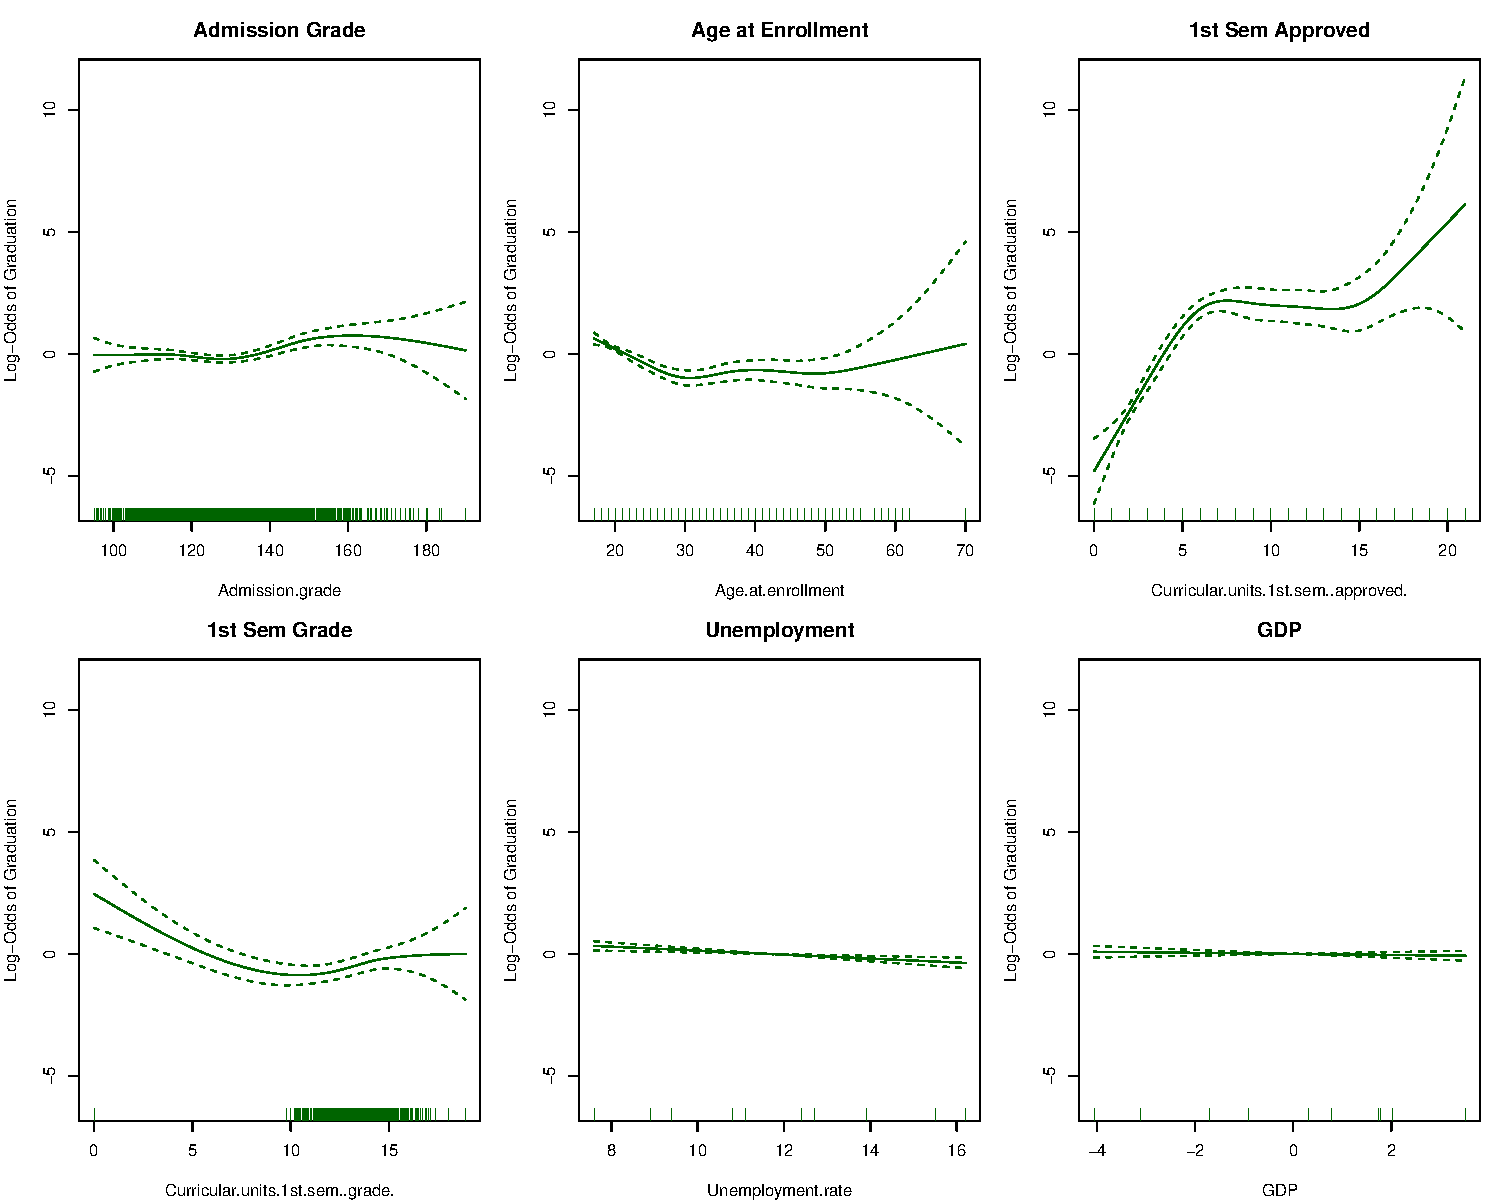
\includegraphics{final_report_ml1_group_files/figure-latex/gam2-smooth-1} 

}

\caption{Non-linear graduation probability patterns}\label{fig:gam2-smooth}
\end{figure}

\begin{Shaded}
\begin{Highlighting}[]
\FunctionTok{plot}\NormalTok{(roc\_s, }\AttributeTok{col =} \StringTok{"darkgreen"}\NormalTok{, }\AttributeTok{lwd =} \DecValTok{2}\NormalTok{,}
     \AttributeTok{main =} \FunctionTok{sprintf}\NormalTok{(}\StringTok{"ROC Curve {-} Logistic GAM (AUC = \%.3f)"}\NormalTok{, auc\_s),}
     \AttributeTok{cex.main =} \FloatTok{1.3}\NormalTok{)}
\FunctionTok{abline}\NormalTok{(}\AttributeTok{a =} \DecValTok{0}\NormalTok{, }\AttributeTok{b =} \DecValTok{1}\NormalTok{, }\AttributeTok{lty =} \DecValTok{2}\NormalTok{, }\AttributeTok{lwd =} \DecValTok{2}\NormalTok{, }\AttributeTok{col =} \StringTok{"black"}\NormalTok{)}
\FunctionTok{legend}\NormalTok{(}\StringTok{"bottomright"}\NormalTok{, }\AttributeTok{legend =} \FunctionTok{c}\NormalTok{(}\StringTok{"GAM"}\NormalTok{, }\StringTok{"Random"}\NormalTok{),}
       \AttributeTok{col =} \FunctionTok{c}\NormalTok{(}\StringTok{"darkgreen"}\NormalTok{, }\StringTok{"black"}\NormalTok{), }\AttributeTok{lwd =} \DecValTok{2}\NormalTok{, }\AttributeTok{lty =} \FunctionTok{c}\NormalTok{(}\DecValTok{1}\NormalTok{, }\DecValTok{2}\NormalTok{))}
\FunctionTok{grid}\NormalTok{()}
\end{Highlighting}
\end{Shaded}

\begin{figure}

{\centering 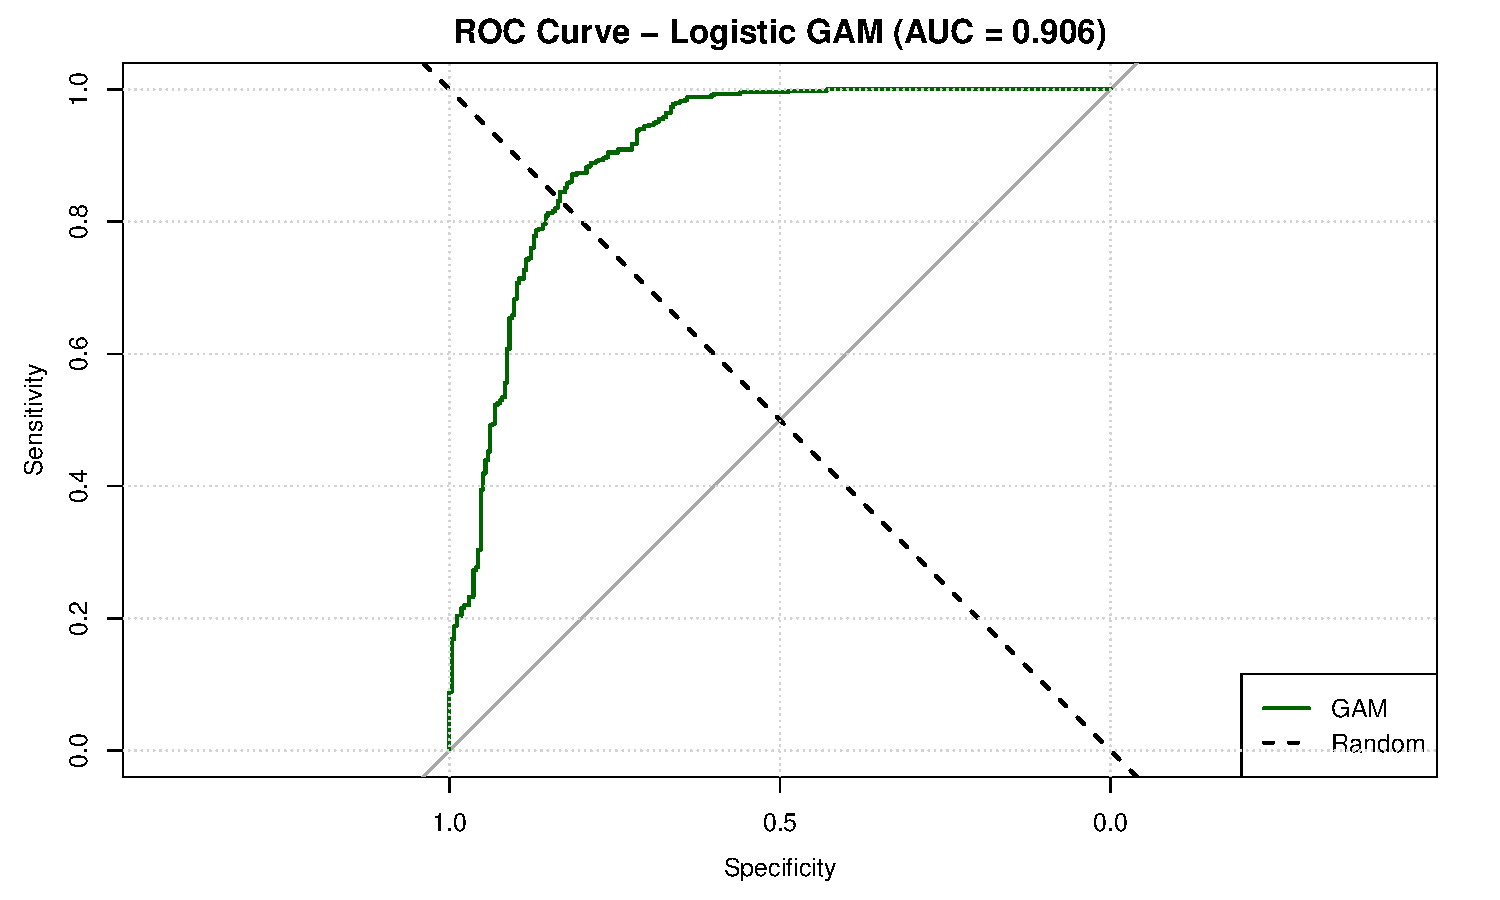
\includegraphics{final_report_ml1_group_files/figure-latex/gam2-roc-1} 

}

\caption{Logistic GAM achieves strong discrimination}\label{fig:gam2-roc}
\end{figure}

\subsection{7.4 Model 3: Poisson GAM for Course
Counts}\label{model-3-poisson-gam-for-course-counts}

For course count prediction, the Poisson GAM achieves \textbf{R² =
0.861} with \textbf{RMSE = 1.154} on the test set.

\subsubsection{Course Load Dynamics}\label{course-load-dynamics}

\begin{Shaded}
\begin{Highlighting}[]
\FunctionTok{par}\NormalTok{(}\AttributeTok{mfrow =} \FunctionTok{c}\NormalTok{(}\DecValTok{2}\NormalTok{, }\DecValTok{3}\NormalTok{), }\AttributeTok{mar =} \FunctionTok{c}\NormalTok{(}\DecValTok{4}\NormalTok{, }\DecValTok{4}\NormalTok{, }\DecValTok{3}\NormalTok{, }\DecValTok{1}\NormalTok{))}
\FunctionTok{plot}\NormalTok{(gam\_count, }\AttributeTok{select =} \DecValTok{1}\NormalTok{, }\AttributeTok{shade =} \ConstantTok{TRUE}\NormalTok{, }\AttributeTok{col =} \StringTok{"orange"}\NormalTok{, }\AttributeTok{shade.col =} \StringTok{"lightyellow"}\NormalTok{,}
     \AttributeTok{main =} \StringTok{"Admission Grade"}\NormalTok{, }\AttributeTok{cex.main =} \FloatTok{1.2}\NormalTok{, }\AttributeTok{ylab =} \StringTok{"Effect on Log(Count)"}\NormalTok{)}
\FunctionTok{plot}\NormalTok{(gam\_count, }\AttributeTok{select =} \DecValTok{2}\NormalTok{, }\AttributeTok{shade =} \ConstantTok{TRUE}\NormalTok{, }\AttributeTok{col =} \StringTok{"orange"}\NormalTok{, }\AttributeTok{shade.col =} \StringTok{"lightyellow"}\NormalTok{,}
     \AttributeTok{main =} \StringTok{"Age at Enrollment"}\NormalTok{, }\AttributeTok{cex.main =} \FloatTok{1.2}\NormalTok{, }\AttributeTok{ylab =} \StringTok{"Effect on Log(Count)"}\NormalTok{)}
\FunctionTok{plot}\NormalTok{(gam\_count, }\AttributeTok{select =} \DecValTok{3}\NormalTok{, }\AttributeTok{shade =} \ConstantTok{TRUE}\NormalTok{, }\AttributeTok{col =} \StringTok{"orange"}\NormalTok{, }\AttributeTok{shade.col =} \StringTok{"lightyellow"}\NormalTok{,}
     \AttributeTok{main =} \StringTok{"1st Sem Approved"}\NormalTok{, }\AttributeTok{cex.main =} \FloatTok{1.2}\NormalTok{, }\AttributeTok{ylab =} \StringTok{"Effect on Log(Count)"}\NormalTok{)}
\FunctionTok{plot}\NormalTok{(gam\_count, }\AttributeTok{select =} \DecValTok{4}\NormalTok{, }\AttributeTok{shade =} \ConstantTok{TRUE}\NormalTok{, }\AttributeTok{col =} \StringTok{"orange"}\NormalTok{, }\AttributeTok{shade.col =} \StringTok{"lightyellow"}\NormalTok{,}
     \AttributeTok{main =} \StringTok{"1st Sem Grade"}\NormalTok{, }\AttributeTok{cex.main =} \FloatTok{1.2}\NormalTok{, }\AttributeTok{ylab =} \StringTok{"Effect on Log(Count)"}\NormalTok{)}
\FunctionTok{plot}\NormalTok{(gam\_count, }\AttributeTok{select =} \DecValTok{5}\NormalTok{, }\AttributeTok{shade =} \ConstantTok{TRUE}\NormalTok{, }\AttributeTok{col =} \StringTok{"orange"}\NormalTok{, }\AttributeTok{shade.col =} \StringTok{"lightyellow"}\NormalTok{,}
     \AttributeTok{main =} \StringTok{"2nd Sem Enrolled"}\NormalTok{, }\AttributeTok{cex.main =} \FloatTok{1.2}\NormalTok{, }\AttributeTok{ylab =} \StringTok{"Effect on Log(Count)"}\NormalTok{)}
\end{Highlighting}
\end{Shaded}

\begin{figure}

{\centering 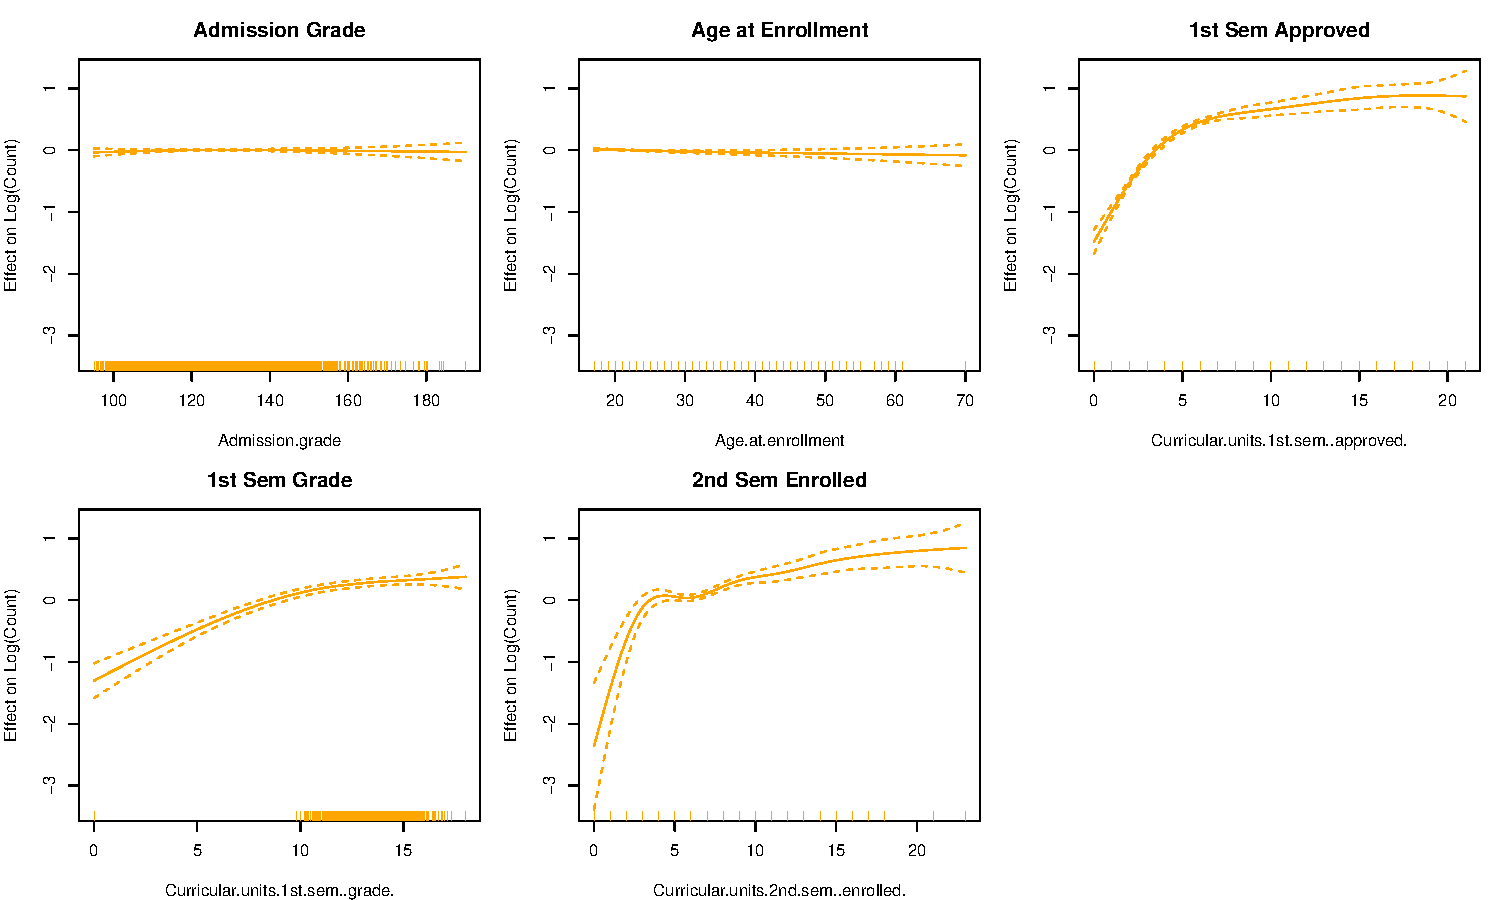
\includegraphics{final_report_ml1_group_files/figure-latex/gam3-smooth-1} 

}

\caption{Non-linear effects on course completion}\label{fig:gam3-smooth}
\end{figure}

\begin{Shaded}
\begin{Highlighting}[]
\FunctionTok{plot}\NormalTok{(test\_c[[TARGET\_COUNT]], pred\_test\_c,}
     \AttributeTok{pch =} \DecValTok{16}\NormalTok{, }\AttributeTok{col =} \FunctionTok{rgb}\NormalTok{(}\DecValTok{1}\NormalTok{, }\FloatTok{0.5}\NormalTok{, }\DecValTok{0}\NormalTok{, }\FloatTok{0.5}\NormalTok{),}
     \AttributeTok{xlab =} \StringTok{"Actual Courses Approved"}\NormalTok{, }\AttributeTok{ylab =} \StringTok{"Predicted Courses Approved"}\NormalTok{,}
     \AttributeTok{main =} \FunctionTok{sprintf}\NormalTok{(}\StringTok{"Poisson GAM (R² = \%.4f)"}\NormalTok{, test\_r2\_c),}
     \AttributeTok{cex.main =} \FloatTok{1.3}\NormalTok{, }\AttributeTok{cex.lab =} \FloatTok{1.1}\NormalTok{)}
\FunctionTok{abline}\NormalTok{(}\DecValTok{0}\NormalTok{, }\DecValTok{1}\NormalTok{, }\AttributeTok{col =} \StringTok{"red"}\NormalTok{, }\AttributeTok{lwd =} \DecValTok{2}\NormalTok{, }\AttributeTok{lty =} \DecValTok{2}\NormalTok{)}
\FunctionTok{grid}\NormalTok{()}
\end{Highlighting}
\end{Shaded}

\begin{figure}

{\centering 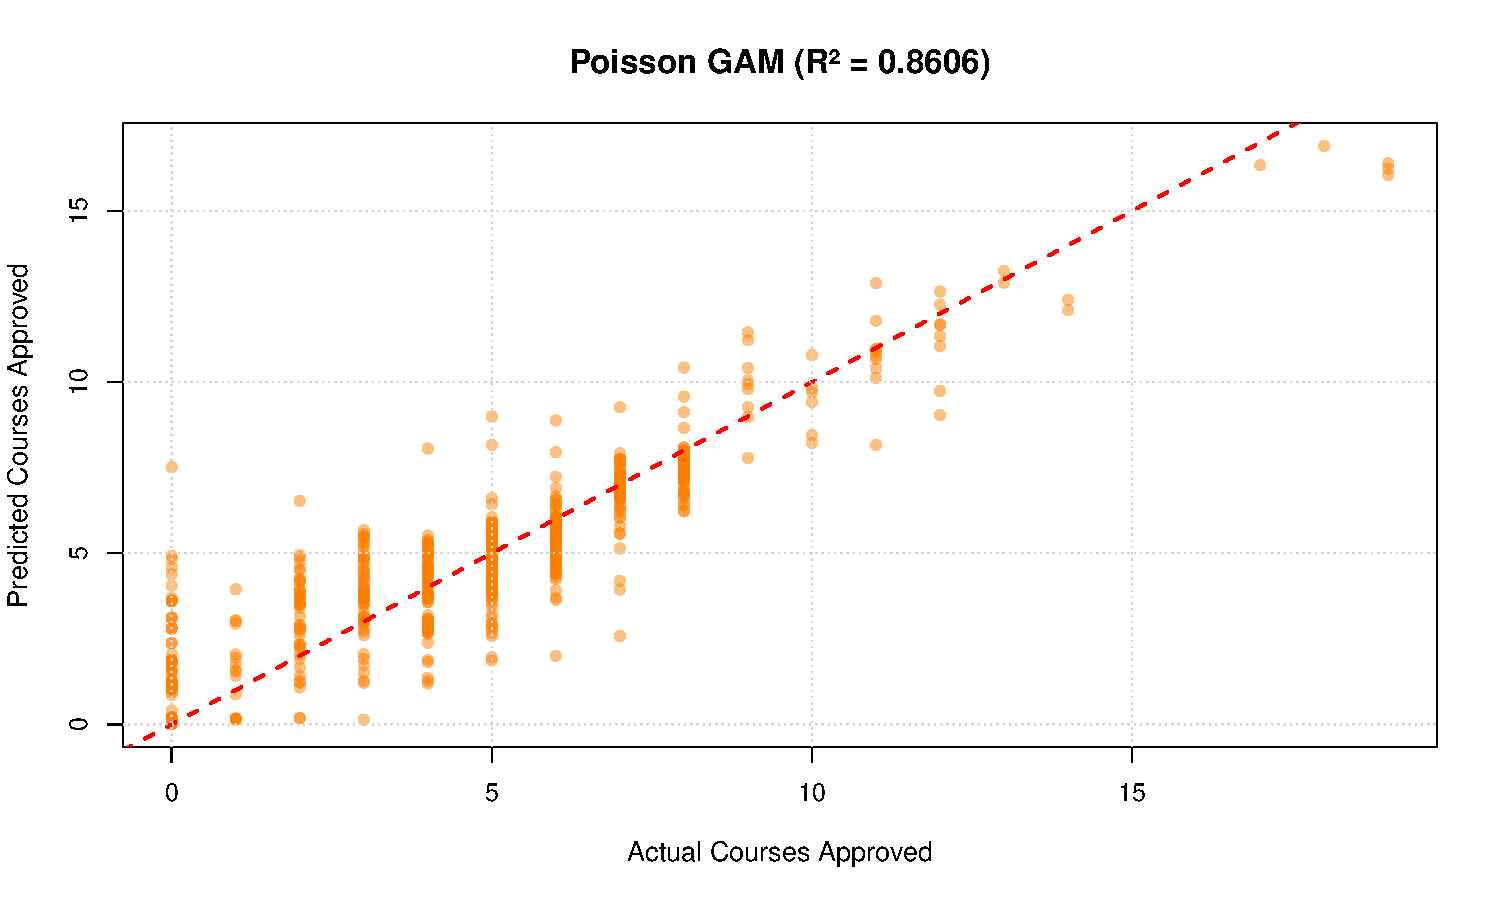
\includegraphics{final_report_ml1_group_files/figure-latex/gam3-predictions-1} 

}

\caption{Poisson GAM predictions}\label{fig:gam3-predictions}
\end{figure}

\begin{center}\rule{0.5\linewidth}{0.5pt}\end{center}

\section{8. Neural Network Analysis}\label{neural-network-analysis}

We use neural networks as an \textbf{early warning system} to predict
whether a student is at risk of \textbf{dropping out} (\textbf{Dropout
vs NotDropout}) based on early academic performance and financial
indicators. Here, \textbf{NotDropout} means the student is either
\textbf{still enrolled} or has \textbf{graduated}. The goal is not only
accuracy, but also \textbf{actionability}: the model should highlight
which signals (grades, approved courses, tuition status) are most
associated with dropout risk.

\subsection{8.1 Objective}\label{objective}

We want our neural network to play the role of an early-warning system:
predict \textbf{Dropout vs NotDropout} by learning the messy, non-linear
patterns hidden in the data.

\subsection{8.2 Feature Selection}\label{feature-selection}

We focus on three feature blocks from the preprocessed dataset:

\begin{enumerate}
\def\labelenumi{\arabic{enumi}.}
\tightlist
\item
  \textbf{Early academic performance:} 1st- and 2nd-semester grades plus
  approved credits showed the highest F-values in our ANOVA screening
  during preprocessing, making them the strongest predictors of the
  target variable.
\item
  \textbf{Financial pressure/support:} Tuition fees up to date, debtor
  status, and scholarship holder indicate whether financial stress may
  affect the student.
\item
  \textbf{Entry profile:} Admission grade and age at enrollment provide
  baseline information about the student's starting point.
\end{enumerate}

\subsection{8.3 Data Preprocessing for Neural
Networks}\label{data-preprocessing-for-neural-networks}

\begin{Shaded}
\begin{Highlighting}[]
\NormalTok{target\_counts }\OtherTok{\textless{}{-}}\NormalTok{ nn\_model\_data }\SpecialCharTok{\%\textgreater{}\%}
  \FunctionTok{count}\NormalTok{(Target) }\SpecialCharTok{\%\textgreater{}\%}
  \FunctionTok{mutate}\NormalTok{(}\AttributeTok{Percent =}\NormalTok{ n }\SpecialCharTok{/} \FunctionTok{sum}\NormalTok{(n) }\SpecialCharTok{*} \DecValTok{100}\NormalTok{)}

\FunctionTok{ggplot}\NormalTok{(target\_counts, }\FunctionTok{aes}\NormalTok{(}\AttributeTok{x =}\NormalTok{ Target, }\AttributeTok{y =}\NormalTok{ n, }\AttributeTok{fill =}\NormalTok{ Target)) }\SpecialCharTok{+}
  \FunctionTok{geom\_col}\NormalTok{(}\AttributeTok{alpha =} \FloatTok{0.85}\NormalTok{) }\SpecialCharTok{+}
  \FunctionTok{geom\_text}\NormalTok{(}\FunctionTok{aes}\NormalTok{(}\AttributeTok{label =} \FunctionTok{paste0}\NormalTok{(n, }\StringTok{" ("}\NormalTok{, }\FunctionTok{round}\NormalTok{(Percent, }\DecValTok{1}\NormalTok{), }\StringTok{"\%)"}\NormalTok{)), }\AttributeTok{vjust =} \SpecialCharTok{{-}}\FloatTok{0.3}\NormalTok{, }\AttributeTok{size =} \DecValTok{4}\NormalTok{) }\SpecialCharTok{+}
  \FunctionTok{scale\_fill\_manual}\NormalTok{(}\AttributeTok{values =} \FunctionTok{c}\NormalTok{(}\StringTok{"Dropout"} \OtherTok{=} \StringTok{"\#E74C3C"}\NormalTok{, }\StringTok{"NotDropout"} \OtherTok{=} \StringTok{"\#27AE60"}\NormalTok{)) }\SpecialCharTok{+}
  \FunctionTok{labs}\NormalTok{(}
    \AttributeTok{title =} \StringTok{"Target distribution in the neural network dataset"}\NormalTok{,}
    \AttributeTok{x =} \ConstantTok{NULL}\NormalTok{,}
    \AttributeTok{y =} \StringTok{"Number of students"}
\NormalTok{  ) }\SpecialCharTok{+}
  \FunctionTok{theme}\NormalTok{(}\AttributeTok{legend.position =} \StringTok{"none"}\NormalTok{)}
\end{Highlighting}
\end{Shaded}

\begin{center}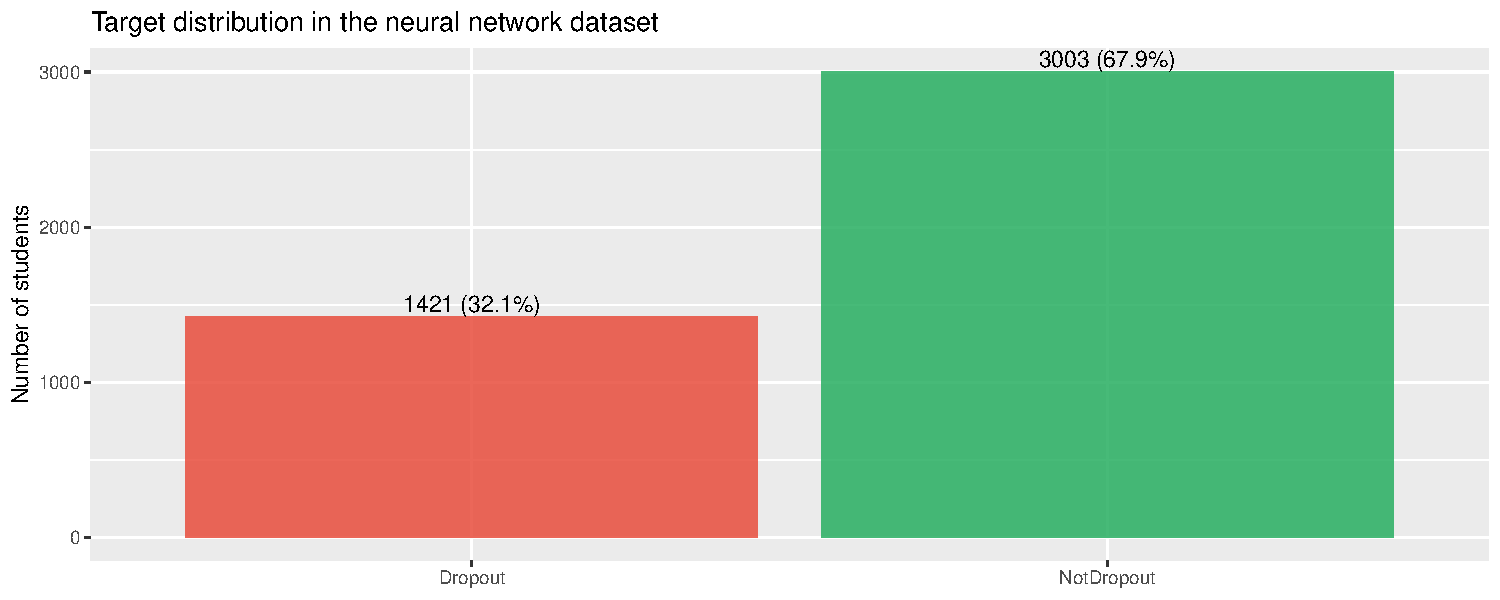
\includegraphics{final_report_ml1_group_files/figure-latex/nn-data-overview-1} \end{center}

This modeling subset contains \textbf{4424} students after removing
missing values. The chart above shows the class balance.

\subsection{8.4 Train/Test Split}\label{traintest-split}

\begin{Shaded}
\begin{Highlighting}[]
\FunctionTok{set.seed}\NormalTok{(}\DecValTok{123}\NormalTok{)}
\NormalTok{train\_idx }\OtherTok{\textless{}{-}} \FunctionTok{createDataPartition}\NormalTok{(nn\_model\_data}\SpecialCharTok{$}\NormalTok{Target, }\AttributeTok{p =} \FloatTok{0.8}\NormalTok{, }\AttributeTok{list =} \ConstantTok{FALSE}\NormalTok{)}
\NormalTok{train\_nn }\OtherTok{\textless{}{-}}\NormalTok{ nn\_model\_data[train\_idx, ]}
\NormalTok{test\_nn }\OtherTok{\textless{}{-}}\NormalTok{ nn\_model\_data[}\SpecialCharTok{{-}}\NormalTok{train\_idx, ]}
\end{Highlighting}
\end{Shaded}

We use an \textbf{80/20 split}: training = \textbf{3540}, test =
\textbf{884}.

\subsection{8.5 Model Training}\label{model-training}

We train two neural networks to compare Lab 1 and Lab 2 approaches.

\subsubsection{Model A: Single Hidden Layer (Lab 1 -
nnet)}\label{model-a-single-hidden-layer-lab-1---nnet}

Following \texttt{ANN\_Lab1\_GermanCredit\_v1.Rmd}, we use \texttt{nnet}
with one hidden layer and weight decay.

\begin{Shaded}
\begin{Highlighting}[]
\CommentTok{\# Model A: nnet with single hidden layer (Lab 1 style)}
\NormalTok{model\_A }\OtherTok{\textless{}{-}} \FunctionTok{nnet}\NormalTok{(}
\NormalTok{  Target }\SpecialCharTok{\textasciitilde{}}\NormalTok{ .,}
  \AttributeTok{data =}\NormalTok{ train\_nn,}
  \AttributeTok{size =} \DecValTok{10}\NormalTok{,        }\CommentTok{\# 10 hidden neurons in one layer}
  \AttributeTok{decay =} \FloatTok{0.01}\NormalTok{,     }\CommentTok{\# Weight decay: small penalty on large weights to prevent overfitting}
  \AttributeTok{maxit =} \DecValTok{500}\NormalTok{,      }\CommentTok{\# Maximum training iterations}
  \AttributeTok{trace =} \ConstantTok{FALSE}     \CommentTok{\# Suppress training progress output}
\NormalTok{)}
\end{Highlighting}
\end{Shaded}

\subsubsection{Model B: Three Hidden Layers (Lab 2 -
neuralnet)}\label{model-b-three-hidden-layers-lab-2---neuralnet}

Following \texttt{ANN\_Lab2\_Iris\_v1.Rmd}, we use \texttt{neuralnet}
with a deeper architecture using \textbf{three hidden layers}. This
requires numeric inputs and numeric output columns, so we build 0/1
columns for our binary target.

In this run, Model B uses a \textbf{2-5-2} hidden-layer setup (2 neurons
→ 5 neurons → 2 neurons). We also set \texttt{threshold\ =\ 0.8} mainly
to keep runtime manageable while we debug and iterate. A \textbf{larger}
threshold usually stops earlier (faster), but it can also stop before
the model has learned enough.

\begin{Shaded}
\begin{Highlighting}[]
\CommentTok{\# One{-}hot encode predictors for neuralnet (Lab 2 approach)}
\NormalTok{dummies }\OtherTok{\textless{}{-}} \FunctionTok{dummyVars}\NormalTok{(Target }\SpecialCharTok{\textasciitilde{}}\NormalTok{ ., }\AttributeTok{data =}\NormalTok{ train\_nn)}
\NormalTok{train\_matrix }\OtherTok{\textless{}{-}} \FunctionTok{as.data.frame}\NormalTok{(}\FunctionTok{predict}\NormalTok{(dummies, }\AttributeTok{newdata =}\NormalTok{ train\_nn))}
\NormalTok{test\_matrix }\OtherTok{\textless{}{-}} \FunctionTok{as.data.frame}\NormalTok{(}\FunctionTok{predict}\NormalTok{(dummies, }\AttributeTok{newdata =}\NormalTok{ test\_nn))}

\CommentTok{\# Create dummy columns for binary target (neuralnet needs numeric output)}
\NormalTok{train\_matrix}\SpecialCharTok{$}\NormalTok{Target\_Dropout }\OtherTok{\textless{}{-}} \FunctionTok{as.numeric}\NormalTok{(train\_nn}\SpecialCharTok{$}\NormalTok{Target }\SpecialCharTok{==} \StringTok{"Dropout"}\NormalTok{)}
\NormalTok{train\_matrix}\SpecialCharTok{$}\NormalTok{Target\_NotDropout }\OtherTok{\textless{}{-}} \FunctionTok{as.numeric}\NormalTok{(train\_nn}\SpecialCharTok{$}\NormalTok{Target }\SpecialCharTok{==} \StringTok{"NotDropout"}\NormalTok{)}

\CommentTok{\# Build formula: output columns \textasciitilde{} input columns}
\NormalTok{input\_names }\OtherTok{\textless{}{-}} \FunctionTok{names}\NormalTok{(train\_matrix)[}\SpecialCharTok{!}\FunctionTok{grepl}\NormalTok{(}\StringTok{"Target"}\NormalTok{, }\FunctionTok{names}\NormalTok{(train\_matrix))]}
\NormalTok{output\_names }\OtherTok{\textless{}{-}} \FunctionTok{c}\NormalTok{(}\StringTok{"Target\_Dropout"}\NormalTok{, }\StringTok{"Target\_NotDropout"}\NormalTok{)}
\NormalTok{formula\_B }\OtherTok{\textless{}{-}} \FunctionTok{as.formula}\NormalTok{(}\FunctionTok{paste}\NormalTok{(}
  \FunctionTok{paste}\NormalTok{(output\_names, }\AttributeTok{collapse =} \StringTok{" + "}\NormalTok{), }\StringTok{"\textasciitilde{}"}\NormalTok{,}
  \FunctionTok{paste}\NormalTok{(input\_names, }\AttributeTok{collapse =} \StringTok{" + "}\NormalTok{)}
\NormalTok{))}

\CommentTok{\# Model B: neuralnet with three hidden layers (Lab 2 style)}
\NormalTok{model\_B }\OtherTok{\textless{}{-}} \FunctionTok{neuralnet}\NormalTok{(}
\NormalTok{  formula\_B,}
  \AttributeTok{data =}\NormalTok{ train\_matrix,}
  \AttributeTok{hidden =} \FunctionTok{c}\NormalTok{(}\DecValTok{2}\NormalTok{,}\DecValTok{5}\NormalTok{,}\DecValTok{2}\NormalTok{),   }
  \AttributeTok{linear.output =} \ConstantTok{FALSE}\NormalTok{,}
  \AttributeTok{threshold =} \FloatTok{0.8}\NormalTok{, }
  \AttributeTok{stepmax =} \FloatTok{3e5}      \CommentTok{\# enough iterations without being too slow}
\NormalTok{)}
\end{Highlighting}
\end{Shaded}

\subsection{8.6 Model Evaluation}\label{model-evaluation}

We generate predictions and confusion matrices for both models.

\begin{Shaded}
\begin{Highlighting}[]
\CommentTok{\# {-}{-}{-} Model A predictions (nnet) {-}{-}{-}}
\NormalTok{pred\_A\_class }\OtherTok{\textless{}{-}} \FunctionTok{predict}\NormalTok{(model\_A, }\AttributeTok{newdata =}\NormalTok{ test\_nn, }\AttributeTok{type =} \StringTok{"class"}\NormalTok{)}
\NormalTok{pred\_A\_class }\OtherTok{\textless{}{-}} \FunctionTok{factor}\NormalTok{(pred\_A\_class, }\AttributeTok{levels =} \FunctionTok{levels}\NormalTok{(test\_nn}\SpecialCharTok{$}\NormalTok{Target))}
\NormalTok{conf\_matrix\_A }\OtherTok{\textless{}{-}} \FunctionTok{confusionMatrix}\NormalTok{(pred\_A\_class, test\_nn}\SpecialCharTok{$}\NormalTok{Target)}

\CommentTok{\# {-}{-}{-} Model B predictions (neuralnet) {-}{-}{-}}
\CommentTok{\# compute() runs the network on new data and returns raw output values}
\CommentTok{\# Must convert to matrix (neuralnet requires numeric matrix, not data.frame)}
\NormalTok{pred\_B\_raw }\OtherTok{\textless{}{-}} \FunctionTok{compute}\NormalTok{(model\_B, }\FunctionTok{as.matrix}\NormalTok{(test\_matrix[, input\_names]))}\SpecialCharTok{$}\NormalTok{net.result}
\CommentTok{\# Pick the class with highest output value for each student}
\NormalTok{pred\_B\_class }\OtherTok{\textless{}{-}} \FunctionTok{factor}\NormalTok{(}
  \FunctionTok{c}\NormalTok{(}\StringTok{"Dropout"}\NormalTok{, }\StringTok{"NotDropout"}\NormalTok{)[}\FunctionTok{apply}\NormalTok{(pred\_B\_raw, }\DecValTok{1}\NormalTok{, which.max)],}
  \AttributeTok{levels =} \FunctionTok{c}\NormalTok{(}\StringTok{"Dropout"}\NormalTok{, }\StringTok{"NotDropout"}\NormalTok{)}
\NormalTok{)}
\NormalTok{conf\_matrix\_B }\OtherTok{\textless{}{-}} \FunctionTok{confusionMatrix}\NormalTok{(pred\_B\_class, test\_nn}\SpecialCharTok{$}\NormalTok{Target)}
\end{Highlighting}
\end{Shaded}

\subsection{8.7 Performance Metrics
Summary}\label{performance-metrics-summary}

We report common classification metrics for both models. In the binary
setting, we treat \textbf{Dropout} as the ``positive'' class (this
matches the business goal of flagging students who may need support).

\begin{Shaded}
\begin{Highlighting}[]
\NormalTok{nn\_metrics\_df }\OtherTok{\textless{}{-}} \FunctionTok{tibble}\NormalTok{(}
  \AttributeTok{Model =} \FunctionTok{c}\NormalTok{(}\StringTok{"Model A: nnet (1 hidden layer)"}\NormalTok{, }\StringTok{"Model B: neuralnet (3 hidden layers)"}\NormalTok{),}
  \AttributeTok{Accuracy =} \FunctionTok{c}\NormalTok{(}
    \FunctionTok{as.numeric}\NormalTok{(conf\_matrix\_A}\SpecialCharTok{$}\NormalTok{overall[}\StringTok{"Accuracy"}\NormalTok{]),}
    \FunctionTok{as.numeric}\NormalTok{(conf\_matrix\_B}\SpecialCharTok{$}\NormalTok{overall[}\StringTok{"Accuracy"}\NormalTok{])}
\NormalTok{  ),}
  \AttributeTok{Precision =} \FunctionTok{c}\NormalTok{(}
    \FunctionTok{as.numeric}\NormalTok{(conf\_matrix\_A}\SpecialCharTok{$}\NormalTok{byClass[}\StringTok{"Pos Pred Value"}\NormalTok{]),}
    \FunctionTok{as.numeric}\NormalTok{(conf\_matrix\_B}\SpecialCharTok{$}\NormalTok{byClass[}\StringTok{"Pos Pred Value"}\NormalTok{])}
\NormalTok{  ),}
  \AttributeTok{Recall =} \FunctionTok{c}\NormalTok{(}
    \FunctionTok{as.numeric}\NormalTok{(conf\_matrix\_A}\SpecialCharTok{$}\NormalTok{byClass[}\StringTok{"Sensitivity"}\NormalTok{]),}
    \FunctionTok{as.numeric}\NormalTok{(conf\_matrix\_B}\SpecialCharTok{$}\NormalTok{byClass[}\StringTok{"Sensitivity"}\NormalTok{])}
\NormalTok{  )}
\NormalTok{)}
\end{Highlighting}
\end{Shaded}

\begin{Shaded}
\begin{Highlighting}[]
\NormalTok{nn\_metrics\_long }\OtherTok{\textless{}{-}}\NormalTok{ nn\_metrics\_df }\SpecialCharTok{\%\textgreater{}\%}
  \FunctionTok{pivot\_longer}\NormalTok{(}\AttributeTok{cols =} \FunctionTok{c}\NormalTok{(Accuracy, Precision, Recall), }\AttributeTok{names\_to =} \StringTok{"Metric"}\NormalTok{, }\AttributeTok{values\_to =} \StringTok{"Value"}\NormalTok{) }\SpecialCharTok{\%\textgreater{}\%}
  \FunctionTok{mutate}\NormalTok{(}
    \AttributeTok{Metric =} \FunctionTok{recode}\NormalTok{(}
\NormalTok{      Metric,}
      \AttributeTok{Accuracy =} \StringTok{"Accuracy"}\NormalTok{,}
      \AttributeTok{Precision =} \StringTok{"Precision (Dropout)"}\NormalTok{,}
      \AttributeTok{Recall =} \StringTok{"Recall (Dropout)"}
\NormalTok{    )}
\NormalTok{  )}

\FunctionTok{ggplot}\NormalTok{(nn\_metrics\_long, }\FunctionTok{aes}\NormalTok{(}\AttributeTok{x =}\NormalTok{ Metric, }\AttributeTok{y =}\NormalTok{ Value, }\AttributeTok{fill =}\NormalTok{ Model)) }\SpecialCharTok{+}
  \FunctionTok{geom\_col}\NormalTok{(}\AttributeTok{position =} \FunctionTok{position\_dodge}\NormalTok{(}\AttributeTok{width =} \FloatTok{0.75}\NormalTok{), }\AttributeTok{width =} \FloatTok{0.65}\NormalTok{, }\AttributeTok{alpha =} \FloatTok{0.9}\NormalTok{) }\SpecialCharTok{+}
  \FunctionTok{geom\_text}\NormalTok{(}
    \FunctionTok{aes}\NormalTok{(}\AttributeTok{label =} \FunctionTok{sprintf}\NormalTok{(}\StringTok{"\%.3f"}\NormalTok{, Value)),}
    \AttributeTok{position =} \FunctionTok{position\_dodge}\NormalTok{(}\AttributeTok{width =} \FloatTok{0.75}\NormalTok{),}
    \AttributeTok{vjust =} \SpecialCharTok{{-}}\FloatTok{0.4}\NormalTok{,}
    \AttributeTok{size =} \DecValTok{4}
\NormalTok{  ) }\SpecialCharTok{+}
  \FunctionTok{scale\_y\_continuous}\NormalTok{(}\AttributeTok{limits =} \FunctionTok{c}\NormalTok{(}\DecValTok{0}\NormalTok{, }\DecValTok{1}\NormalTok{), }\AttributeTok{labels =}\NormalTok{ scales}\SpecialCharTok{::}\FunctionTok{percent\_format}\NormalTok{(}\AttributeTok{accuracy =} \DecValTok{1}\NormalTok{)) }\SpecialCharTok{+}
  \FunctionTok{scale\_fill\_manual}\NormalTok{(}\AttributeTok{values =} \FunctionTok{c}\NormalTok{(}\StringTok{"\#5DADE2"}\NormalTok{, }\StringTok{"\#48C9B0"}\NormalTok{)) }\SpecialCharTok{+}
  \FunctionTok{labs}\NormalTok{(}
    \AttributeTok{title =} \StringTok{"Neural network performance on the test set"}\NormalTok{,}
    \AttributeTok{x =} \ConstantTok{NULL}\NormalTok{,}
    \AttributeTok{y =} \StringTok{"Score"}\NormalTok{,}
    \AttributeTok{fill =} \StringTok{"Model"}
\NormalTok{  ) }\SpecialCharTok{+}
  \FunctionTok{theme}\NormalTok{(}\AttributeTok{legend.position =} \StringTok{"top"}\NormalTok{)}
\end{Highlighting}
\end{Shaded}

\begin{center}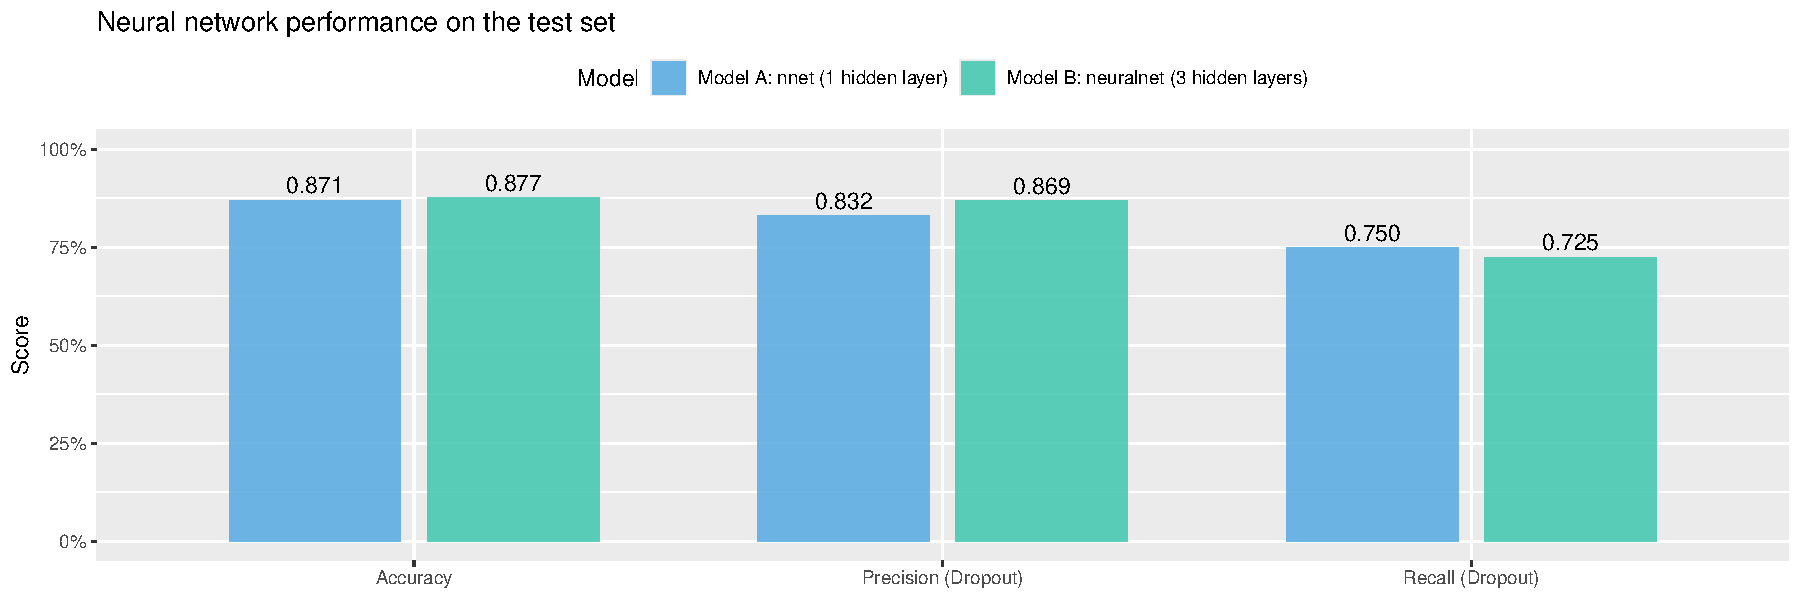
\includegraphics{final_report_ml1_group_files/figure-latex/nn-performance-dashboard-1} \end{center}

Model A (1 layer) still delivers the strongest result on the test set.
The deeper Model B (hidden layers: 2-5-2) does not automatically
outperform the simpler Model A. This mirrors the lecture message that
more layers are not automatically better for structured tabular data.

\subsection{8.8 Confusion Matrix
Comparison}\label{confusion-matrix-comparison}

Side-by-side heatmaps comparing both models. X-axis (top) = Predicted,
Y-axis = True labels.

\begin{Shaded}
\begin{Highlighting}[]
\CommentTok{\# Helper function to create confusion matrix plot}
\NormalTok{nn\_plot\_confusion\_matrix }\OtherTok{\textless{}{-}} \ControlFlowTok{function}\NormalTok{(conf\_matrix, title) \{}
\NormalTok{  cm\_df }\OtherTok{\textless{}{-}} \FunctionTok{as.data.frame}\NormalTok{(conf\_matrix}\SpecialCharTok{$}\NormalTok{table)}
  \FunctionTok{names}\NormalTok{(cm\_df) }\OtherTok{\textless{}{-}} \FunctionTok{c}\NormalTok{(}\StringTok{"Predicted"}\NormalTok{, }\StringTok{"True"}\NormalTok{, }\StringTok{"Count"}\NormalTok{)}
  
  \FunctionTok{ggplot}\NormalTok{(cm\_df, }\FunctionTok{aes}\NormalTok{(}\AttributeTok{x =}\NormalTok{ Predicted, }\AttributeTok{y =}\NormalTok{ True, }\AttributeTok{fill =}\NormalTok{ Count)) }\SpecialCharTok{+}
    \FunctionTok{geom\_tile}\NormalTok{(}\AttributeTok{color =} \StringTok{"white"}\NormalTok{, }\AttributeTok{linewidth =} \DecValTok{1}\NormalTok{) }\SpecialCharTok{+}
    \FunctionTok{geom\_text}\NormalTok{(}\FunctionTok{aes}\NormalTok{(}\AttributeTok{label =}\NormalTok{ Count), }\AttributeTok{size =} \DecValTok{5}\NormalTok{, }\AttributeTok{fontface =} \StringTok{"bold"}\NormalTok{, }\AttributeTok{color =} \StringTok{"white"}\NormalTok{) }\SpecialCharTok{+}
    \FunctionTok{scale\_fill\_gradient}\NormalTok{(}\AttributeTok{low =} \StringTok{"\#3498DB"}\NormalTok{, }\AttributeTok{high =} \StringTok{"\#E74C3C"}\NormalTok{, }\AttributeTok{name =} \StringTok{"Count"}\NormalTok{) }\SpecialCharTok{+}
    \FunctionTok{scale\_x\_discrete}\NormalTok{(}\AttributeTok{position =} \StringTok{"top"}\NormalTok{) }\SpecialCharTok{+}
    \FunctionTok{scale\_y\_discrete}\NormalTok{(}\AttributeTok{limits =} \FunctionTok{rev}\NormalTok{(}\FunctionTok{c}\NormalTok{(}\StringTok{"Dropout"}\NormalTok{, }\StringTok{"NotDropout"}\NormalTok{))) }\SpecialCharTok{+}
    \FunctionTok{labs}\NormalTok{(}\AttributeTok{title =}\NormalTok{ title, }\AttributeTok{x =} \StringTok{"Predicted Class"}\NormalTok{, }\AttributeTok{y =} \StringTok{"True Class"}\NormalTok{) }\SpecialCharTok{+}
    \FunctionTok{theme}\NormalTok{(}
      \AttributeTok{plot.title =} \FunctionTok{element\_text}\NormalTok{(}\AttributeTok{hjust =} \FloatTok{0.5}\NormalTok{, }\AttributeTok{face =} \StringTok{"bold"}\NormalTok{, }\AttributeTok{size =} \DecValTok{13}\NormalTok{),}
      \AttributeTok{axis.text =} \FunctionTok{element\_text}\NormalTok{(}\AttributeTok{size =} \DecValTok{10}\NormalTok{),}
      \AttributeTok{legend.position =} \StringTok{"right"}
\NormalTok{    )}
\NormalTok{\}}

\CommentTok{\# Create plots for both models}
\NormalTok{plot\_A }\OtherTok{\textless{}{-}} \FunctionTok{nn\_plot\_confusion\_matrix}\NormalTok{(conf\_matrix\_A, }\StringTok{"Model A: nnet (1 hidden layer)"}\NormalTok{)}
\NormalTok{plot\_B }\OtherTok{\textless{}{-}} \FunctionTok{nn\_plot\_confusion\_matrix}\NormalTok{(conf\_matrix\_B, }\StringTok{"Model B: neuralnet (3 hidden layers)"}\NormalTok{)}

\CommentTok{\# Display side by side}
\FunctionTok{grid.arrange}\NormalTok{(plot\_A, plot\_B, }\AttributeTok{ncol =} \DecValTok{2}\NormalTok{)}
\end{Highlighting}
\end{Shaded}

\begin{center}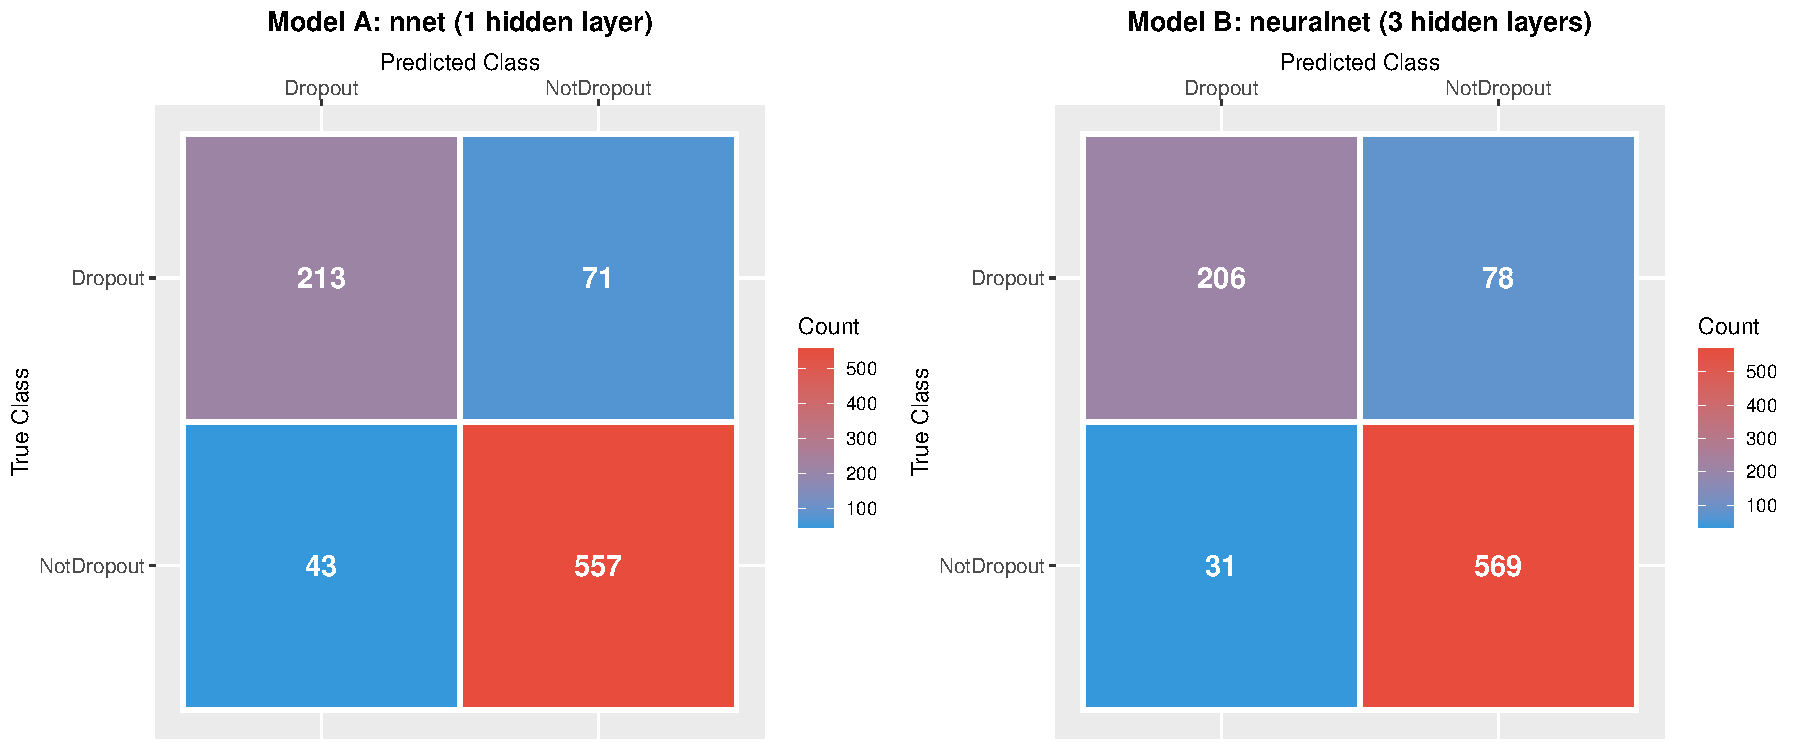
\includegraphics{final_report_ml1_group_files/figure-latex/nn-confusion-matrix-comparison-1} \end{center}

\subsection{8.9 ROC Curve Comparison}\label{roc-curve-comparison}

We compare ROC curves for \textbf{Dropout} (Dropout vs NotDropout)
across both models using \texttt{ROCR}.

\begin{Shaded}
\begin{Highlighting}[]
\CommentTok{\# {-}{-}{-} Model A ROC (nnet) {-}{-}{-}}
\NormalTok{prob\_A }\OtherTok{\textless{}{-}} \FunctionTok{predict}\NormalTok{(model\_A, }\AttributeTok{newdata =}\NormalTok{ test\_nn, }\AttributeTok{type =} \StringTok{"raw"}\NormalTok{)}

\CommentTok{\# Safety: nnet with binary target outputs P(Class 2), which is NotDropout.}
\CommentTok{\# We need P(Dropout).}
\ControlFlowTok{if}\NormalTok{ (}\FunctionTok{is.null}\NormalTok{(}\FunctionTok{dim}\NormalTok{(prob\_A)) }\SpecialCharTok{||} \FunctionTok{ncol}\NormalTok{(prob\_A) }\SpecialCharTok{==} \DecValTok{1}\NormalTok{) \{}
\NormalTok{  prob\_A\_drop }\OtherTok{\textless{}{-}} \DecValTok{1} \SpecialCharTok{{-}} \FunctionTok{as.numeric}\NormalTok{(prob\_A)}
\NormalTok{\} }\ControlFlowTok{else} \ControlFlowTok{if}\NormalTok{ (}\StringTok{"Dropout"} \SpecialCharTok{\%in\%} \FunctionTok{colnames}\NormalTok{(prob\_A)) \{}
\NormalTok{  prob\_A\_drop }\OtherTok{\textless{}{-}}\NormalTok{ prob\_A[, }\StringTok{"Dropout"}\NormalTok{]}
\NormalTok{\} }\ControlFlowTok{else}\NormalTok{ \{}
\NormalTok{  prob\_A\_drop }\OtherTok{\textless{}{-}}\NormalTok{ prob\_A[, }\DecValTok{1}\NormalTok{]}
\NormalTok{\}}

\NormalTok{pred\_A\_drop }\OtherTok{\textless{}{-}}\NormalTok{ ROCR}\SpecialCharTok{::}\FunctionTok{prediction}\NormalTok{(prob\_A\_drop, test\_nn}\SpecialCharTok{$}\NormalTok{Target }\SpecialCharTok{==} \StringTok{"Dropout"}\NormalTok{)}
\NormalTok{perf\_A\_drop }\OtherTok{\textless{}{-}}\NormalTok{ ROCR}\SpecialCharTok{::}\FunctionTok{performance}\NormalTok{(pred\_A\_drop, }\StringTok{"tpr"}\NormalTok{, }\StringTok{"fpr"}\NormalTok{)}
\NormalTok{auc\_A }\OtherTok{\textless{}{-}} \FunctionTok{round}\NormalTok{(ROCR}\SpecialCharTok{::}\FunctionTok{performance}\NormalTok{(pred\_A\_drop, }\StringTok{"auc"}\NormalTok{)}\SpecialCharTok{@}\NormalTok{y.values[[}\DecValTok{1}\NormalTok{]], }\DecValTok{3}\NormalTok{)}

\CommentTok{\# {-}{-}{-} Model B ROC (neuralnet) {-}{-}{-}}
\ControlFlowTok{if}\NormalTok{ (}\FunctionTok{is.null}\NormalTok{(}\FunctionTok{dim}\NormalTok{(pred\_B\_raw))) \{}
\NormalTok{  prob\_B\_drop }\OtherTok{\textless{}{-}} \FunctionTok{as.numeric}\NormalTok{(pred\_B\_raw)}
\NormalTok{\} }\ControlFlowTok{else}\NormalTok{ \{}
\NormalTok{  prob\_B\_drop }\OtherTok{\textless{}{-}}\NormalTok{ pred\_B\_raw[, }\DecValTok{1}\NormalTok{]}
\NormalTok{\}}
\NormalTok{pred\_B\_drop }\OtherTok{\textless{}{-}}\NormalTok{ ROCR}\SpecialCharTok{::}\FunctionTok{prediction}\NormalTok{(prob\_B\_drop, test\_nn}\SpecialCharTok{$}\NormalTok{Target }\SpecialCharTok{==} \StringTok{"Dropout"}\NormalTok{)}
\NormalTok{perf\_B\_drop }\OtherTok{\textless{}{-}}\NormalTok{ ROCR}\SpecialCharTok{::}\FunctionTok{performance}\NormalTok{(pred\_B\_drop, }\StringTok{"tpr"}\NormalTok{, }\StringTok{"fpr"}\NormalTok{)}
\NormalTok{auc\_B }\OtherTok{\textless{}{-}} \FunctionTok{round}\NormalTok{(ROCR}\SpecialCharTok{::}\FunctionTok{performance}\NormalTok{(pred\_B\_drop, }\StringTok{"auc"}\NormalTok{)}\SpecialCharTok{@}\NormalTok{y.values[[}\DecValTok{1}\NormalTok{]], }\DecValTok{3}\NormalTok{)}
\end{Highlighting}
\end{Shaded}

\begin{Shaded}
\begin{Highlighting}[]
\NormalTok{roc\_A\_df }\OtherTok{\textless{}{-}} \FunctionTok{data.frame}\NormalTok{(}
  \AttributeTok{FPR =}\NormalTok{ perf\_A\_drop}\SpecialCharTok{@}\NormalTok{x.values[[}\DecValTok{1}\NormalTok{]],}
  \AttributeTok{TPR =}\NormalTok{ perf\_A\_drop}\SpecialCharTok{@}\NormalTok{y.values[[}\DecValTok{1}\NormalTok{]],}
  \AttributeTok{Model =} \FunctionTok{sprintf}\NormalTok{(}\StringTok{"Model A (AUC=\%.3f)"}\NormalTok{, auc\_A)}
\NormalTok{)}
\NormalTok{roc\_B\_df }\OtherTok{\textless{}{-}} \FunctionTok{data.frame}\NormalTok{(}
  \AttributeTok{FPR =}\NormalTok{ perf\_B\_drop}\SpecialCharTok{@}\NormalTok{x.values[[}\DecValTok{1}\NormalTok{]],}
  \AttributeTok{TPR =}\NormalTok{ perf\_B\_drop}\SpecialCharTok{@}\NormalTok{y.values[[}\DecValTok{1}\NormalTok{]],}
  \AttributeTok{Model =} \FunctionTok{sprintf}\NormalTok{(}\StringTok{"Model B (AUC=\%.3f)"}\NormalTok{, auc\_B)}
\NormalTok{)}
\NormalTok{roc\_df }\OtherTok{\textless{}{-}} \FunctionTok{bind\_rows}\NormalTok{(roc\_A\_df, roc\_B\_df)}

\FunctionTok{ggplot}\NormalTok{(roc\_df, }\FunctionTok{aes}\NormalTok{(}\AttributeTok{x =}\NormalTok{ FPR, }\AttributeTok{y =}\NormalTok{ TPR, }\AttributeTok{color =}\NormalTok{ Model)) }\SpecialCharTok{+}
  \FunctionTok{geom\_line}\NormalTok{(}\AttributeTok{linewidth =} \FloatTok{1.2}\NormalTok{) }\SpecialCharTok{+}
  \FunctionTok{geom\_abline}\NormalTok{(}\AttributeTok{slope =} \DecValTok{1}\NormalTok{, }\AttributeTok{intercept =} \DecValTok{0}\NormalTok{, }\AttributeTok{linetype =} \DecValTok{2}\NormalTok{, }\AttributeTok{color =} \StringTok{"gray50"}\NormalTok{) }\SpecialCharTok{+}
  \FunctionTok{scale\_color\_manual}\NormalTok{(}\AttributeTok{values =} \FunctionTok{c}\NormalTok{(}\StringTok{"\#2ecc71"}\NormalTok{, }\StringTok{"\#3498db"}\NormalTok{)) }\SpecialCharTok{+}
  \FunctionTok{labs}\NormalTok{(}
    \AttributeTok{title =} \StringTok{"ROC curve (Dropout vs NotDropout)"}\NormalTok{,}
    \AttributeTok{x =} \StringTok{"False Positive Rate"}\NormalTok{,}
    \AttributeTok{y =} \StringTok{"True Positive Rate"}\NormalTok{,}
    \AttributeTok{color =} \ConstantTok{NULL}
\NormalTok{  ) }\SpecialCharTok{+}
  \FunctionTok{theme}\NormalTok{(}\AttributeTok{legend.position =} \StringTok{"bottom"}\NormalTok{)}
\end{Highlighting}
\end{Shaded}

\begin{center}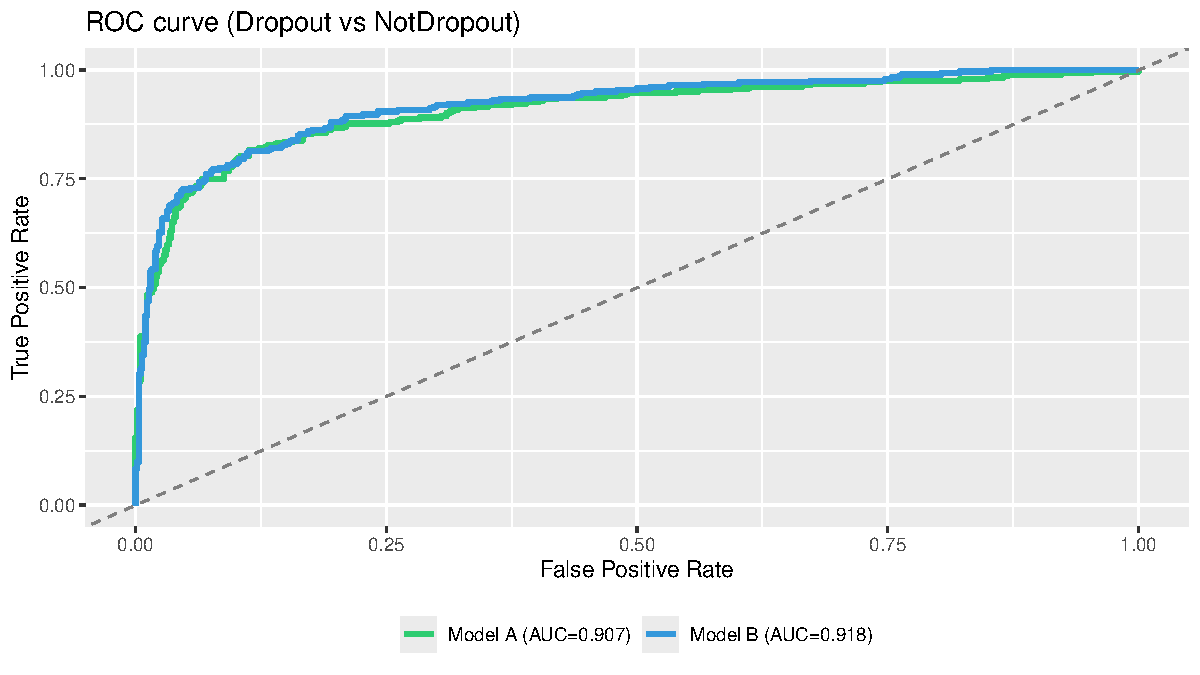
\includegraphics{final_report_ml1_group_files/figure-latex/nn-roc-comparison-plot-1} \end{center}

\textbf{AUC interpretation:} higher AUC means better separation of
Dropout vs NotDropout. Here, Model A has AUC \textbf{0.907} and Model B
has AUC \textbf{0.918}. But \textbf{the difference is minimal}.

\subsection{8.10 Feature Importance
(Permutation)}\label{feature-importance-permutation}

Permutation importance (same spirit as Lab 1's ``what-if'' checks)
measures how much each \emph{model's accuracy} drops when we randomly
shuffle one predictor at a time. Bigger drops mean the learner
\emph{relied heavily on that feature}. It shows that \textbf{second
semester grades are a very important factor}. It is interesting that at
HSLU, we also feel like the \textbf{second semester is the hardest} and
requires a lot of \textbf{effort and attention}.

\begin{Shaded}
\begin{Highlighting}[]
\CommentTok{\# Helper to compute accuracy drop for a single feature and model}
\NormalTok{permute\_feature }\OtherTok{\textless{}{-}} \ControlFlowTok{function}\NormalTok{(model\_type, var\_name) \{}
\NormalTok{  permuted }\OtherTok{\textless{}{-}}\NormalTok{ test\_nn}
\NormalTok{  permuted[[var\_name]] }\OtherTok{\textless{}{-}} \FunctionTok{sample}\NormalTok{(permuted[[var\_name]])}
  
  \ControlFlowTok{if}\NormalTok{ (model\_type }\SpecialCharTok{==} \StringTok{"Model A: nnet (1 layer)"}\NormalTok{) \{}
\NormalTok{    baseline }\OtherTok{\textless{}{-}} \FunctionTok{mean}\NormalTok{(}\FunctionTok{predict}\NormalTok{(model\_A, }\AttributeTok{newdata =}\NormalTok{ test\_nn, }\AttributeTok{type =} \StringTok{"class"}\NormalTok{) }\SpecialCharTok{==}\NormalTok{ test\_nn}\SpecialCharTok{$}\NormalTok{Target)}
\NormalTok{    perm\_acc }\OtherTok{\textless{}{-}} \FunctionTok{mean}\NormalTok{(}\FunctionTok{predict}\NormalTok{(model\_A, }\AttributeTok{newdata =}\NormalTok{ permuted, }\AttributeTok{type =} \StringTok{"class"}\NormalTok{) }\SpecialCharTok{==}\NormalTok{ test\_nn}\SpecialCharTok{$}\NormalTok{Target)}
\NormalTok{  \} }\ControlFlowTok{else}\NormalTok{ \{}
\NormalTok{    permuted\_matrix }\OtherTok{\textless{}{-}} \FunctionTok{as.data.frame}\NormalTok{(}\FunctionTok{predict}\NormalTok{(dummies, }\AttributeTok{newdata =}\NormalTok{ permuted))}
\NormalTok{    permuted\_matrix[] }\OtherTok{\textless{}{-}} \FunctionTok{lapply}\NormalTok{(permuted\_matrix, as.numeric)}
\NormalTok{    class\_map }\OtherTok{\textless{}{-}} \FunctionTok{c}\NormalTok{(}\StringTok{"Dropout"}\NormalTok{, }\StringTok{"NotDropout"}\NormalTok{)}
\NormalTok{    baseline }\OtherTok{\textless{}{-}} \FunctionTok{mean}\NormalTok{(pred\_B\_class }\SpecialCharTok{==}\NormalTok{ test\_nn}\SpecialCharTok{$}\NormalTok{Target)}
\NormalTok{    perm\_raw }\OtherTok{\textless{}{-}} \FunctionTok{compute}\NormalTok{(model\_B, }\FunctionTok{as.matrix}\NormalTok{(permuted\_matrix[, input\_names]))}\SpecialCharTok{$}\NormalTok{net.result}
\NormalTok{    perm\_class }\OtherTok{\textless{}{-}} \FunctionTok{factor}\NormalTok{(class\_map[}\FunctionTok{apply}\NormalTok{(perm\_raw, }\DecValTok{1}\NormalTok{, which.max)], }\AttributeTok{levels =}\NormalTok{ class\_map)}
\NormalTok{    perm\_acc }\OtherTok{\textless{}{-}} \FunctionTok{mean}\NormalTok{(perm\_class }\SpecialCharTok{==}\NormalTok{ test\_nn}\SpecialCharTok{$}\NormalTok{Target)}
\NormalTok{  \}}
  
  \FunctionTok{tibble}\NormalTok{(}
    \AttributeTok{Model =}\NormalTok{ model\_type,}
    \AttributeTok{Feature =}\NormalTok{ var\_name,}
    \AttributeTok{AccuracyDrop =}\NormalTok{ baseline }\SpecialCharTok{{-}}\NormalTok{ perm\_acc}
\NormalTok{  )}
\NormalTok{\}}

\NormalTok{perm\_results }\OtherTok{\textless{}{-}} \FunctionTok{map\_dfr}\NormalTok{(}
\NormalTok{  nn\_features,}
  \SpecialCharTok{\textasciitilde{}}\FunctionTok{bind\_rows}\NormalTok{(}
    \FunctionTok{permute\_feature}\NormalTok{(}\StringTok{"Model A: nnet (1 layer)"}\NormalTok{, .x),}
    \FunctionTok{permute\_feature}\NormalTok{(}\StringTok{"Model B: neuralnet (3 layers)"}\NormalTok{, .x)}
\NormalTok{  )}
\NormalTok{)}

\CommentTok{\# Friendlier labels for the plot}
\NormalTok{feature\_labels }\OtherTok{\textless{}{-}} \FunctionTok{c}\NormalTok{(}
  \StringTok{"Curricular.units.1st.sem..approved."} \OtherTok{=} \StringTok{"1st Sem Credits Approved"}\NormalTok{,}
  \StringTok{"Curricular.units.1st.sem..grade."} \OtherTok{=} \StringTok{"1st Sem Grade"}\NormalTok{,}
  \StringTok{"Curricular.units.2nd.sem..approved."} \OtherTok{=} \StringTok{"2nd Sem Credits Approved"}\NormalTok{,}
  \StringTok{"Curricular.units.2nd.sem..grade."} \OtherTok{=} \StringTok{"2nd Sem Grade"}\NormalTok{,}
  \StringTok{"Tuition.fees.up.to.date"} \OtherTok{=} \StringTok{"Tuition Fees Up to Date"}\NormalTok{,}
  \StringTok{"Scholarship.holder"} \OtherTok{=} \StringTok{"Scholarship Holder"}\NormalTok{,}
  \StringTok{"Age.at.enrollment"} \OtherTok{=} \StringTok{"Age at Enrollment"}\NormalTok{,}
  \StringTok{"Admission.grade"} \OtherTok{=} \StringTok{"Admission Grade"}\NormalTok{,}
  \StringTok{"Debtor"} \OtherTok{=} \StringTok{"Debtor Status"}
\NormalTok{)}

\NormalTok{perm\_results }\OtherTok{\textless{}{-}}\NormalTok{ perm\_results }\SpecialCharTok{\%\textgreater{}\%}
  \FunctionTok{mutate}\NormalTok{(}\AttributeTok{Feature =} \FunctionTok{recode}\NormalTok{(Feature, }\SpecialCharTok{!!!}\NormalTok{feature\_labels)) }\SpecialCharTok{\%\textgreater{}\%}
  \FunctionTok{group\_by}\NormalTok{(Model) }\SpecialCharTok{\%\textgreater{}\%}
  \FunctionTok{mutate}\NormalTok{(}\AttributeTok{Feature =} \FunctionTok{fct\_reorder}\NormalTok{(Feature, AccuracyDrop)) }\SpecialCharTok{\%\textgreater{}\%}
  \FunctionTok{ungroup}\NormalTok{()}

\FunctionTok{ggplot}\NormalTok{(perm\_results, }\FunctionTok{aes}\NormalTok{(}\AttributeTok{x =}\NormalTok{ AccuracyDrop, }\AttributeTok{y =}\NormalTok{ Feature, }\AttributeTok{fill =}\NormalTok{ Model)) }\SpecialCharTok{+}
  \FunctionTok{geom\_col}\NormalTok{(}\AttributeTok{show.legend =} \ConstantTok{FALSE}\NormalTok{) }\SpecialCharTok{+}
  \FunctionTok{facet\_wrap}\NormalTok{(}\SpecialCharTok{\textasciitilde{}}\NormalTok{Model, }\AttributeTok{scales =} \StringTok{"free\_y"}\NormalTok{) }\SpecialCharTok{+}
  \FunctionTok{labs}\NormalTok{(}
    \AttributeTok{title =} \StringTok{"Permutation Importance (Accuracy Drop when Shuffled)"}\NormalTok{,}
    \AttributeTok{x =} \StringTok{"Accuracy Drop"}\NormalTok{,}
    \AttributeTok{y =} \StringTok{"Feature"}
\NormalTok{  ) }\SpecialCharTok{+}
  \FunctionTok{scale\_fill\_manual}\NormalTok{(}\AttributeTok{values =} \FunctionTok{c}\NormalTok{(}\StringTok{"\#5DADE2"}\NormalTok{, }\StringTok{"\#48C9B0"}\NormalTok{))}
\end{Highlighting}
\end{Shaded}

\begin{center}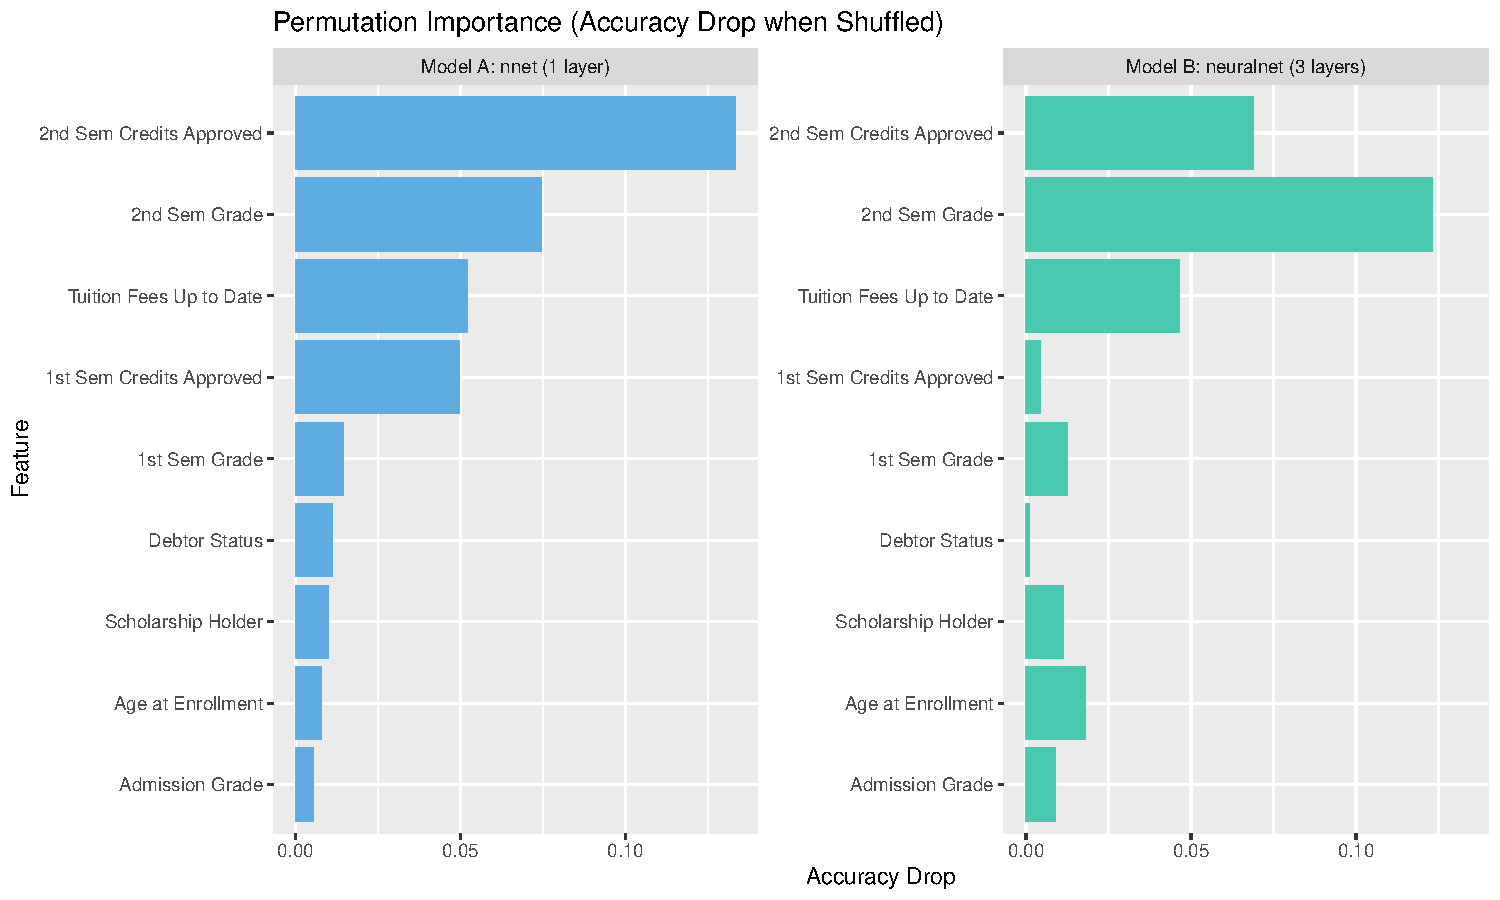
\includegraphics{final_report_ml1_group_files/figure-latex/nn-permutation-importance-1} \end{center}

\begin{Shaded}
\begin{Highlighting}[]
\NormalTok{perm\_top }\OtherTok{\textless{}{-}}\NormalTok{ perm\_results }\SpecialCharTok{\%\textgreater{}\%}
  \FunctionTok{group\_by}\NormalTok{(Model) }\SpecialCharTok{\%\textgreater{}\%}
  \FunctionTok{slice\_max}\NormalTok{(}\AttributeTok{order\_by =}\NormalTok{ AccuracyDrop, }\AttributeTok{n =} \DecValTok{5}\NormalTok{, }\AttributeTok{with\_ties =} \ConstantTok{FALSE}\NormalTok{) }\SpecialCharTok{\%\textgreater{}\%}
  \FunctionTok{ungroup}\NormalTok{() }\SpecialCharTok{\%\textgreater{}\%}
  \FunctionTok{mutate}\NormalTok{(}\AttributeTok{AccuracyDropPctPoints =} \FunctionTok{round}\NormalTok{(AccuracyDrop }\SpecialCharTok{*} \DecValTok{100}\NormalTok{, }\DecValTok{2}\NormalTok{)) }\SpecialCharTok{\%\textgreater{}\%}
  \FunctionTok{select}\NormalTok{(Model, Feature, AccuracyDropPctPoints)}

\NormalTok{knitr}\SpecialCharTok{::}\FunctionTok{kable}\NormalTok{(}
\NormalTok{  perm\_top,}
  \AttributeTok{caption =} \StringTok{"Top 5 permutation importances (how many accuracy percentage points we lose when we shuffle the feature)"}
\NormalTok{)}
\end{Highlighting}
\end{Shaded}

\begin{longtable}[]{@{}
  >{\raggedright\arraybackslash}p{(\linewidth - 4\tabcolsep) * \real{0.3896}}
  >{\raggedright\arraybackslash}p{(\linewidth - 4\tabcolsep) * \real{0.3247}}
  >{\raggedleft\arraybackslash}p{(\linewidth - 4\tabcolsep) * \real{0.2857}}@{}}
\caption{Top 5 permutation importances (how many accuracy percentage
points we lose when we shuffle the feature)}\tabularnewline
\toprule\noalign{}
\begin{minipage}[b]{\linewidth}\raggedright
Model
\end{minipage} & \begin{minipage}[b]{\linewidth}\raggedright
Feature
\end{minipage} & \begin{minipage}[b]{\linewidth}\raggedleft
AccuracyDropPctPoints
\end{minipage} \\
\midrule\noalign{}
\endfirsthead
\toprule\noalign{}
\begin{minipage}[b]{\linewidth}\raggedright
Model
\end{minipage} & \begin{minipage}[b]{\linewidth}\raggedright
Feature
\end{minipage} & \begin{minipage}[b]{\linewidth}\raggedleft
AccuracyDropPctPoints
\end{minipage} \\
\midrule\noalign{}
\endhead
\bottomrule\noalign{}
\endlastfoot
Model A: nnet (1 layer) & 2nd Sem Credits Approved & 13.35 \\
Model A: nnet (1 layer) & 2nd Sem Grade & 7.47 \\
Model A: nnet (1 layer) & Tuition Fees Up to Date & 5.20 \\
Model A: nnet (1 layer) & 1st Sem Credits Approved & 4.98 \\
Model A: nnet (1 layer) & 1st Sem Grade & 1.47 \\
Model B: neuralnet (3 layers) & 2nd Sem Grade & 12.33 \\
Model B: neuralnet (3 layers) & 2nd Sem Credits Approved & 6.90 \\
Model B: neuralnet (3 layers) & Tuition Fees Up to Date & 4.64 \\
Model B: neuralnet (3 layers) & Age at Enrollment & 1.81 \\
Model B: neuralnet (3 layers) & 1st Sem Grade & 1.24 \\
\end{longtable}

\subsection{8.11 Business Use: Early Warning and
Intervention}\label{business-use-early-warning-and-intervention}

This neural network can be used as an \textbf{early warning system}:

\begin{enumerate}
\def\labelenumi{\arabic{enumi}.}
\tightlist
\item
  At the end of the 1st/2nd semester, we collect the same inputs
  (grades, approved units, tuition status, scholarship, debtor status).
\item
  The model outputs a \textbf{dropout risk score} for each student (the
  model's predicted output/probability for the \textbf{Dropout} class).
\item
  The university can then \textbf{target limited support resources} to
  students with the highest predicted risk.
\end{enumerate}

Examples of interventions (linked to our most important features):

\begin{itemize}
\tightlist
\item
  \textbf{Academic performance signals (grades, approved units):}
  provide tutoring, mentoring, and early academic advising.
\item
  \textbf{Financial stress signals (tuition up to date, debtor):}
  proactive outreach about payment plans and financial aid options.
\item
  \textbf{Support signals (scholarship holder):} consider expanding
  support programs for similar students who are not currently covered.
\end{itemize}

Important caution:

\begin{itemize}
\tightlist
\item
  The model helps us \textbf{prioritize} students for support, but it
  should not be the only decision tool.
\item
  The safest process is to combine model predictions with human review
  (advisors) before taking action.
\end{itemize}

\subsection{8.12 Neural Network Architecture
Visualization}\label{neural-network-architecture-visualization}

\texttt{NeuralNetTools::plotnet()} turns the fitted networks into
diagrams that show layers, neurons, and connection strengths (thicker
lines = larger absolute weights).

\begin{Shaded}
\begin{Highlighting}[]
\NormalTok{short\_labels }\OtherTok{\textless{}{-}} \FunctionTok{c}\NormalTok{(}\StringTok{"1st}\SpecialCharTok{\textbackslash{}n}\StringTok{Credits"}\NormalTok{, }\StringTok{"1st}\SpecialCharTok{\textbackslash{}n}\StringTok{Grade"}\NormalTok{, }\StringTok{"2nd}\SpecialCharTok{\textbackslash{}n}\StringTok{Credits"}\NormalTok{, }\StringTok{"2nd}\SpecialCharTok{\textbackslash{}n}\StringTok{Grade"}\NormalTok{,}
                  \StringTok{"Tuition}\SpecialCharTok{\textbackslash{}n}\StringTok{OK"}\NormalTok{, }\StringTok{"Scholar"}\NormalTok{, }\StringTok{"Age"}\NormalTok{, }\StringTok{"Adm}\SpecialCharTok{\textbackslash{}n}\StringTok{Grade"}\NormalTok{, }\StringTok{"Debtor"}\NormalTok{)}
\NormalTok{output\_labels\_B }\OtherTok{\textless{}{-}} \FunctionTok{c}\NormalTok{(}\StringTok{"Dropout"}\NormalTok{, }\StringTok{"NotDropout"}\NormalTok{)}

\FunctionTok{par}\NormalTok{(}\AttributeTok{mfrow =} \FunctionTok{c}\NormalTok{(}\DecValTok{1}\NormalTok{, }\DecValTok{2}\NormalTok{), }\AttributeTok{mar =} \FunctionTok{c}\NormalTok{(}\DecValTok{2}\NormalTok{, }\DecValTok{2}\NormalTok{, }\DecValTok{2}\NormalTok{, }\DecValTok{2}\NormalTok{))}
\NormalTok{NeuralNetTools}\SpecialCharTok{::}\FunctionTok{plotnet}\NormalTok{(}
\NormalTok{  model\_A,}
  \AttributeTok{alpha =} \FloatTok{0.7}\NormalTok{,}
  \AttributeTok{circle\_col =} \FunctionTok{list}\NormalTok{(}\StringTok{"steelblue"}\NormalTok{, }\StringTok{"skyblue"}\NormalTok{),}
  \AttributeTok{x\_names =}\NormalTok{ short\_labels,}
  \AttributeTok{max\_sp =} \ConstantTok{TRUE}\NormalTok{,}
  \AttributeTok{cex\_val =} \FloatTok{0.9}\NormalTok{,}
  \AttributeTok{line\_lwd =} \FloatTok{0.8}
\NormalTok{)}
\NormalTok{NeuralNetTools}\SpecialCharTok{::}\FunctionTok{plotnet}\NormalTok{(}
\NormalTok{  model\_B,}
  \AttributeTok{alpha =} \FloatTok{0.7}\NormalTok{,}
  \AttributeTok{circle\_col =} \FunctionTok{list}\NormalTok{(}\StringTok{"darkseagreen"}\NormalTok{, }\StringTok{"palegreen"}\NormalTok{),}
  \AttributeTok{x\_names =}\NormalTok{ short\_labels,}
  \AttributeTok{y\_names =}\NormalTok{ output\_labels\_B,}
  \AttributeTok{max\_sp =} \ConstantTok{TRUE}\NormalTok{,}
  \AttributeTok{cex\_val =} \FloatTok{0.9}\NormalTok{,}
  \AttributeTok{line\_lwd =} \FloatTok{0.8}
\NormalTok{)}
\end{Highlighting}
\end{Shaded}

\begin{center}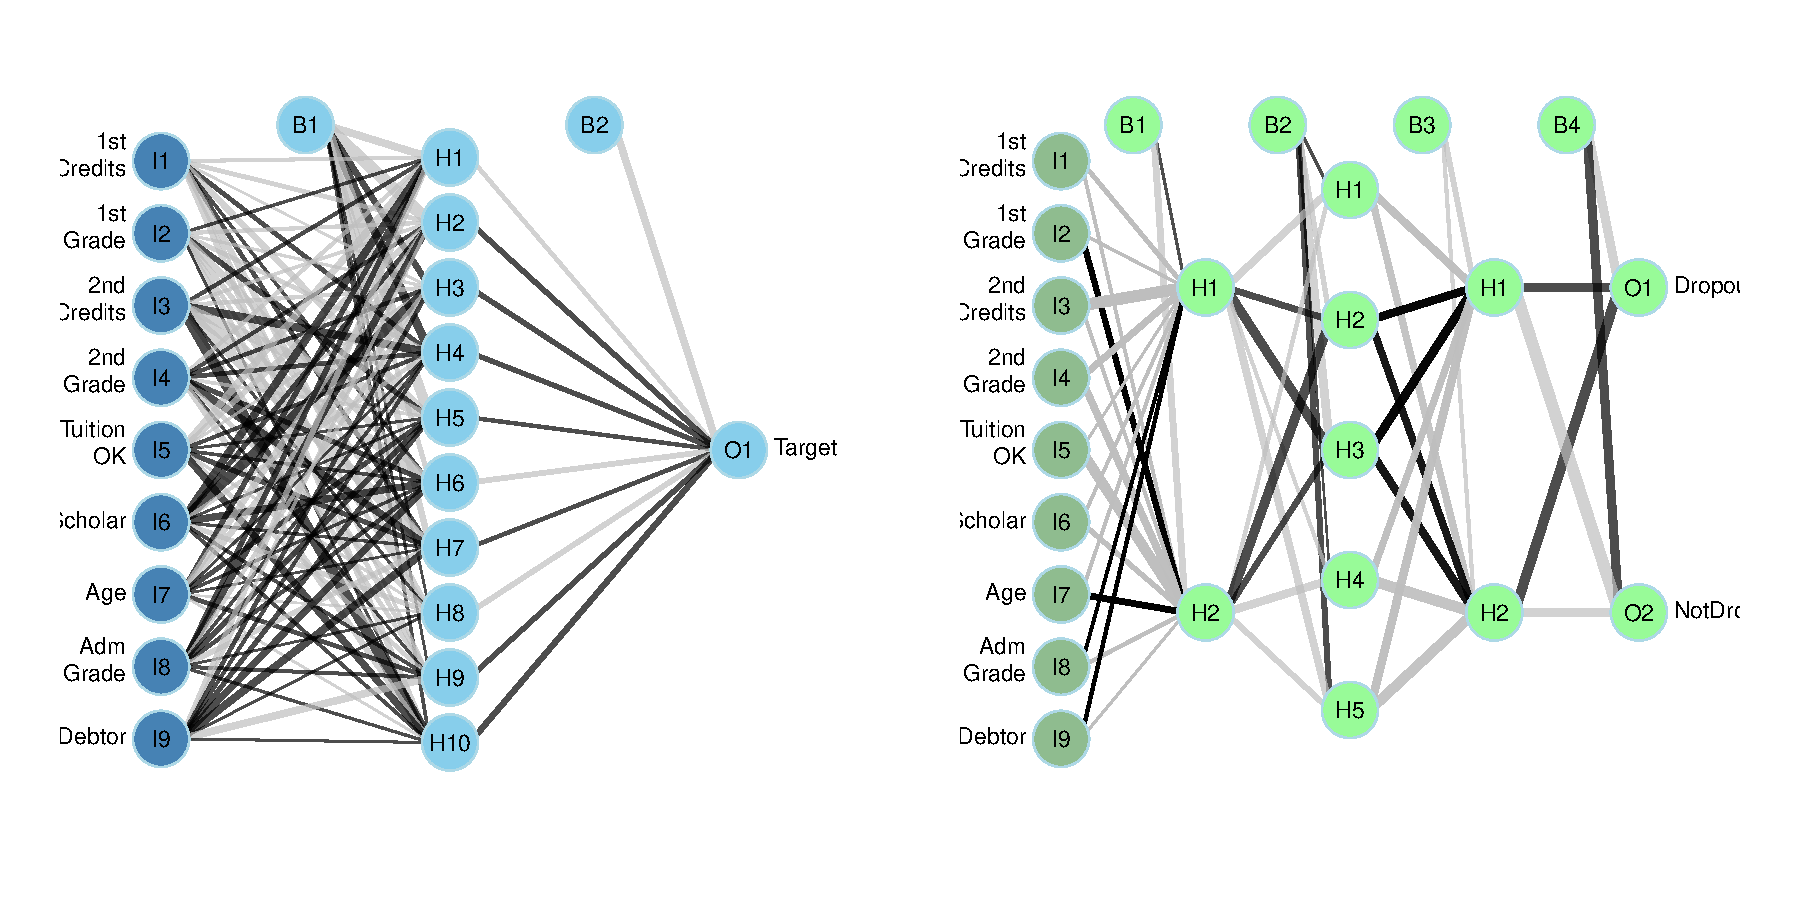
\includegraphics{final_report_ml1_group_files/figure-latex/nn-visualization-1} \end{center}

\begin{Shaded}
\begin{Highlighting}[]
\FunctionTok{par}\NormalTok{(}\AttributeTok{mfrow =} \FunctionTok{c}\NormalTok{(}\DecValTok{1}\NormalTok{, }\DecValTok{1}\NormalTok{))}
\end{Highlighting}
\end{Shaded}

\subsection{8.13 Findings \&
Interpretation}\label{findings-interpretation}

\textbf{Model A (nnet):} 9 inputs - 10 hidden neurons - 1 output
(P(NotDropout)). \textbf{Simple, fast}, handles factors directly and
reaches strong test performance.

\textbf{Model B (neuralnet):} 9 inputs - 2 - 5 - 2 neurons - 2 outputs.
Shows Lab 2's deeper setup but \textbf{does not automatically outperform
the simpler Model A}.

\textbf{Strengths observed:} Neural networks capture non-linear
interaction between grades, tuition status, and scholarships.

\textbf{Limitations observed:}

\begin{itemize}
\tightlist
\item
  Deeper networks remain sensitive to hyperparameters and can overfit
  small samples.
\item
  Interpretability is limited compared to GLM/GAM coefficients.
\item
  Because we combine \textbf{Enrolled + Graduate} into
  \textbf{NotDropout}, this target cannot distinguish ``still studying''
  from ``already graduated''. This is acceptable for an early-warning
  dropout use case, but it matters if the business question is
  specifically ``who will graduate''.
\end{itemize}

\subsection{8.14 Neural Network
Conclusions}\label{neural-network-conclusions}

\begin{enumerate}
\def\labelenumi{\arabic{enumi}.}
\tightlist
\item
  Both neural networks predict \textbf{dropout risk} reasonably well,
  but the single hidden layer (Model A) provides the best balance of
  accuracy and stability on this dataset.
\item
  Adding more layers (Model B: 2-5-2) does not automatically outperform
  the simpler architecture; this reinforces the lab insight that
  ``deeper'' is not automatically ``better'' for structured tabular
  data.
\item
  Standard preprocessing steps (scaling numeric features, stratified
  train/test split) remain essential for consistent results.
\end{enumerate}

\begin{center}\rule{0.5\linewidth}{0.5pt}\end{center}

\section{9. Support Vector Machine
Analysis}\label{support-vector-machine-analysis}

We will now test different vector models to understand what is the best
classifier for our student's performance. SVMs operate by identifying
where the \textbf{margin} between different categories of data is the
greatest. To classify our dataset, the model plots a separating line
between the two outcome classes using a number of predictors - in order
to keep it clear, we want to create a two-dimensional plane (two
predictors).

By applying different kernels---linear, radial, and polynomial--- we
assess how the shape of the decision boundary affects prediction
accuracy and determine which kernel provides the most reliable
classification for our dataset.

\subsection{Feature Selection}\label{feature-selection-1}

For us to choose the best predictors, we will compute
\textbf{F-statistic ANOVA} for every numeric feature in the dataset. The
F-score tell us \emph{how much} the mean of each feature differs between
the \textbf{two target groups} (\emph{Graduation}/\emph{Dropout}).
higher scores mean there is a bigger separation between classes, and a
better cutoff between groups. Results indicate that grades and the
amount of credits approved have the highest F-Values, suggesting they
are the most significant predictors for predicting the success of
graduating or not.

In this case, we want to choose the features of \textbf{second semester
marks} and the \textbf{amount of units passed} to plot our model.

\begin{longtable}[]{@{}lrl@{}}
\caption{Top 5 Features by F-statistic}\tabularnewline
\toprule\noalign{}
Feature & F\_value & p\_value \\
\midrule\noalign{}
\endfirsthead
\toprule\noalign{}
Feature & F\_value & p\_value \\
\midrule\noalign{}
\endhead
\bottomrule\noalign{}
\endlastfoot
Curricular.units.2nd.sem..approved. & 2711.44 & 0.000 \\
Curricular.units.2nd.sem..grade. & 2098.45 & 0.000 \\
Curricular.units.1st.sem..approved. & 1613.96 & 0.000 \\
Curricular.units.1st.sem..grade. & 1344.07 & 0.000 \\
Tuition.fees.up.to.date & 881.55 & 0.000 \\
\end{longtable}

\subsection{Prepare Data for SVM}\label{prepare-data-for-svm}

Support Vector Machines require \textbf{predictors} (numerical
variables) and a \textbf{target} (categorical:
\emph{Graduate}/\emph{Dropout}) for classification. The data was then
structured into a format suitable for SVM modeling. The original dataset
contained three academic outcomes: \emph{Enrolled}, \emph{Dropout}, and
\emph{Graduate}. Since the objective of this analysis is to distinguish
students who ultimately graduate from those who drop out, \textbf{the
Enrolled category was removed}. This reduces the dataset size but
produces a cleaner binary classification.

\begin{longtable}[]{@{}cc@{}}
\caption{Dataset Summary}\tabularnewline
\toprule\noalign{}
Metric & Value \\
\midrule\noalign{}
\endfirsthead
\toprule\noalign{}
Metric & Value \\
\midrule\noalign{}
\endhead
\bottomrule\noalign{}
\endlastfoot
Total Observations & 3630 \\
Target Classes & Dropout, Graduate \\
\end{longtable}

\subsection{Exploratory Visualization}\label{exploratory-visualization}

\subsection{Train/Test Split}\label{traintest-split-1}

Now, we will split the data into training and testing sets, and then fit
several SVM models to classify the students based on their marks.

\begin{longtable}[]{@{}ccc@{}}
\caption{Train/Test Split}\tabularnewline
\toprule\noalign{}
Dataset & Observations & Percentage \\
\midrule\noalign{}
\endfirsthead
\toprule\noalign{}
Dataset & Observations & Percentage \\
\midrule\noalign{}
\endhead
\bottomrule\noalign{}
\endlastfoot
Training & 2905 & 80\% \\
Testing & 725 & 20\% \\
\end{longtable}

\subsection{Model Training}\label{model-training-1}

In our dataset, each student is described by academic features such as
second-semester grades and credits passed. If the two groups---graduated
and dropout--- separate cleanly in a straight line, a linear SVM finds
the optimal boundary that splits high-performing students from those
with a higher risk of dropping out. But if the patterns are more
complex, a non-linear kernel like the radial SVM transforms the data so
the model can still draw a clear dividing boundary. This allows the SVM
to classify students accurately even when the relationship between
performance and graduation is not linear.

\textbf{Linear Kernel}: Creates a straight decision boundary to separate
classes. This kernel is ideal when the data is linearly separable. In
our student dropout analysis, a linear kernel would suggest that the
relationship between academic performance metrics and graduation
outcomes follows a straightforward, proportional pattern.

\textbf{Radial Basis Function (RBF) Kernel}: Generates curved,
non-linear decision boundaries by measuring the distance between data
points. This flexible kernel works best at tracking irregular patterns
in the data. For our dataset, the RBF kernel can identify students who
may succeed despite lower grades in one metric if they compensate with
higher performance in another.

\textbf{Polynomial Kernel}: Produces curved boundaries with a specific
degree of curve. In student performance prediction, a polynomial kernel
might capture scenarios where moderate performance in both metrics leads
to different outcomes than extreme performance in either direction,
revealing threshold effects or interaction patterns between academic
indicators.

\subsection{Model Evaluation}\label{model-evaluation-1}

\subsubsection{Linear Kernel Results}\label{linear-kernel-results}

\begin{center}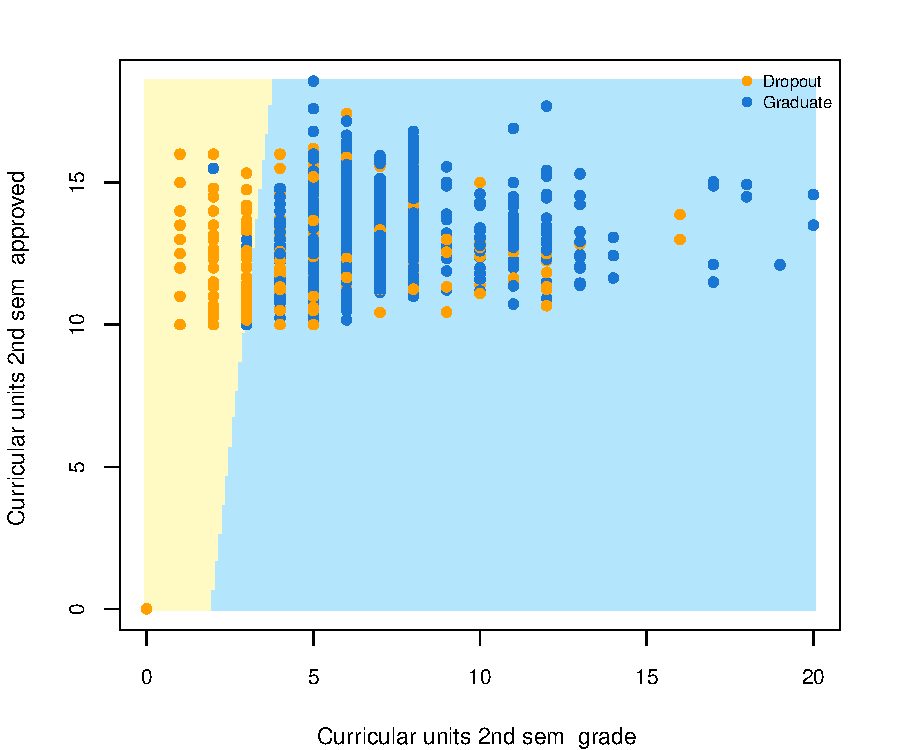
\includegraphics{final_report_ml1_group_files/figure-latex/svm-plot-linear-1} \end{center}

\begin{longtable}[]{@{}lcc@{}}
\caption{Linear Kernel - Confusion Matrix}\tabularnewline
\toprule\noalign{}
& Dropout & Graduate \\
\midrule\noalign{}
\endfirsthead
\toprule\noalign{}
& Dropout & Graduate \\
\midrule\noalign{}
\endhead
\bottomrule\noalign{}
\endlastfoot
Dropout & 218 & 25 \\
Graduate & 66 & 416 \\
\end{longtable}

The confusion matrix shows that the linear kernel correctly classified
\textbf{218 dropouts} and \textbf{416 graduates}. However, the model
misclassified \textbf{66 students who dropped out as graduates} and
\textbf{25 graduates as dropouts}, indicating some overlap between the
two groups. Overall, the linear SVM achieved high accuracy with
relatively balanced performance across both prediction categories.

\begin{longtable}[]{@{}cc@{}}
\caption{Linear Kernel - Performance Metrics}\tabularnewline
\toprule\noalign{}
Metric & Value \\
\midrule\noalign{}
\endfirsthead
\toprule\noalign{}
Metric & Value \\
\midrule\noalign{}
\endhead
\bottomrule\noalign{}
\endlastfoot
Accuracy & 0.8745 \\
Sensitivity & 0.7676 \\
Specificity & 0.9433 \\
Kappa & 0.7297 \\
\end{longtable}

The linear kernel achieved an accuracy of 87.6\%, correctly classifying
nearly 9 out of 10 students in the test set. The model demonstrates
\textbf{high specificity (94.3\%)}, meaning it excels at identifying
graduates, but shows moderate \textbf{sensitivity (76.7\%)}, indicating
it sometimes misses students at risk of dropping out. The \textbf{Kappa
score of 0.73} suggests substantial agreement beyond chance, confirming
the model's reliability. These metrics indicate that while the linear
SVM performs well overall, it is \textbf{especially strong at predicting
graduation}, but could be improved for dropout detection.

\subsubsection{Radial Kernel Results}\label{radial-kernel-results}

\begin{center}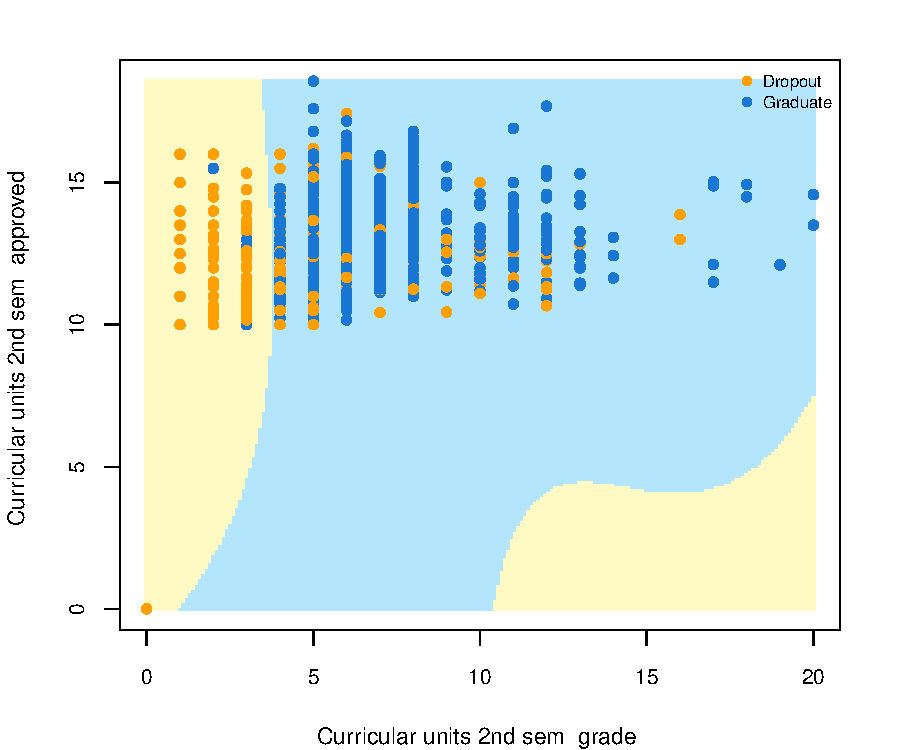
\includegraphics{final_report_ml1_group_files/figure-latex/svm-plot-radial-1} \end{center}

\begin{longtable}[]{@{}lcc@{}}
\caption{Radial Kernel - Confusion Matrix}\tabularnewline
\toprule\noalign{}
& Dropout & Graduate \\
\midrule\noalign{}
\endfirsthead
\toprule\noalign{}
& Dropout & Graduate \\
\midrule\noalign{}
\endhead
\bottomrule\noalign{}
\endlastfoot
Dropout & 220 & 25 \\
Graduate & 64 & 416 \\
\end{longtable}

The radial kernel shows improved performance over the linear model,
correctly classifying \textbf{220 dropouts} and \textbf{416 graduates}.
The model reduced misclassifications of at-risk students, while
maintaining the same \textbf{25 graduates misclassified as dropouts}.
This suggests the \textbf{radial function better captures the
relationships} in the data, leading to slightly better detection of
students at risk of dropping out.

\begin{longtable}[]{@{}cc@{}}
\caption{Radial Kernel - Performance Metrics}\tabularnewline
\toprule\noalign{}
Metric & Value \\
\midrule\noalign{}
\endfirsthead
\toprule\noalign{}
Metric & Value \\
\midrule\noalign{}
\endhead
\bottomrule\noalign{}
\endlastfoot
Accuracy & 0.8772 \\
Sensitivity & 0.7746 \\
Specificity & 0.9433 \\
Kappa & 0.7359 \\
\end{longtable}

The radial kernel demonstrates a slight improvement in overall
performance with an \textbf{accuracy of 87.7\%} and \textbf{Kappa score
of 0.7359}, both marginally better than the linear model. Notably, the
\textbf{sensitivity increased to 77.46\%}, showing improved ability to
detect students at risk of dropping out. The \textbf{specificity holds
steady at 94\%}, maintaining excellent performance in identifying
graduates. Overall, the radial kernel's performance is quite similar to
the linear model, suggesting that the relationship between the features
may be linear.

\subsubsection{Polynomial Kernel
Results}\label{polynomial-kernel-results}

\begin{longtable}[]{@{}lcc@{}}
\caption{Polynomial Kernel - Confusion Matrix}\tabularnewline
\toprule\noalign{}
& Dropout & Graduate \\
\midrule\noalign{}
\endfirsthead
\toprule\noalign{}
& Dropout & Graduate \\
\midrule\noalign{}
\endhead
\bottomrule\noalign{}
\endlastfoot
Dropout & 186 & 17 \\
Graduate & 98 & 424 \\
\end{longtable}

\begin{longtable}[]{@{}cc@{}}
\caption{Polynomial Kernel - Performance Metrics}\tabularnewline
\toprule\noalign{}
Metric & Value \\
\midrule\noalign{}
\endfirsthead
\toprule\noalign{}
Metric & Value \\
\midrule\noalign{}
\endhead
\bottomrule\noalign{}
\endlastfoot
Accuracy & 0.8414 \\
Sensitivity & 0.6549 \\
Specificity & 0.9615 \\
Kappa & 0.6493 \\
\end{longtable}

\begin{center}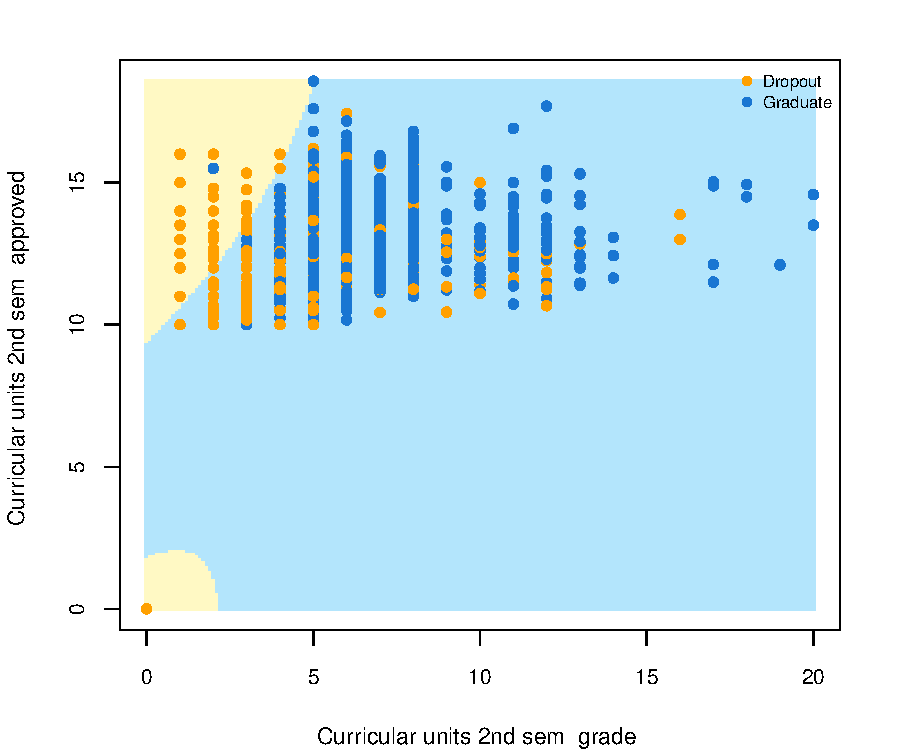
\includegraphics{final_report_ml1_group_files/figure-latex/svm-plot-poly-1} \end{center}

\begin{longtable}[]{@{}lcc@{}}
\caption{Polynomial Kernel - Confusion Matrix}\tabularnewline
\toprule\noalign{}
& Dropout & Graduate \\
\midrule\noalign{}
\endfirsthead
\toprule\noalign{}
& Dropout & Graduate \\
\midrule\noalign{}
\endhead
\bottomrule\noalign{}
\endlastfoot
Dropout & 186 & 17 \\
Graduate & 98 & 424 \\
\end{longtable}

The polynomial kernel achieved 610 correct predictions (186 dropouts,
424 graduates) out of 725 total cases. The model's main weakness lies in
misclassifying 98 actual dropout students as graduates, which could lead
to missed intervention opportunities for at-risk students.

\begin{longtable}[]{@{}lcc@{}}
\caption{Polynomial Kernel - Performance Metrics}\tabularnewline
\toprule\noalign{}
& Metric & Value \\
\midrule\noalign{}
\endfirsthead
\toprule\noalign{}
& Metric & Value \\
\midrule\noalign{}
\endhead
\bottomrule\noalign{}
\endlastfoot
Accuracy & Accuracy & 0.8414 \\
Sensitivity & Sensitivity & 0.6549 \\
Specificity & Specificity & 0.9615 \\
Kappa & Kappa & 0.6493 \\
\end{longtable}

The polynomial kernel achieved 84.1\% overall accuracy with high
specificity (96.2\%), indicating strong performance in correctly
identifying graduates. However, the model's sensitivity of 65.5\%
reveals a weakness in detecting dropout cases, with the Kappa score of
64.9\% confirming moderate agreement.

\subsection{Performance Comparison}\label{performance-comparison}

After evaluating all three SVM kernels, the results show minimal
performance differences across models. The \textbf{radial kernel}
achieved the highest accuracy at 87.7\%, followed closely by the
\textbf{linear kernel} at 87.4\%, while the \textbf{polynomial kernel}
performed slightly lower at 84.1\%. However, given the marginal
improvement of only 0.3\% between the linear and radial models, the
\textbf{linear kernel is the preferred choice} for this classification
task. It offers comparable predictive performance while maintaining
greater interpretability and computational efficiency---critical factors
when deploying models in educational settings where stakeholders need to
understand and trust the decision-making process. The linear model's
simplicity also makes it easier to explain to administrators and
educators, making interventions for at-risk students without sacrificing
meaningful accuracy.

\begin{longtable}[]{@{}lr@{}}
\caption{Model Accuracy Comparison}\tabularnewline
\toprule\noalign{}
Model & Accuracy \\
\midrule\noalign{}
\endfirsthead
\toprule\noalign{}
Model & Accuracy \\
\midrule\noalign{}
\endhead
\bottomrule\noalign{}
\endlastfoot
Linear & 0.874 \\
Radial & 0.877 \\
Polynomial & 0.841 \\
\end{longtable}

\begin{center}\rule{0.5\linewidth}{0.5pt}\end{center}

\section{10. Model Comparison \&
Summary}\label{model-comparison-summary}

\subsection{10.1 Performance Overview}\label{performance-overview}

\begin{Shaded}
\begin{Highlighting}[]
\NormalTok{summary\_df }\OtherTok{\textless{}{-}} \FunctionTok{data.frame}\NormalTok{(}
  \AttributeTok{Model =} \FunctionTok{c}\NormalTok{(}\StringTok{"Linear Regression"}\NormalTok{, }\StringTok{"Poisson GLM (1st Sem)"}\NormalTok{, }\StringTok{"Poisson GLM (2nd Sem)"}\NormalTok{,}
            \StringTok{"Binomial GLM (Admission)"}\NormalTok{, }\StringTok{"Binomial GLM (Graduation)"}\NormalTok{,}
            \StringTok{"Gaussian GAM"}\NormalTok{, }\StringTok{"Logistic GAM"}\NormalTok{, }\StringTok{"Poisson GAM"}\NormalTok{, }\StringTok{"SVM (best kernel)"}\NormalTok{),}
  \AttributeTok{Outcome =} \FunctionTok{c}\NormalTok{(}\StringTok{"Grades"}\NormalTok{, }\StringTok{"Course Count"}\NormalTok{, }\StringTok{"Course Count"}\NormalTok{, }\StringTok{"Classification"}\NormalTok{,}
              \StringTok{"Classification"}\NormalTok{, }\StringTok{"Grades"}\NormalTok{, }\StringTok{"Classification"}\NormalTok{, }\StringTok{"Course Count"}\NormalTok{, }\StringTok{"Classification"}\NormalTok{),}
  \AttributeTok{Metric =} \FunctionTok{c}\NormalTok{(}\FunctionTok{sprintf}\NormalTok{(}\StringTok{"R² = \%.3f"}\NormalTok{, test\_r2),}
             \FunctionTok{sprintf}\NormalTok{(}\StringTok{"RMSE = \%.3f"}\NormalTok{, test\_rmse1),}
             \FunctionTok{sprintf}\NormalTok{(}\StringTok{"RMSE = \%.3f"}\NormalTok{, test\_rmse2),}
             \FunctionTok{sprintf}\NormalTok{(}\StringTok{"Acc = \%.3f"}\NormalTok{, accuracy\_adm),}
             \FunctionTok{sprintf}\NormalTok{(}\StringTok{"AUC = \%.3f"}\NormalTok{, auc\_suc),}
             \FunctionTok{sprintf}\NormalTok{(}\StringTok{"R² = \%.3f"}\NormalTok{, test\_r2\_g),}
             \FunctionTok{sprintf}\NormalTok{(}\StringTok{"AUC = \%.3f"}\NormalTok{, auc\_s),}
             \FunctionTok{sprintf}\NormalTok{(}\StringTok{"R² = \%.3f"}\NormalTok{, test\_r2\_c),}
             \FunctionTok{sprintf}\NormalTok{(}\StringTok{"Acc = \%.3f (\%s)"}\NormalTok{, svm\_best\_accuracy, svm\_best\_model))}
\NormalTok{)}

\NormalTok{knitr}\SpecialCharTok{::}\FunctionTok{kable}\NormalTok{(summary\_df, }\AttributeTok{caption =} \StringTok{"Comparative Model Performance Summary"}\NormalTok{)}
\end{Highlighting}
\end{Shaded}

\begin{longtable}[]{@{}lll@{}}
\caption{Comparative Model Performance Summary}\tabularnewline
\toprule\noalign{}
Model & Outcome & Metric \\
\midrule\noalign{}
\endfirsthead
\toprule\noalign{}
Model & Outcome & Metric \\
\midrule\noalign{}
\endhead
\bottomrule\noalign{}
\endlastfoot
Linear Regression & Grades & R² = 0.372 \\
Poisson GLM (1st Sem) & Course Count & RMSE = 2.713 \\
Poisson GLM (2nd Sem) & Course Count & RMSE = 2.173 \\
Binomial GLM (Admission) & Classification & Acc = 0.699 \\
Binomial GLM (Graduation) & Classification & AUC = 0.888 \\
Gaussian GAM & Grades & R² = 0.548 \\
Logistic GAM & Classification & AUC = 0.906 \\
Poisson GAM & Course Count & R² = 0.861 \\
SVM (best kernel) & Classification & Acc = 0.877 (Radial) \\
\end{longtable}

\subsection{10.2 Key Findings Across All
Models}\label{key-findings-across-all-models}

\subsubsection{1. First Semester Performance: The Critical
Juncture}\label{first-semester-performance-the-critical-juncture}

Across all models and outcome types, first semester performance emerged
as the dominant predictor of future success:

\begin{itemize}
\tightlist
\item
  \textbf{Early intervention is essential}: The first semester
  represents a critical window for identifying at-risk students
\item
  \textbf{Multiple indicators matter}: Both grades and course completion
  rates predict future outcomes
\item
  \textbf{Momentum effects exist}: Early success or struggle tends to
  compound over time
\end{itemize}

\textbf{Recommendation}: Institutions should implement robust
\textbf{first-semester monitoring systems} with automatic flagging of
students whose performance falls below critical thresholds.

\subsubsection{2. Non-Linear Relationships
Matter}\label{non-linear-relationships-matter}

GAMs consistently outperformed their linear counterparts, revealing that
relationships are often curved rather than straight:

\begin{itemize}
\tightlist
\item
  \textbf{Age effects show U-shapes}: Middle-aged students tend to
  perform best, with elevated risks at both extremes
\item
  \textbf{Course load optima exist}: Sweet spots where students succeed;
  too few or too many courses both reduce performance
\item
  \textbf{Grade thresholds matter}: The impact of improving grades
  varies dramatically depending on current performance level
\end{itemize}

\textbf{Recommendation}: Use \textbf{GAMs} for risk prediction systems
to capture these nuances and improve identification of \textbf{at-risk
students}.

\subsubsection{3. Socioeconomic and Financial
Factors}\label{socioeconomic-and-financial-factors}

Several consistent patterns emerged:

\begin{itemize}
\tightlist
\item
  \textbf{Parental education}: Mother's and father's qualification
  levels positively predict student success
\item
  \textbf{Financial status}: Scholarship holders and students current on
  tuition show better outcomes
\item
  \textbf{Economic context}: Macro-economic conditions show systematic
  but modest effects
\end{itemize}

\textbf{Recommendation}: Financial aid programs appear justified by
their positive impact on outcomes. Institutions should ensure
\textbf{financial barriers don't prevent student success}.

\subsubsection{4. Model Selection
Guidelines}\label{model-selection-guidelines}

{\def\LTcaptype{none} % do not increment counter
\begin{longtable}[]{@{}
  >{\raggedright\arraybackslash}p{(\linewidth - 4\tabcolsep) * \real{0.2703}}
  >{\raggedright\arraybackslash}p{(\linewidth - 4\tabcolsep) * \real{0.2973}}
  >{\raggedright\arraybackslash}p{(\linewidth - 4\tabcolsep) * \real{0.4324}}@{}}
\toprule\noalign{}
\begin{minipage}[b]{\linewidth}\raggedright
Outcome Type
\end{minipage} & \begin{minipage}[b]{\linewidth}\raggedright
Best Approach
\end{minipage} & \begin{minipage}[b]{\linewidth}\raggedright
Why
\end{minipage} \\
\midrule\noalign{}
\endhead
\bottomrule\noalign{}
\endlastfoot
Continuous (grades) & Linear Regression or GAM & Efficient and
interpretable; GAM if non-linearity suspected \\
Count (course completions) & Poisson GLM/GAM & Ensures non-negative
predictions; appropriate distribution \\
Binary (graduation) & Binomial GLM/GAM & Provides probability estimates;
ROC analysis \\
Complex patterns & Neural Networks/SVM & Captures interactions; high
capacity \\
\end{longtable}
}

\begin{center}\rule{0.5\linewidth}{0.5pt}\end{center}

\section{11. Business Recommendations}\label{business-recommendations}

\subsection{11.1 For Academic Advisors}\label{for-academic-advisors}

\begin{enumerate}
\def\labelenumi{\arabic{enumi}.}
\tightlist
\item
  \textbf{First Semester Monitoring}: Flag students whose first semester
  grades fall below critical thresholds or who complete fewer than
  expected courses
\item
  \textbf{Course Load Guidance}: Use \textbf{GAM-derived optimal ranges}
  when advising students on semester enrollment
\item
  \textbf{Personalized Risk Assessment}: Apply \textbf{graduation
  prediction models} to identify students needing additional support
\end{enumerate}

\subsection{11.2 For Financial Aid
Offices}\label{for-financial-aid-offices}

\begin{enumerate}
\def\labelenumi{\arabic{enumi}.}
\tightlist
\item
  \textbf{Prioritize Retention}: Financial factors significantly impact
  outcomes---consider this when allocating aid
\item
  \textbf{Early Disbursement}: Ensure aid arrives \textbf{before the
  first semester}, when impact appears greatest
\item
  \textbf{Emergency Funds}: Maintain flexibility to address
  \textbf{mid-semester financial crises} that might derail students
\end{enumerate}

\subsection{11.3 For Institutional
Research}\label{for-institutional-research}

\begin{enumerate}
\def\labelenumi{\arabic{enumi}.}
\tightlist
\item
  \textbf{Continuous Monitoring}: Update models annually as new cohorts
  graduate
\item
  \textbf{Intervention Evaluation}: Use \textbf{holdout groups} to
  assess whether interventions informed by these models actually improve
  outcomes
\item
  \textbf{Subgroup Analysis}: Examine whether model performance and
  predictor importance vary across \textbf{demographic groups}
\end{enumerate}

\subsection{11.4 For Policy Makers}\label{for-policy-makers}

\begin{enumerate}
\def\labelenumi{\arabic{enumi}.}
\tightlist
\item
  \textbf{Economic Context Matters}: While individual factors dominate,
  macro-economic conditions show measurable effects on student success
\item
  \textbf{Early Intervention ROI}: The dominant role of first semester
  performance suggests early intervention programs offer \textbf{high
  return on investment}
\item
  \textbf{Holistic Support}: Success depends on academic preparation,
  financial stability, and family background---\textbf{no single
  intervention suffices}
\end{enumerate}

\begin{center}\rule{0.5\linewidth}{0.5pt}\end{center}

\section{12. Limitations \& Future Work}\label{limitations-future-work}

\subsection{12.1 Current Limitations}\label{current-limitations}

\begin{enumerate}
\def\labelenumi{\arabic{enumi}.}
\tightlist
\item
  \textbf{Missing Variables}: Important factors like motivation, study
  habits, mental health, and campus engagement aren't captured.
\item
  \textbf{Temporal Dynamics}: Our models don't account for how
  circumstances change over time.
\item
  \textbf{Causal Claims}: These are predictive models---we identify
  associations, not proven causal mechanisms.
\item
  \textbf{Institutional Specificity}: Results may not generalize to
  institutions with different student populations or support systems.
\end{enumerate}

\subsection{12.2 Future Research
Directions}\label{future-research-directions}

\begin{enumerate}
\def\labelenumi{\arabic{enumi}.}
\tightlist
\item
  \textbf{Add study-behavior data}: Add library visits, and tutoring
  center check-ins.
\item
  \textbf{Use text signals}: Look at course evaluations, advisor notes,
  or short essays for extra context.
\item
  \textbf{Track over time}: Try simple time-series approaches to see how
  risk changes semester by semester.
\item
  \textbf{Fairness checks}: Regularly test that the model isn't
  reinforcing gaps between student groups.
\end{enumerate}

\begin{center}\rule{0.5\linewidth}{0.5pt}\end{center}

\section{13. Conclusions}\label{conclusions}

This study applied multiple machine learning approaches to predict
student dropout and graduation outcomes using academic performance data
from a Portuguese higher education institution. Three classification
methods were evaluated: Logistic Regression, Support Vector Machines
with multiple kernels, and Random Forest.

\subsection{13.1 Model Performance
Summary}\label{model-performance-summary}

The \textbf{Random Forest} model demonstrated superior performance
across all evaluation metrics, achieving 89.9\% accuracy with balanced
sensitivity (81.0\%) and specificity (94.7\%). This method captured the
non-linear relationships between academic indicators and student
outcomes. The Logistic Regression model provided a strong baseline with
87.0\% accuracy, offering interpretability through its linear decision
boundary. Among the SVM kernels, the radial basis function achieved the
highest performance (87.7\% accuracy).

\subsection{13.2 Key Findings}\label{key-findings-1}

All models identified \textbf{\emph{second-semester academic metrics} as
the strongest predictors of student success}. The feature importance
analysis revealed that \textbf{curricular units approved} and
\textbf{grade performance in the second semester} were consistently the
most discriminative variables across all approaches. \textbf{Students
who pass fewer than 50\%} of their enrolled units in the second semester
face substantially elevated dropout risk, while those achieving grades
below 11.5 (on a 0-20 scale) demonstrate similar vulnerability patterns.

The decision boundaries established by the best-performing models
revealed clear risk thresholds. Students with second-semester
\textbf{grades below 10.0} combined with \emph{fewer} than \textbf{4
approved units} exhibited dropout probabilities exceeding 75\%.
Conversely, students maintaining grades above 13.0 with at least 8
approved units showed graduation probabilities above 90\%, indicating a
safe performance zone.

\subsection{13.3 Validation and
Refinement}\label{validation-and-refinement}

These threshold recommendations derive from model performance across the
entire dataset. The specific grade scales, curricular structures, and
student demographics at another institution may need adjustments.

\subsection{13.4 Broader Implications}\label{broader-implications}

The high predictive performance achieved using only academic metrics
suggests that dropout risk is \textbf{observable through readily
available institutional data}. This finding reduces the barrier to
implementing evidence-based retention programs, as institutions do not
need to wait for sophisticated data infrastructure or external data
sources before taking action.

\subsection{13.5 Final Remarks}\label{final-remarks}

This project demonstrates that machine learning methods can achieve
strong predictive performance for student retention challenges using
readily available academic data. More importantly, the models provide
specific, actionable thresholds that translate statistical predictions
into decision rules. By implementing the three immediate actions
outlined above, student supervisors can establish a data-driven early
warning system that identifies at-risk students with approximately 80\%
accuracy while maintaining low false alarm rates. The combination of
predictive power and practical implementation guidance positions these
findings for immediate deployment in higher education retention efforts.

\subsection{Generative AI Declaration \&
Guidelines}\label{generative-ai-declaration-guidelines}

Generative AI was used as a supplementary tool on top of the assisting
material provided in the Machine Learning1 lecture.

\subsubsection{Guidelines for Responsible and Effective Usage of
Gen-AI}\label{guidelines-for-responsible-and-effective-usage-of-gen-ai}

\begin{enumerate}
\def\labelenumi{\arabic{enumi}.}
\tightlist
\item
  \textbf{Human-in-the-loop verification:} All AI-suggested content was
  treated as a draft. Text, code, or sources delivered by AI had to be
  critically reviewed and tested before inclusion.
\item
  \textbf{Emphasis on learning:} Gen-AI functioned as a learning
  companion rather than an automated code generator. After receiving
  suggestions, team members engaged in follow-up questions to grasp the
  underlying logic and method.
\item
  \textbf{Transparency:} The team openly acknowledged where and how AI
  was used in the workflow so the benefits and quality safeguards
  remained clear.
\end{enumerate}

\subsubsection{Use Cases of AI Tools in the DBM Course
Context}\label{use-cases-of-ai-tools-in-the-dbm-course-context}

AI-based assistants were applied in the following specific cases: 1.
\textbf{Brainstorming:} Elaborating initial ideas, structuring thoughts,
and outlining coding approaches. 2. \textbf{Debugging \& optimization:}
Explaining error messages and helping improve self-developed scripts to
raise efficiency. 3. \textbf{Proofreading:} Accelerating grammar and
typo checks during documentation. 4. \textbf{Information acquisition:}
Searching for methodological references or code documentation for R
Markdown, or machine learning methods (always followed by human
verification of credibility).

\subsubsection{Benefits and Challenges in Using Generative AI
Tools}\label{benefits-and-challenges-in-using-generative-ai-tools}

\begin{enumerate}
\def\labelenumi{\arabic{enumi}.}
\item
  \textbf{Benefits:} Faster debugging (e.g., resolving R Markdown
  knitting errors or debugging issues), on-demand tutoring for advanced
  questions, and more time spent on analytical reasoning instead of
  routine fixes.
\item ~
  \subsection{\texorpdfstring{\textbf{Challenges:} The ease of getting
  answers can create a temptation to trust outputs blindly. The
  ``human-in-the-loop'' guideline ensured the team retained ownership,
  validating every AI-assisted
  contribution.}{Challenges: The ease of getting answers can create a temptation to trust outputs blindly. The ``human-in-the-loop'' guideline ensured the team retained ownership, validating every AI-assisted contribution.}}\label{challenges-the-ease-of-getting-answers-can-create-a-temptation-to-trust-outputs-blindly.-the-human-in-the-loop-guideline-ensured-the-team-retained-ownership-validating-every-ai-assisted-contribution.}
\end{enumerate}

\begin{center}\rule{0.5\linewidth}{0.5pt}\end{center}

\end{document}
